\documentclass[11pt,twoside,a4paper]{book}
%
% Unitex manual
%
\usepackage[english]{babel}
\selectlanguage{english}
\usepackage{palatino}
\usepackage[T1]{fontenc}
\usepackage{epsfig}
\usepackage{makeidx,color}
\usepackage{graphicx}
\title{Unitex 2.0 User Manual}
\author{S�bastien Paumier - Universit� Paris-Est Marne-la-Vall�e}
\date{2008}


\usepackage[%
%%              ps2pdf,
%%              dvips,
             pdfauthor={S�bastien Paumier},
             pdftitle={Unitex User Manual},
             pdfcreator={LaTeX, hyperref},
             pdfkeywords={corpus linguistics, computational linguistics,
             finite state automata / transducer, local grammar, lexicon grammar}, pdfsubject={Manual of Unitex, a corpus processing system, based on automata-oriented technology},
             %final, % use hyperlinks ever
             bookmarks,
             backref,
%%              breaklinks=true,
             colorlinks=true,
             urlcolor=blue,
%%              linkcolor=black,
%%              citecolor=black,
%%              anchorcolor=black,
             pdfpagemode=None,
           % pdfpagemode=FullScreen,
             pdfstartview=FitBH,
             unicode,
             ]{hyperref}



%
% d�finitions de commandes
%
%\newcommand{\httplink}[1]{\textcolor{blue}{\underline{\texttt{http://#1}}}}
\newcommand{\E}{$\varepsilon$}
\newcommand{\exemplemauvais}[1]{\textit{* #1}}
\newcommand{\exemplebon}[1]{\textit{#1}}
\newcommand{\exemplebizarre}[1]{\textit{? #1}}
\newcommand{\exempletresbizarre}[1]{\textit{*? #1}}
\pagenumbering{arabic}
\global\setlength{\topmargin}{-1.5cm}
\global\setlength{\footskip}{2cm}
\global\setlength{\headheight}{1.5cm}
\global\setlength{\headsep}{0.3cm}
\global\setlength{\textheight}{21.5cm}
\global\setlength{\oddsidemargin}{0.5cm}
\global\setlength{\evensidemargin}{0.5cm}
\global\setlength{\marginparwidth}{1.5cm}
\global\setlength{\textwidth}{15.5cm}
\makeindex

\begin{document}


\begin{titlepage}
\begin{center}

~

\vspace{3cm}
\Huge
\textsc{\textbf{Unitex 2.1}}

\vspace{1cm}

\huge
\textsc{\textbf{User Manual}}

\vspace{2cm}

  \begin{center}
    \includegraphics[width=4cm]{resources/img/logo-Unitex.png}
  \end{center}
\normalsize

\vspace{2cm}

\LARGE

Universit� Paris-Est Marne-la-Vall�e
\bigskip
\normalsize

\url{http://www-igm.univ-mlv.fr/~unitex}

\verb$unitex@univ-mlv.fr$

\vspace{1cm}

%\today
S�bastien Paumier
\bigskip

English translation of previous version by the local grammar group at the\\
 CIS, Ludwig-Maximilians-Universit�t, Munich - Oct 2003\\
 (Wolfgang Flury, Franz Guenthner, Friederike Malchok, Clemens Marschner, Sebastian Nagel, Johannes Stiehler)

\url{http://www.cis.uni-muenchen.de/}
\end{center}

\end{titlepage}


\tableofcontents

\chapter*{Introduction}
\addcontentsline{toc}{chapter}{Introduction}

Unitex is a collection of programs developped for the analysis of texts in
natural language by using linguistic resources and tools. These resources
consist of electronic dictionaries, grammars and lexicon-grammar tables,
initially developed  for French by Maurice Gross and his students  at the
Laboratoire d'Automatique Documentaire et Linguistique (LADL).\index{LADL}
Similar resources have been developed for other languages in the context of the
RELEX laboratory network.

\bigskip
\noindent The electronic dictionaries specify the simple and compound words of a
language together with their lemmas and a set of grammatical (semantic and inflectional)
codes. The availability of these dictionaries is a major advantage compared to
the usual utilities for pattern searching as the information they contain can be
used  for searching and matching,  thus  describing large classes of words using
very simple patterns. The dictionaries are presented in the DELA formalism and
were constructed  by teams of  linguists for several languages (French, English,
Greek, Italian, Spanish, German, Thai, Korean, Polish, Norwegian, Portuguese,
etc.)

\bigskip
\noindent The grammars used here are representations of linguistic phenomena on the
basis of  recursive transition networks (RTN), a formalism closely related to
finite state automata. Numerous studies have shown the adequacy of automata for
linguistic problems at all descriptive levels  from morphology and syntax to
phonetic issues. Grammars created with Unitex carry this approach further  by
using a formalism even more powerful than automata. These grammars are
represented as graphs that the user can easily create and update.

\bigskip
\noindent Lexicon-grammar tables are matrices describing
properties of some words. Many such tables have been constructed   for all
simple verbs in French as a way of describing their relevant
syntactic properties. Experience has shown that every word has a
quasi-unique behavior, and these tables are a way to present the 
grammar of every element in the lexicon, hence the name lexicon-grammar 
for this linguistic theory. Unitex offers a way to
automatically build grammars from lexicon-grammar tables.

\bigskip
\noindent Unitex can be viewed as a tool in which one can put linguistic resources
and use them. Its technical characteristics are its portability,  modularity,
the possibility of dealing with languages that use special writing systems (e.g. many
Asian languages), and its openness, thanks to its open source distribution. Its
linguistic characteristics are the ones that have motivated the elaboration of
these resources: precision, completeness, and the taking into account of frozen
expressions, most notably those which concern the enumeration of compound words.


\section*{What's new from version 1.2 ?}
\addcontentsline{toc}{section}{What's new from version 1.2 ?}
Here are some interesting new features:
\begin{itemize}
  \item left contexts
  \item morphological mode in \verb$Locate$
  \item brand new version of \verb$Convert$
  \item replacement of \verb$Inflect$ by \verb$MultiFlex$ that can inflect compound words
  and that can handle consonant skeletons for semitic languages
  \item introduction of the text alignment tool \verb$XAlign$
  \item no size limit for text file display
  \item SVG export of graphs
\end{itemize}

\bigskip \noindent From a computational point of view, a special effort has been
made to clean and comment the source code of Unitex programs in order to
facilitate the integration of new components. Moreover, the development of Unitex
is now made with a SVN server, which makes collaborative work much more easier.


\section*{Content}
\addcontentsline{toc}{section}{Content}
\noindent Chapter \ref{chap-installation} describes how to install and run
Unitex.

\bigskip \noindent Chapter \ref{chap-texte} presents the different steps in the
analysis of  a text.

\bigskip \noindent Chapter \ref{chap-dictionaries} describes the formalism of
the DELA electronic dictionaries and the different operations that can be applied to them.

\bigskip \noindent Chapters \ref{chap-regexp} and \ref{chap-grammaires-locales}
present different means for making text searches more effective. 
Chapter \ref{chap-grammaires-locales} describes in detail how to use the graph
editor.

\bigskip \noindent Chapter \ref{chap-grammaires-avanc�es} is concerned with the
different possible applications of grammars. The particularities of each type of grammar are
presented.

\bigskip \noindent Chapter \ref{chap-automate-du-texte} introduces the  concept
of text automaton and describes the properties of this notion. This chapter also describes 
operations on this object, in particular, how to disambiguate lexical items with
the ELAG program.

\bigskip \noindent Chapter \ref{chap-lexique-grammaire} contains an introduction
to lexicon-grammar tables, followed by a description of the method of constructing grammars based on these
tables.

\bigskip \noindent Chapter \ref{chap-alignment} describes the text
alignment module, based on the XAlign tool.

\bigskip \noindent Chapter \ref{chap-multiflex} describes the compound word
inflection module, as a complement of the simple word inflection mechanism
presented in chapter \ref{chap-dictionaries}.

\bigskip \noindent Chapter \ref{chap-programmes-externes} contains a detailed
description of the external programs that make up the Unitex system.

\bigskip \noindent Chapter \ref{chap-formats-de-fichiers} contains descriptions
of all file formats used in the system.


\bigskip \noindent The reader will find in appendix the GPL and LGPL licenses
under which the Unitex source code is released, as well as the LGPLLR license
which applies for the linguistic data distributed with Unitex.

\chapter{Installation of Unitex}
\label{chap-install}

Unitex is a multi-platform system that runs on Windows as well as on Linux or
MacOS. This chapter describes how to install and how to launch Unitex on any of
these systems. It also presents the procedures used to add new languages and to
uninstall Unitex.

\section{Licenses}
\label{section-licences}
\index{LGPL}\index{License!LGPL}
Unitex is a free software. This means that the sources of the programs are
distributed with the software, and that anyone can modify and redistribute them.
The code of the Unitex programs is under the LGPL licence (\cite{LGPL}), except
for the TRE library for dealing with regular expressions from Ville Laurikari
(\cite{TRE}), which is under 2-clause BSD licence which is more
permissive than the LGPL. The LGPL Licence is more permissive than the GPL
licence, because it makes it possible to use LGPL code in nonfree software. 
From the point of view of the user, there is no difference,
because in both cases, the software can freely be used and distributed.

\bigskip
\noindent All the data that go with Unitex are distributed under the LGPLLR
license \index{LGPLLR} (\cite{LGPLLR}).

\bigskip
\noindent Full text versions of LGPL, 2-clause BSD and LGPLLR can be found in
the appendices of this manual.

\section{Java runtime environment}
Unitex consists of a graphical interface written in Java and external programs
written in \textit{C/C\kern-.05em\raisebox{.5ex}{++}\kern-.1em}. This mixture of
programming languages is responsible for a fast and portable application that
runs on different operating systems.

\bigskip
\noindent Before you can use the graphical interface, you first have to install the runtime
environment, usually called Java virtual machine \index{Java virtual machine} or
JRE\index{JRE} (Java Runtime Environment\index{Java Runtime Environment}).

\bigskip
\noindent For the graphical mode, Unitex needs Java version 1.6 (or newer). If you have an
older version of Java, Unitex will stop after you have chosen the working
language.

\bigskip
\noindent You can download the virtual machine for your operating system for free from the
Sun Microsystems web site (\cite{site-java}) at the following address:
\url{http://java.sun.com}.

\bigskip
\noindent If you are working under Linux or MacOS, or if you are using a Windows version
with personal user accounts, you have to ask your system administrator to install
Java.


\section{Installation on Windows}
\index{Installation!on Windows}
If Unitex is to be installed on a multi-user Windows machine, it is recommended
that the systems administrator performs the installation. If you are the only
user on your machine, you can perform the installation  yourself.

\bigskip
\noindent Decompress the file \index{File!\verb+unitex_2.0.zip+} \verb+unitex_2.0.zip+ (You
can download this file from the following address:
\url{http://www-igm.univ-mlv.fr/~unitex}) into a directory \verb+Unitex+ that
should preferably be created within the \verb+Program Files+ folder.

\bigskip
\noindent After decompressing the file, the \verb+Unitex+ directory contains several
subdirectories  one  of which is called \verb+App+. This directory contains a
file called \verb+Unitex.jar+. \index{File!\verb+Unitex.jar+} This file is the
Java executable that launches the graphical interface. You can double click on
this icon to start the program. To facilitate launching Unitex, you may want to
add a shortcut to this file on the desktop.




\section{Installation on Linux}
\index{Installation!on Linux}
In order to install Unitex on Linux, it is recommended to have system
administrator permissions. Uncompress the file \verb+Unitex2.1.zip+ in a
directory named \verb+Unitex+, by using the following command:

\bigskip \noindent \verb$unzip Unitex2.1.zip -d Unitex$

\bigskip
\noindent Within the directory \verb|Unitex/Src/C++/build|, start the compilation
of Unitex with the command:

\bigskip \verb+make install+

\bigskip
\noindent or with the following if you have a 64 bits computer:
 
\bigskip \verb+make install 64BITS=yes+

\bigskip
\noindent You can then create an alias in the following way:

\bigskip \verb$alias unitex='cd /..../Unitex/App/ ; java -jar Unitex.jar'$


\section{Installation on MacOS X}
\index{Installation!on MacOS X}
\label{section-macos-install}
\noindent NOTE: this short tutorial will tell you how to install and run 
Unitex on Mac OS X. Your questions, comments, suggestions, 
corrections are more than welcome. 

\noindent Contact: \url{cedrick.fairon@uclouvain.be}

\bigskip
\noindent There is an official Java 1.6 for MacOS X 10.5, 64-bit Intel 
(Core 2 Duo), but there is no official solution for older OS X (10.4 or older),
PowerPC and 32-bit Intel (Core Duo). So,
\begin{enumerate}
    \item if you have OS X 10.5, and 64-bit Intel MacOS, you can just get the
    Apple JRE 1.6. The only problem is that this version does not start by
    default. See section ``Java for Mac OS X 10.5 Update 2'', 
    at \url{http://developer.apple.com/java/}

    \item if you have an older OS X, 32-bit Intel or a PowerPC, you must try
    SoyLatte (see below)
\end{enumerate}

\noindent\textbf{How to know if my processor is a 32 or 64-bit one ?}

\noindent In the Apple menu, click on "About this Mac". If you see something
like: "Processor : x.xx Ghz Intel Core Duo", your processor is a 32-bit one.

\bigskip
\noindent If you see "Processor : x.xx Ghz Intel Core 2 Duo", or if you
processor is another Intel one (like Xeon), then you have a 64-bit processor.

\subsection{Using the Apple Java 1.6 runtime}
\bigskip\index{Using the Apple Java 1.6}
\noindent If you are running Mac OS X 10.5 (or later) on 64-Bits Intel processor, you can just use the Java 1.6 from Apple.\ You can get it from \url{http://www.apple.com/support/downloads/javaformacosx105update1.html}.

\noindent\ You can just start Application -> Utilities -> Java Preferences to verify the status of Java 1.6. First, be sure that "Java SE 6" is on "Java Applications" list
\begin{figure}[!h]
\begin{center}
\includegraphics[width=13cm]{resources/img/java_pref_osx.png}
\caption{Checking and modify Java Preferences\label{fig-mac0}}
\end{center}
\end{figure}


\subsubsection{Option 1 : modify the default runtime for Java Applications}
\noindent If you don't use other Java application that need Java 1.5, you can just put "Java SE 6" at the top of the "Java Applications" list on Java Preference Utility.

\subsubsection{Option 2 : Create an alias to start Java 1.6}
\noindent If you don't want modify Java global parameters, you can create an
alias:

\bigskip
\noindent \verb+alias jre6="/System/Library/Frameworks/JavaVM.framework/Versions/+
\noindent \verb+1.6/Commands/java"+
   
\bigskip
\noindent \verb+jre6 -jar Unitex.jar+

\bigskip
\noindent Then just run Unitex from Terminal.

\subsection{SoyLatte}
\bigskip\index{SoyLatte}
\noindent SoyLatte is a functional, X11-based port of the FreeBSD
Java 1.6 patchset to Mac OS X Intel machines. SoyLatte is initially focused on 
supporting Java 6 development; however, the long-term view far more captivating: 
open development of Java 7 for Mac OS X, with a release available in concert 
with the official Sun release, supported on all recent versions of Mac OS X.

\subsubsection{Before you start}
\noindent Try it at your own risks ;-) This tutorial tells you what I have done
to have Unitex running on my MacBook Pro (Mac OS X 10.5.7), but it offers no guarantee 
that it will work  on your computer and it does not even guarantee that you can 
install it safely on your computer.

\bigskip
\noindent If you are not familiar with software installation, you should ask for
help. As Windows would put it ``Contact your Administrator'' ;-) 

\bigskip
\noindent It works only on Intel based Macintosh If you do not know whether your 
Macintosh is an Intel machine or not, select in the Apple Menu the item 
``About this Macintosh'', then, click on ``More info'' and in the next panel,
click on ``Hardware'', as shown on Figure \ref{fig-mac1}.

\begin{figure}[!h]
\begin{center}
\includegraphics[width=13cm]{resources/img/fig-mac1.png}
\caption{Getting information on your computer\label{fig-mac1}}
\end{center}
\end{figure}

\clearpage

\subsubsection{Installation}
\noindent Some of the following installation steps will require the use of the
terminal application. On MacOS, the terminal application is located in 
\verb+/Applications/Utilities/Terminal.app+.  When you start this application
(double click) a window is displayed. You will have to type in this window 
some commands for moving, editing and installing files.

\subsubsection{Install X11.app}
\index{X11.app}
\noindent X11 is available as an optional install on the Mac OS X v10.3 
Panther, and Mac OS X v10.4 Tiger install disks (the disks you received 
when you bought your computer). Run the Installer, 
select the X11 option, and follow the instructions.

\bigskip
\noindent After installation X11 will be available in
\verb+/Applications/Utilities/+


\subsubsection{Download and install Unitex as usual}
\noindent Download Unitex and uncompress it in the same way that for Linux.
See section \ref{section-mac-compilation} for instructions on compiling
C++ programs.


\subsubsection{Download SoyLatte (the Java 1.6 port)} 
\noindent It is available from
\url{http://landonf.bikemonkey.org/static/soylatte/} 

\bigskip
\noindent Unless you know why you need another package, you will chose 
the 32-Bit Binaries distribution (32-bit JDK for Mac OS X 10.4 and 10.5) 
When prompted, enter the username and password: 

\bigskip
Username: \verb+jrl+

Password: \verb+I am a Licensee in good standing+


\subsubsection{Install SoyLatte}
\noindent Either in command line mode:
\begin{itemize}
    \item Open the terminal (\verb+/Applications/Utilities/Terminal+)
    \item Find the SoyLatte archive. If it is on your desktop, change the
    current directory by typing the following command in the terminal 
    (the character \verb+~+ means 'home directory'): 
    
    \bigskip
    \verb+cd ~/Desktop/+
    
    \item Move (\verb+mv+) the archive anywhere on your file system (where you
    want to install it). If you chose \verb+/usr/local+, like me, it requires the
    administrative privileges (use \verb+sudo+ and type your password when
    prompted). Note, if the directory does not exist, you can create it 
    before you move the file:
    
    \bigskip
    \verb+sudo mkdir /usr/local         + (only if it does not exist)
    
    \verb+sudo mv soylatte16-i386-1.0.3.tar.bz2 /usr/local/+

    \item Uncompress the archive:
    
    \bigskip
    \verb+sudo tar -jxvf /usr/local/soylatte16-i386-1.0.3.tar.bz2+ 
\end{itemize}

\bigskip
\noindent or, using the graphical interface (finder):
\begin{itemize}
    \item Move (drag and drop) the archive
    
    %do not remove this line jump
    \noindent \verb+soylatte16-i386-1.0.3.tar.bz2+ into the \verb+/Applications+ folder
    \item Double-click on it... wait... it's done ;-)
\end{itemize}


\subsubsection{Configure your system}
\noindent There are two approaches: you could either decide to use SoyLatte only
with Unitex (and keep using the former version of Java that is already installed 
on your computer for all the others Java applications) or decide to make SoyLatte 
the default Java distribution on your machine.

\bigskip
\noindent As I have no indication that SoyLatte is bug free and fully
functional with all applications, I chose to use SoyLatte only with 
Unitex and kept my Java (and I recommend the same for you). If you 
want to follow this advice: DO NOT modify your PATH variable as suggested 
in the SoyLatte installation procedure. Instead add an ALIAS in the configuration 
file of your shell. Here is how to do that:
\begin{itemize}
    \item Edit the bash configuration file, which is in your home directory 
    (\verb+/Users/your_dir_name+); The easiest way to do it is to use a command
    line editor like \verb+vim+ or \verb+pico+ (note: \verb+.bashrc+ is a hidden
    file. So, normally, you will not see this file in the Finder):
    
    \bigskip
    \verb+pico ~/.bashrc+
    
    \item In the file, type the following lines :
    
    \bigskip
    \verb+alias java6='/usr/local/soylatte16-i386-1.0.3/bin/java'+
    
    \verb+alias unitex='cd /Applications/Unitex21beta/App ; java6 -jar+
    
    \verb+Unitex.jar'+
    
    \bigskip
    \noindent The first line creates and alias that makes it easy to run
    SoyLatte-Java and the second line creates and alias that makes it easy to start Unitex.
    
    \item Then, quit \verb+pico+ (type CTRL+x, answer ``yes'' to the question
    ``Do you want to save?'' and then press Enter to proceed).
\end{itemize}

\noindent Changes will be active next time the \verb+.bashrc+ file is loaded
(quit and re-launch \verb+Terminal.app+ or more simply, type \verb+bash+ to open
a new bash session). Once you have a new bash session, type the command 
\verb+unitex+ and let's start using Unitex on your Mac !!

\begin{figure}[!h]
\begin{center}
\includegraphics[width=13cm]{resources/img/fig-mac2.png}
\caption{Running Unitex on Mac\label{fig-mac2}}
\end{center}
\end{figure}

\subsection{How to compile Unitex C++ programs on a Macintosh}
\label{section-mac-compilation}
\noindent In order to install Unitex on Mac OS, you will have to compile
Unitex C++ sources. This is not a problem if you have already the common 
(\verb+gcc+) development tools installed on your computer (but of course, they
are not in the standard installation).

\bigskip
\noindent If you don't know if these tools are present, don't think too long
about it... just give a try; open a shell window, move to the Unitex sources
directory (\verb$cd /path/to/Src/C++/build$) and run the command that starts the
compilation: \verb+make install+

\begin{figure}[!h]
\begin{center}
\includegraphics[width=12cm]{resources/img/fig-mac3.png}
\caption{Compiling Unitex C++ programs\label{fig-mac3}}
\end{center}
\end{figure}

\bigskip
\noindent If the compilation does not start and you get an error message
stating that the command \verb+make+ cannot be found, you probably need to
install development programs. On Macintosh the ``all inclusive development
bundel'' is ``Xcode'' \index{Xcode}(current version is 2.2 and it includes a lot
of stuff among which). Your can donwload it from the Appel developer Web site.

\bigskip
\noindent The Xcode application includes a full-featured code editor, a debugger, 
compilers, and a linker. The Xcode application provides a user interface to many 
industry-standard and open-source tools, including \verb+gcc+, the Java compilers
\verb+javac+ and \verb+jikes+, and \verb+gdb+. It provides all of the facilities you
need to build a program for Mac OS X, whether it's an application, kernel
extension, or command-line tool.

\bigskip
\noindent The only problem with Xcode is that it is HUGE to download (800 Mb).
Of course, you will not need all the stuff included in the package... but all
what you need is in it.

\begin{figure}[!h]
\begin{center}
\includegraphics[width=15cm]{resources/img/fig-mac4.png}
\caption{Xcode\label{fig-mac4}}
\end{center}
\end{figure}


\bigskip
\noindent Once on your computer the Xcode package looks like the following:

\begin{figure}[!h]
\begin{center}
\includegraphics[width=14cm]{resources/img/fig-mac5.png}
\caption{Xcode package\label{fig-mac5}}
\end{center}
\end{figure}


\bigskip
\noindent Double-click on the \verb+XCodeTools.mpkg+ icon to install all the
programs.


\subsection{How to makes all files visible on Mac OS}
\noindent See
\url{http://www.macworld.com/article/51830/2006/07/showallfinder.html}.

\bigskip
\noindent Or try it right away... Type: 

\bigskip
\verb+defaults write com.apple.Finder AppleShowAllFiles ON+

\bigskip
\noindent Then restart the Finder:

\bigskip
\verb+killall Finder+

\begin{figure}[!h]
\begin{center}
\includegraphics[width=12cm]{resources/img/fig-mac6.png}
\caption{Restarting the Finder\label{fig-mac6}}
\end{center}
\end{figure}

\bigskip
\noindent To get back to the original configuration, type: 

\bigskip
\verb+defaults write com.apple.Finder AppleShowAllFiles OFF+


\section{First use}
If you are working on Windows, the program will ask you to choose a
\index{Directory!personal working} personal working  directory, which you can
change later in "Info>Preferences...>Directories". To create a directory, click
on the icon showing a file (see
figure~\ref{fig-creation-personal-directory}).

\bigskip
\noindent If you are using Linux or MacOS, the program will automatically create a
\verb+/unitex+ directory in your \verb+$HOME+ directory. This directory allows
you to save your personal data. For each language that you will be using, the
program will copy the root directory of that language to your personal
directory, except the dictionaries. You can then modify your copy of the
files without risking to damage the system files.

\begin{figure}[h]
\begin{center}
\includegraphics[width=6.3cm]{resources/img/fig1-1.png}
\caption{First use under Windows}
\end{center}
\end{figure}

\begin{figure}[h]
\begin{center}
\includegraphics[width=7cm]{resources/img/fig1-2.png}
\caption{First use under Linux}
\end{center}
\end{figure}

\begin{figure}[h]
\begin{center}
\includegraphics[width=13cm]{resources/img/fig1-3.png}
\caption{Creating the personal work
directory\label{fig-creation-personal-directory}}
\end{center}
\end{figure}



\section{Adding new languages}
\index{Adding languages}

\bigskip
\noindent There are two different ways to add languages. If you want to add 
a language that is to be accessible by all  users, you have to copy the 
corresponding directory to the \verb+Unitex+ system directory, for which 
you will need to have the access rights  (this might mean that you need to 
ask your system administrator to do it). On the other hand, if the language 
is only used by a single user, he can also copy the directory to his working 
directory. He can work with this language without this language being shown to other users.


\section{Uninstalling Unitex}
No matter which operating system you are working with, it is sufficient to delete 
the \verb+Unitex+ directory to completely delete all the program files. Under
Windows you may have to delete the shortcut to \verb+Unitex.jar+ \index{File!\verb+Unitex.jar+} 
if you have created one on your desktop. The same has to be done on Linux, if you have 
created an alias.


\section{Unitex for developpers}
\label{section-unitex-developpers}
If you are a programmer, you may be interested in linking your code with Unitex
C++ sources. To facilitate such operation, you can compile Unitex as a
dynamic library that contains all Unitex functions, except \verb+main+s, of
course. Under Linux/MacOS, type:

\bigskip
\verb+make LIBRARY=yes+

\bigskip
\noindent and you will obtain a library named \verb+libunitex.so+. If you want
to produce a Windows DLL named \verb+unitex.dll+, use the following commands:

\bigskip
Windows: \verb+make SYSTEM=windows LIBRARY=yes+

Cross-compiling with mingw32: \verb+make SYSTEM=mingw32 LIBRARY=yes+

\bigskip
\noindent In all cases, you will also obtain a program named
\verb+Test_lib+(\verb+.exe+). If everything worked fine, this program should 
display the following:

\begin{verbatim}
Expression converted.
Reg2Grf exit code: 0

#Unigraph
SIZE 1313 950
FONT Times New Roman:  12
OFONT Times New Roman:B 12
BCOLOR 16777215
FCOLOR 0
ACOLOR 12632256
SCOLOR 16711680
CCOLOR 255
DBOXES y
DFRAME y
DDATE y
DFILE y
DDIR y
DRIG n
DRST n
FITS 100
PORIENT L
#
7
"<E>" 100 100 1 5
"" 100 100 0
"a" 100 100 1 6
"b" 100 100 1 4
"c" 100 100 1 6
"<E>" 100 100 2 2 3
"<E>" 100 100 1 1
\end{verbatim}

\chapter{Loading a text}
\label{chap-texte}

One of the main functionalities of Unitex is to search a text for expressions.
To do that, texts have to undergo a set of preprocessing steps that  normalize
non-ambiguous forms and split the text  in sentences. Once these operations are
performed, the electronic dictionaries are applied to the texts. Then one  can
search more effectively in the texts by using  grammars.

\bigskip
\noindent This chapter describes the different steps for text preprocessing.


\section{Selecting a language}
\index{Selecting a language}\index{Language selection}
When starting Unitex, the program asks you to choose the language in which you
want to work (see figure~\ref{fig-s�lection-langue}). The languages displayed are
the ones that are present in the \verb+Unitex+ system directory and those that
are  installed in your personal working directory. If you use a language for the
first time, Unitex copies the system directory for this language to your personal
directory, except for the dictionaries in order to save disk space.

\bigskip
\noindent WARNING: If
you already have a personal directory for a given language, Unitex won't try to
copy system data into it. So, if an update has modified a resource file other
than a dictionary, you will have to copy by yourself this file, or to delete your
personal directory for this language, and let Unitex rebuild it properly.

\bigskip
\noindent 
Choosing the language allows Unitex to find certain files, for example the
alphabet file. \index{File!alphabet} You can change the language at any time by
choosing "Change Language..." in the "Text" menu. If you change the language, the
program will close all windows related to the current text, if there are any. The
active language is indicated in the title bar of the graphical interface.

\begin{figure}[!h]
\begin{center}
\includegraphics[width=6.2cm]{resources/img/fig2-1.png}
\caption{\label{fig-s�lection-langue}Language selection when starting Unitex}
\end{center}
\end{figure}


\section{Text formats}
\label{section-conversion-texte-unicode}
\index{Text!formats}
\index{Corpus|see{Text}}
\index{Unicode}
Unitex works with Unicode texts. Unicode is a standard that describes a universal
character code. Each character is given a unique number, which allows for
representing texts without having to take into account  the proprietary codes on
different machines and/or operating systems. Unitex uses a two-byte
representation of the Unicode 3.0 standard, called Unicode Little-Endian (for
more details, see \cite{UNICODE}).

\bigskip
\index{File!transcoding}
\noindent Texts that come with Unitex are already in Unicode format. If you try
to open a text that is not in Unicode, the program proposes to convert it
(see figure~\ref{auto-transcoding}).
This conversion is based on the current language: if you are working in French,
Unitex proposes to convert your text\,\footnote{Unitex also proposes to
automatically convert graphs and dictionaries that are not in Unicode
Little-Endian.} assuming that it is coded using a French code page. By default,
Unitex proposes to either replace the original text or to rename the original
file by inserting \verb$.old$ at the beginning of  its extension. For example, if
one has an ASCII file named \verb$balzac.txt$, the conversion process will create
a copy of this ASCII file named \verb$balzac.old.txt$, and will replace the
contents of \verb$balzac.txt$ with its equivalent in Unicode.


\begin{figure}[!h]
\begin{center}
\includegraphics[width=10cm]{resources/img/fig2-2.png}
\caption{\label{auto-transcoding}Automatic conversion of a non-Unicode text}
\end{center}
\end{figure}

\noindent If the encoding suggested by default is not correct  or if you want to
rename the file differently than with the suffix \verb$.old$, you must use the "Transcode Files" command
in the "File Edition" menu. This command allows you to choose source and
target encodings of the documents to be converted (see figure~\ref{transcoding}). By default,
the selected source encoding is that which corresponds to the current language
and the destination encoding is Unicode Little-Endian. You can modify these choices by selecting
any source and target encodings. Thus, if you wish, you can convert your data
into other encodings, as for example UTF-8 in order for instance to create web pages. The button
"Add Files" enables you to select the files to be converted. The button "Remove Files" makes it
possible to remove a list of files erroneously selected. The button "Transcode" will start the
conversion of all the selected files. If an error occurs with a file is
processed (for example, a file which is already in Unicode), the 
conversion continues with the next file.


\begin{figure}[!h]
\begin{center}
\includegraphics[width=12cm]{resources/img/fig2-3.png}
\caption{\label{transcoding}Transcoding files}
\end{center}
\end{figure}

\noindent To obtain a text in the right format, you can also use a text
processor like the free software from OpenOffice.org  (\cite{OpenOffice}) or Microsoft Word, and
save your document with the format "Unicode text".
In OpenOffice Writer, you have to choose the "Coded Text (*.txt)" format and then
select the "Unicode" encoding in the configuration window as shown on figure
\ref{OfficeWriter}.

\begin{figure}[!h]
\begin{center}
\includegraphics[width=12.5cm]{resources/img/fig2-4.png}
\caption{\label{OfficeWriter}Saving in Unicode with OpenOffice Writer}
\end{center}
\end{figure}

\noindent By default, the encoding proposed on a PC is always Unicode
Little-Endian. The texts thus obtained do not contain any formatting information anymore (fonts,
colors , etc.) and are ready to be used with Unitex.


\section{Editing text files}
You also have the possibility of using the text editor integrated into Unitex,
accessible via the "Open..." command in the "File Edition" menu".
\index{Integrated text editor} This editor offers search and replace
functionalities  for the texts and dictionaries handled by Unitex. To use it,
click on the "Find" icon. You will then see a window  divided into three parts.
The "Find" part corresponds to the usual search operations. If you open a text
split into sentences, you can base your search on sentence numbers 
in the "Find Sentence" part. Lastly, the "Search Dictionary" part,
visible in figure~\ref{dictionary-search}, enables you to carry out operations
concerning the electronic dictionaries. In particular, you can   search by
specifying if it concerns  inflected forms, lemmas, grammatical and semantic
and/or inflectional codes. Thus, if you want to search for all the verbs which
have the  semantic feature \verb$t$\index{\verb$t$}, which indicates
transitivity, you just have to search for  \verb$t$ by clicking on "Grammatical
code". You will get the matching entries without confusion  with all the other
occurrences of the letter \verb$t$.


\begin{figure}[!h]
\begin{center}
\includegraphics[width=15cm]{resources/img/fig2-5.png}
\caption{Searching an electronic dictionary for the semantic feature \texttt{t}\label{dictionary-search}}
\end{center}
\end{figure}


\section{Opening a text}
Unitex deals with two types of text files. \index{File!text}
The files with the extension \verb+.snt+ are text files preprocessed by Unitex
which are ready to be manipulated by the different system functions. The files
ending with \verb+.txt+ are raw files.
To use a text, open the \verb+.txt+ file by clicking on "Open..." in the "Text"
menu. Choose the file type "Raw Unicode Texts" and select your text.

\begin{figure}[!h]
\begin{center}
\includegraphics[width=14cm]{resources/img/fig2-6.png}
\caption{Text Menu}
\end{center}
\end{figure}

\begin{figure}[!h]
\begin{center}
\includegraphics[width=13cm]{resources/img/fig2-7.png}
\caption{Opening a Unicode text}
\end{center}
\end{figure}

 

\section{Preprocessing a text}
\index{Text!preprocessing}
After a text is selected, Unitex offers to preprocess it. Text preprocessing
consists of performing the following operations: normalization of separators,
splitting into sentences, normalization of non-ambiguous forms, tokenization and 
application of dictionaries. If you choose not to preprocess the text, it 
will nevertheless be normalized and tokenized, since
these operations are necessary for all further Unitex operations. It is always
possible to carry out the preprocessing later by clicking on "Preprocess Text..."
in the "Text" menu. 

\begin{figure}[!h]
\begin{center}
\includegraphics[width=15cm]{resources/img/fig2-8.png}
\caption{Preprocessing Window\label{fig-fen�tre-de-pr�traitement}}
\end{center}
\end{figure}

\bigskip
\noindent 
If you choose to preprocess the text, Unitex proposes to parameterize it
as in the window shown in figure~\ref{fig-fen�tre-de-pr�traitement}.
The option "Apply FST2 in MERGE mode" is used to split the text into sentences.
The option "Apply FST2 in REPLACE mode" is used to make replacements in the text,
especially for the normalization of non-ambiguous forms. With the option "Apply
All default Dictionaries" you can apply dictionaries in the DELA format
(Dictionnaires Electroniques du LADL).\index{DELA} The option "Analyze unknown
words as free compound words" is used in Norwegian for correctly analyzing
compound words  constructed via concatenation of simple forms.  Finally, the
option "Construct Text Automaton" is used to build the text automaton. This
option is deactivated by default, because it consumes a large amount of memory
and disk space if the text is too large. The construction of the text automaton
is described in chapter~\ref{chap-automate-du-texte}.

\bigskip
\noindent NOTE: If you click on "Cancel but tokenize text", the program will
carry out the normalization of separators and split the text into tokens. Click
on "Cancel and close text" to cancel the operation.

\subsection{Normalization of separators}
\index{Normalization!of separators}\index{Separators}\index{Text!normalization}
The standard separators are the space, the tab and the newline characters. There
can be several separators following each other, but since this isn't useful for
linguistic analyses, separators are normalized according to the following rules:

\begin{itemize}
  \item a sequence of separators that contains at least one newline is replaced by a single newline
  
  \item all other sequences of separators are replaced by a single space.
\end{itemize}

\bigskip
\noindent 
The distinction between space and newline is maintained at this point because the
presence of newlines may have an effect on the process of splitting the text into
sentences. The result of the normalization of a text named  \verb+my_text.txt+ is
a file in the same directory as the \verb+.txt+ file and is named
\verb+my_text.snt+. \index{File!\verb+.snt+}

\bigskip
\noindent NOTE: When the text is preprocessed using the graphical interface, a
directory named

% do not remove this line jump 
\noindent \verb+my_text_snt+ is created immediately after normalization.
This directory, called text directory,  \index{Directory!text}
\index{Text!directory} contains all the data associated with this text.



\subsection{Splitting into sentences}
\label{section-d�coupage-en-phrases}
\index{Splitting into sentences}\index{Text!splitting into sentences}
\index{Grammars!splitting into sentences}
Splitting texts into sentences is an important preprocessing step since  this
helps in determining the units for linguistic processing. The splitting is used
by the text automaton construction program. In contrast to what one might think,
detecting sentence boundaries is not a trivial problem. Consider the following
text:

\bigskip
\textit{The family has urgently called Dr. Martin.}

\bigskip \noindent The full stop that follows \textit{Dr} is followed by a word
beginning with a capital letter. Thus it may be considered as the end of the
sentence, which would be wrong. To avoid the kind of problems caused by the
ambiguous use of punctuation, grammars are used to  describe the different
contexts for the end of a sentence.
Figure~\ref{fig-exemple-d�coupage-en-phrases} shows an example grammar for
sentence splitting (for French sentences).

\bigskip
\noindent When a path of the grammar recognizes a sequence in the text and when
this path produces the sentence delimiter symbol \verb+{S}+
\index{\verb+{S}+}\index{Sentence separator}, this symbol is inserted into the
text.

\bigskip
\noindent The path shown at the top of figure~\ref{fig-exemple-d�coupage-en-phrases}
recognizes the sequence consisting of a question mark and a word beginning with a
capital letter and inserts the symbol \verb+{S}+ between the question mark and
the following word. The following text:

\bigskip
\textit{What time is it? Eight o' clock.}

\bigskip
\noindent will be converted to:

\bigskip
\textit{What time is it ?\{S\} Eight o' clock.}

\bigskip
\noindent A  grammar for end-of-sentence detection may use the following
special symbols:

\index{\verb+<E>+}\index{Epsilon|see{<E>}}
\index{\verb+<MOT>+}\index{\verb+<MIN>+}\index{\verb+<MAJ>+}\index{\verb+<PRE>+}\index{\verb+<NB>+}
\index{\verb+<PNC>+}\index{\verb+<^>+}\index{\verb+#+}\index{Meta-symbols}
\begin{itemize}
  \item <E> : empty word, or epsilon. Recognizes the empty sequence;
  \item <MOT> : recognizes any sequence of letters;
  \item <MIN> : recognizes any sequence of letters in lower case;
  \item <MAJ> : recognizes any sequence of letters in upper case;
  \item <PRE> : recognizes any sequence of letters that begins with an upper case letter;
  \item <NB> : recognizes any sequence of digits (1234 is recognized but not 1
  234); \item <PNC> : recognizes the punctuation symbols \verb+ ; , ! ? :+ and the
  inverted exclamation points and question marks in Spanish and some Asian
  punctuation letters; \item <\verb+^+> : recognizes a newline; \item \verb+#+ :
  prohibits the presence of a space.
\end{itemize}

\begin{figure}[!h]
\begin{center}
\includegraphics[width=15cm]{resources/img/fig2-9.png}
\caption{Sentence splitting grammar for French\label{fig-exemple-d�coupage-en-phrases}}
\end{center}
\end{figure}

\bigskip
\noindent By default, the space is optional between two boxes. If you want to prohibit the
presence of the space you have to use the special character  \verb+#+. At the
opposite, if you want to force the presence of the space, you must use the
sequence \verb+" "+. Lower and upper case letters are defined by an alphabet
file\index{File!alphabet} (see chapter~\ref{chap-formats-de-fichiers}). For more
details on grammars, see chapter~\ref{chap-grammaires-locales}.\index{Alphabet}
For more information about sentence boundary detection, see
\cite{ameliorer-decoupage-en-phrases}. The grammar used here is named
\verb+Sentence.fst2+ and can be found in the following directory:
\index{File!\verb+Sentence.fst2+}

\bigskip
\verb+/(user home directory)/(language)/Graphs/Preprocessing/Sentence+

\bigskip
\noindent This grammar is applied to a text with the \verb+Fst2Txt+ program
\index{\verb+Fst2Txt+}\index{External programs!\verb+Fst2Txt+} in
MERGE mode.\index{MERGE} This has the effect that the output produced
by the grammar, in this case the symbol \verb+{S}+, is inserted into
the text. This program takes a \verb+.snt+ file and modifies it.


\subsection{Normalization of non-ambiguous forms}
\index{Normalization!of non-ambiguous forms}
\index{Grammars!normalization!of non-ambiguous forms}

Certain forms present in texts can be normalized (for example, the English
sequence "\textit{I'm}" is equivalent to "\textit{I am}"). You may want to
replace these forms according to your own needs. However, you have to be careful
that the  forms normalized  are unambiguous or that the removal of ambiguity has
no undesirable consequences.

\bigskip
\noindent For instance, if you want to normalize "\textit{O'clock}" to "\textit{on the
clock}", it would be a bad idea to replace "\textit{O'}" by "\textit{on the }",
because a sentence like:

\bigskip
\textit{John O'Connor said: "it's 8 O'clock"}

\bigskip
\noindent would be replaced by the following incorrect sentence:

\bigskip
\textit{John on the Connor said: "it's 8 on the clock"}

\bigskip
\noindent Thus, one needs to be very careful when using the
normalization grammar. One needs to pay attention to spaces as well. 
For example, if one replaces "'re" by "are", the sentence:

\bigskip
\textit{You're stronger than him.}

\bigskip
\noindent will be replaced by:

\bigskip
\textit{Youare stronger than him.}

\bigskip
\noindent To avoid this problem, one should explicitly insert a space,
\textit{i.e.} replace "\textit{'re}" by "\textit{ are}".

\bigskip
\noindent The accepted symbols for the normalization grammar are the same as the ones
allowed for the sentence splitting grammar. The normalization grammar is called
\verb+Replace.fst2+ and can be found in the following directory:

\bigskip \verb+/(home directory)/(active language)/Graphs/Preprocessing/Replace+

\bigskip
\noindent As in the case of sentence splitting, this grammar is applied using the
\verb+Fst2Txt+ \index{External programs!\verb+Fst2Txt+}\index{\verb+Fst2Txt+}
program, but in REPLACE mode, which means that input sequences recognized by the
grammar are replaced by the output sequences that are produced.
Figure~\ref{fig-grammaire-de-normalisation} shows a grammar that normalizes
verbal contractions in English.

\begin{figure}[!p]
\begin{center}
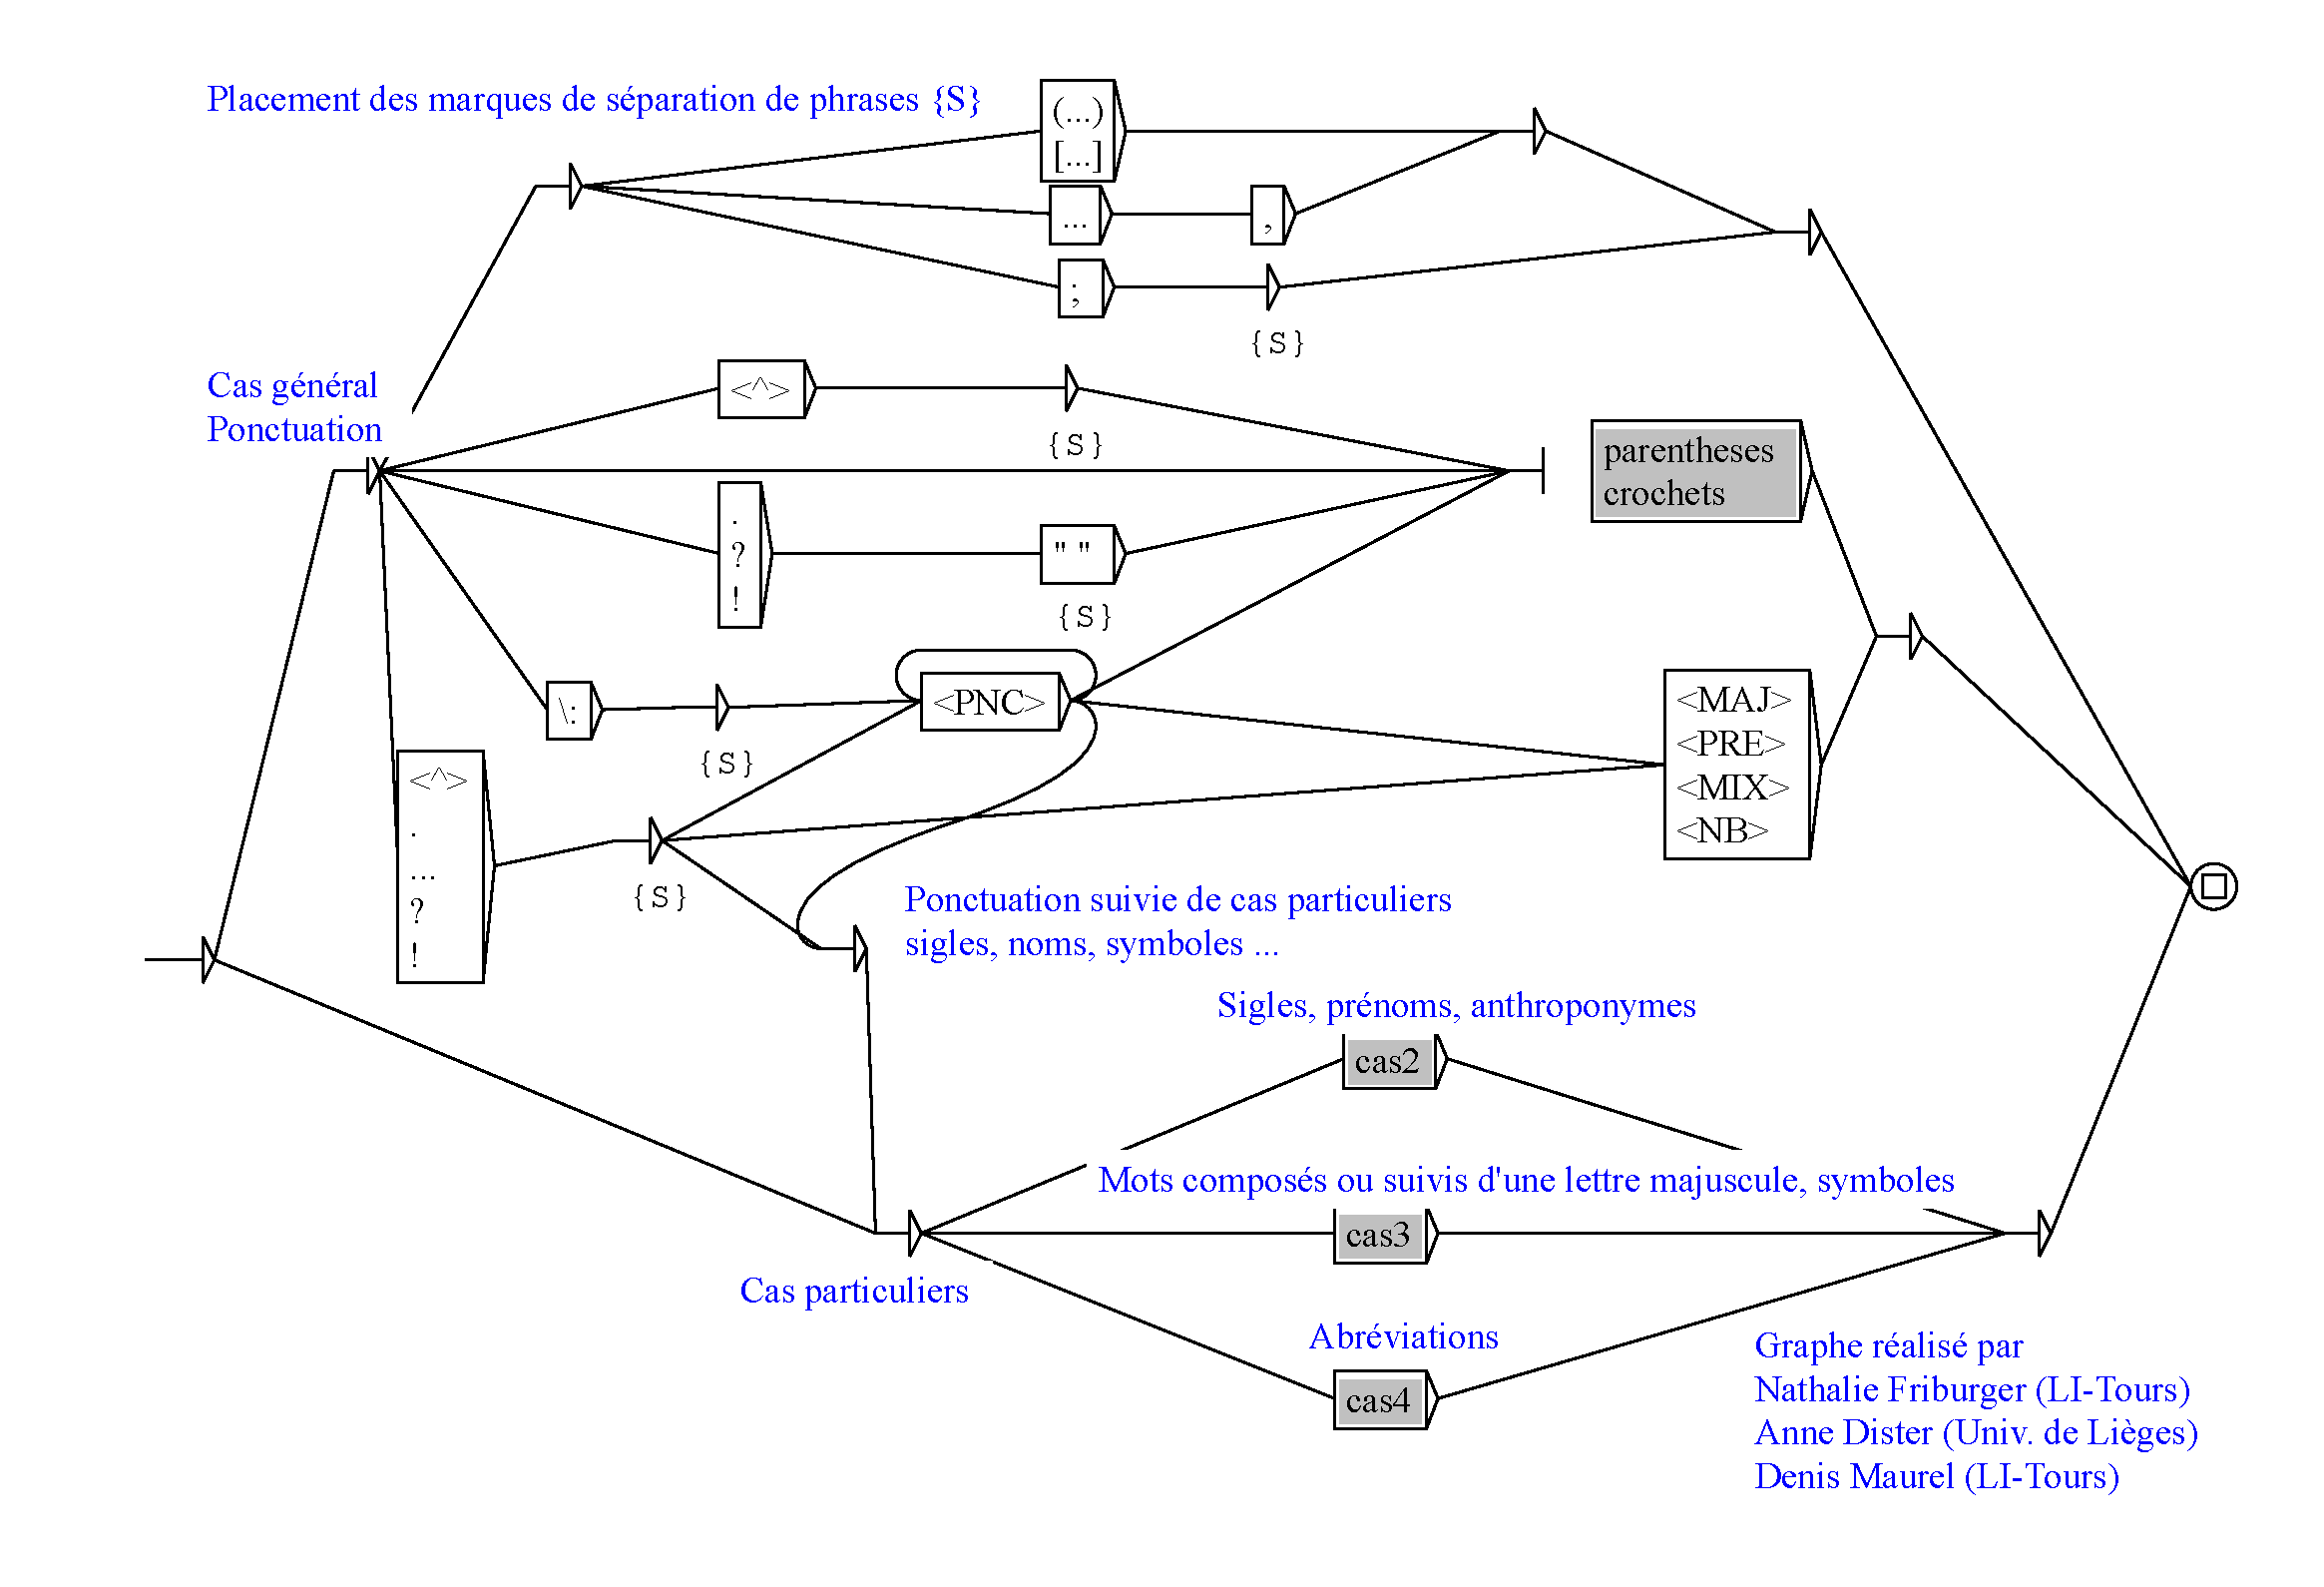
\includegraphics[width=14cm]{resources/img/fig2-10.png}
\caption{Normalization of English verbal contractions\label{fig-grammaire-de-normalisation}}
\end{center}
\end{figure}



\subsection{Splitting a text into tokens}
\index{Text!tokenization}
\index{Text!splitting into tokens}
\index{Token}
\index{Tokenization}
\label{decoupage-du-texte}
Some languages, in particular Asian languages, use separators that are different
from the ones used in  western languages. Spaces can be forbidden, optional, or
mandatory. In order to better cope with these particularities,  Unitex splits
texts in a language dependent way. Thus, languages like English are treated as
follows:

\bigskip
\noindent A token can be:
\begin{itemize}
  \item the sentence delimiter \verb+{S}+; \item the stop marker
  \verb+{STOP}+.\index{\verb${STOP}$} This token is a special one that can
  NEVER be matched in any way by a grammar. It can be used to bound elements
  in a corpus. For instance, if a corpus is made of news separated by
  \verb+{STOP}+, it will be impossible that a grammar matches a sequence that
  overlaps the end of a news and the beginning of the following news;
  \item a lexical tag \verb+{aujourd'hui,.ADV}+; \item a contiguous sequence of
  letters (the letters are defined in the language alphabet file);
  \index{File!alphabet}
  \item one (and only one) non-letter character, i.e. all characters not defined
  in the alphabet file of the current language; if it is a newline, it is replaced by
  a space.
\end{itemize}

\bigskip
\noindent For other languages, tokenization is done on a character by character
basis, except for the sentence delimiter \verb+{S}+, the \verb+{STOP}+ marker
and lexical tags. This simple tokenization is fundamental for the use of Unitex,
but limits the optimization of search operations for patterns.

\bigskip
\noindent Regardless of the tokenization mode, newlines in a text are
replaced by spaces. Tokenization is done by the \verb+Tokenize+\index{\verb+Tokenize+}
\index{External programs!\verb+Tokenize+} program. This program creates several
files that are saved in the text directory:
\begin{itemize}
  \item \verb+tokens.txt+ contains the list of tokens in the order in which they are found in the text;
  \index{File!\verb+tokens.txt+}
  \item \verb+text.cod+ contains an integer array; every
  integer corresponds to the index of a token in the file \verb+tokens.txt+;
  \index{File!\verb+text.cod+}
  \item \verb+tok_by_freq.txt+ contains the list of tokens sorted by frequency;
  \index{File!\verb+tok_by_freq.txt+}
  \item \verb+tok_by_alph.txt+ contains the list of tokens in alphabetical order;
  \index{File!\verb+tok_by_alph.txt+}
  \item \verb+stats.n+ contains some statistics about the text. \index{File!\verb+stats.n+}
\end{itemize}

\bigskip
\noindent Tokenizing the text:

\bigskip
\textit{A cat is a cat.}

\bigskip
\noindent returns the following list of tokens: \textit{A} SPACE \textit{cat is a .}

\bigskip
\noindent You will observe that tokenization is case sensitive (\textit{A} and
\textit{a} are two distinct tokens), and that each token is listed only once.
Numbering these tokens from 0 to 5, the text can be represented by a sequence of
numbers (integers) as described in the following table:

\bigskip
\begin{table}[h]
\begin{center}
\begin{tabular}{|p{2.8cm}||c|c|c|c|c|c|c|c|c|c|c|c|}
\hline
Token number               & 0 & 1 & 2 & 1 & 3 & 1 & 4 & 1 & 2 & 5
\\
\hline
Corresponding token & \textit{A} &   & \textit{cat} &   & \textit{is} &  & \textit{a}
& & \textit{cat} & \textit{.}
\\
\hline
\end{tabular}
\caption{Representation of the text \textit{A cat is a cat.}}
\end{center}
\end{table}

\bigskip
\noindent For more details, see chapter~\ref{chap-formats-de-fichiers}.

\begin{figure}[!h]
\begin{center}
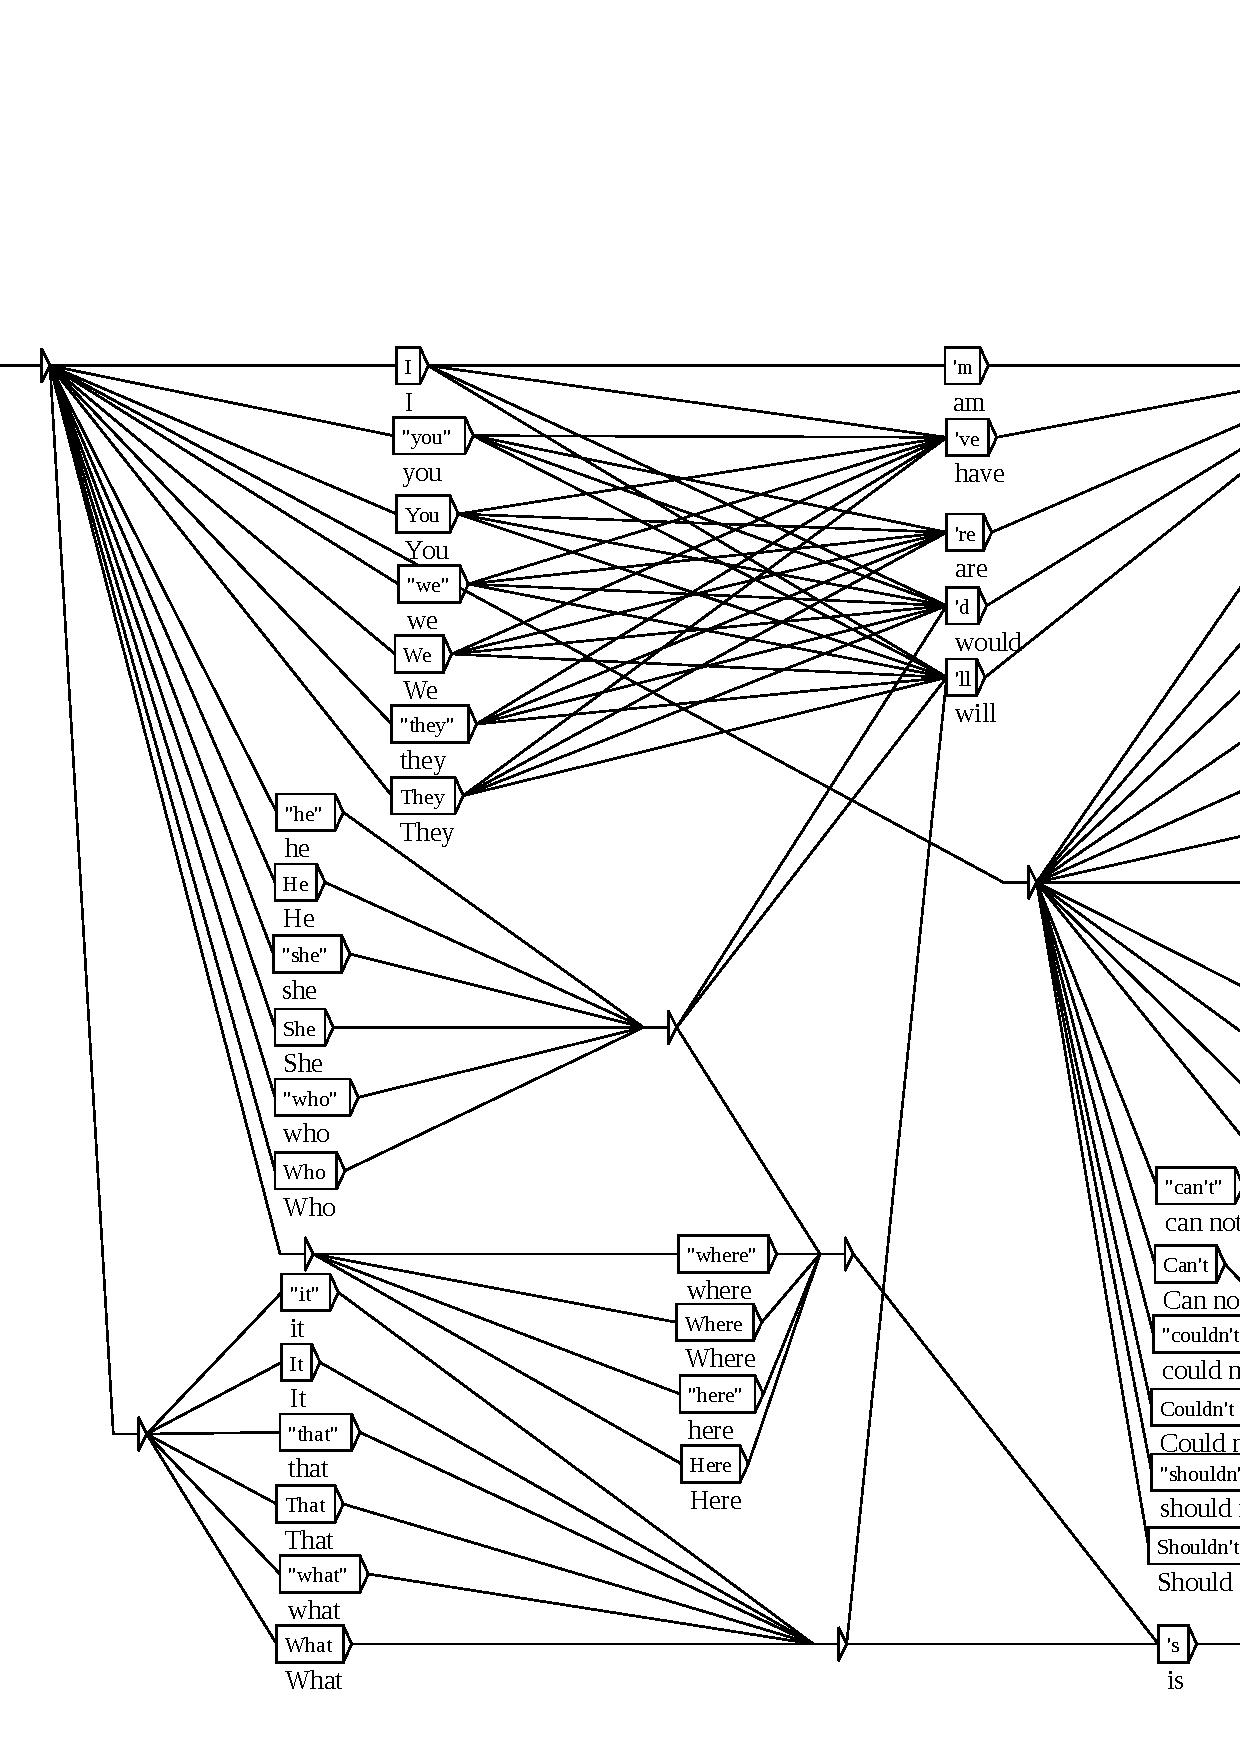
\includegraphics[height=10cm]{resources/img/fig2-11.png}
\caption{Tokens of an English text sorted by frequency}
\end{center}
\end{figure}



\subsection{Applying dictionaries}
\index{Dictionaries!applying}
\index{Lexical!resources|see {Dictionaries}}
Applying dictionaries consists of building the subset of dictionaries  consisting
only of forms that are present in the text. Thus, the result of applying a
English dictionary to the text \textit{Igor's father in law is ill} produces a
dictionary of the following simple words:\index{Words!simple}

\bigskip
\begin{verbatim}
father,.N+Hum:s
father,.V:W:P1s:P2s:P1p:P2p:P3p
ill,.A
ill,.ADV
ill,.N:s
in,.A
in,.N:s
in,.PART
in,.PREP
is,be.V:P3s
is,i.N:p
law,.N:s
law,.V:W:P1s:P2s:P1p:P2p:P3p
s,.N:s
\end{verbatim}

\bigskip
\noindent as well as a dictionary of compound words consisting of a single
entry:\index{Words!compound}

\bigskip
\begin{verbatim}
father in law,.N+NPN+Hum+z1:s
\end{verbatim}

\bigskip
\noindent Since the sequence \textit{Igor} is neither a simple English word nor a part of a
compound word, it is treated as an unknown word. \index{Words!unknown} The
application of dictionaries is done through the program \verb+Dico+.
\index{\verb+Dico+}\index{External programs!\verb+Dico+} The three files produced
(\verb+dlf+ for simple words, \verb+dlc+ for compound words and \verb+err+ for
unknown words) are placed in the text directory. The \verb+dlf+ and \verb+dlc+
files are called text dictionaries.  \index{Dictionaries!text}
\index{File!\verb+dlf+}
\index{File!\verb+dlc+}\index{File!\verb+err+}

\bigskip
\noindent As soon as the dictionary look-up  is finished, Unitex displays the sorted lists
of simple, compound and unknown words found in a new window.
Figure~\ref{fig-r�sultat-application-dictionnaires} shows the result for an
English text.

\begin{figure}[!ht]
\begin{center}
\includegraphics[width=12cm]{resources/img/fig2-12.png}
\caption{Result after applying dictionaries to an English text\label{fig-r�sultat-application-dictionnaires}}
\end{center}
\end{figure}

\bigskip
\noindent It is also possible to apply dictionaries without preprocessing the text. In
order to do this, click on "Apply Lexical Resources..." in the "Text" menu.
Unitex then opens a window (see
figure~\ref{fig-param�trage-application-dictionnaires}) in which you can select
the list of dictionaries to apply.

\begin{figure}[!ht]
\begin{center}
\includegraphics[width=10cm]{resources/img/fig2-13.png}
\caption{Parameterizing the application of dictionaries\label{fig-param�trage-application-dictionnaires}}
\end{center}
\end{figure}

\bigskip
\noindent The list "User resources" lists all dictionaries present in the
directory

% DO NOT REMOVE THIS LINE JUMP!
\noindent \verb+(current language)/Dela+ of the user. The dictionaries installed
in the system are listed in the scroll list  named "System resources". Use the
<Ctrl+click> combination to select several dictionaries. System dictionaries
will be applied prior to user dictionaries. Within the system or user list, you
can fix the order of dictionaries using the up and down arrows, as shown on
figure \ref{fig-param�trage-application-dictionnaires}. The button "Set
Default" allows you to define the current selection of dictionaries  as the
default. This default selection will then be used during preprocessing if you
activate the option "Apply All default Dictionaries".\index{Dictionaries!default
selection} If you right-click on a dictionary name, the associated documentation,
if any, will be displayed in the lower frame of the window.


\subsection{Analysis of compound words in Dutch, German, Norwegian and Russian}
\index{Norwegian!compound words}\index{Analysis of compound words in Norwegian}
\index{Words!compound!in Norwegian}
\index{German!compound words}\index{Analysis of compound words in German}
\index{Words!compound!in German}
\index{Russian!compound words}\index{Analysis of compound words in Russian}
\index{Words!compound!in Russian}
\index{Words!compound!in Dutch}
\label{section-mots-compos�s-libres-en-norv�gien}
In certain languages like Norwegian, German and others, it is possible to form
new compound words by concatenating  together other words. For example, the word
\textit{aftenblad} meaning \textit{evening journal} is obtained by combining the
words \textit{aften} (\textit{evening}) et \textit{blad} (\textit{journal}). The
\verb+PolyLex+ program \index{\verb+PolyLex+}\index{External
programs!\verb+PolyLex+} parses the list of unknown words after the application
of dictionaries and tries to analyze each of these words as a compound word. If
a word has at least one analysis as a compound word,  it is removed from the
list of unknown words and the lines produced for this word are appended to the
simple word text dictionary.



\section{Opening a tagged text}
A tagged text is a text containing words with lexical tags enclosed in round brackets:

\bigskip
\textit{I do not like the \{square bracket,.N\} sign! \{S\}}

\bigskip
\noindent Such tags can be used to avoid ambiguities. In the previous example,
it will be impossible to match \textit{square bracket} as the combination of two
simple words.

\bigskip
\noindent However, the presence of these tags can alter the application of
preprocessing graphs. To avoid complications, you can use the "Open Tagged
Text..." command in the "Text" menu. With it, you can open a tagged text and skip
the application of preprocessing graphs, as shown on Figure
\ref{preprocess-tagged-text}.

\bigskip
\begin{figure}[!h]
\begin{center}
\includegraphics[width=14cm]{resources/img/fig2-14.png}
\caption{Preprocessing a tagged text\label{preprocess-tagged-text}}
\end{center}
\end{figure}

\input{03-dictionaries}
\chapter{Searching with regular expressions}
\label{chap-regexp}

This chapter describes how to search a text for simple patterns by using regular
expressions.

\section{Definition}
\index{Regular expressions}

The goal of this chapter is not to give an introduction on formal languages but
to show how to use regular expressions in Unitex in order to search for simple
patterns. Readers who are interested in a more formal presentation can consult
the many works that discuss regular expression patterns.

\bigskip \noindent A regular expression can be:

\begin{itemize}
  \item a token (\verb+book+) or a lexical mask
  (\verb+<smoke.V>+);
  \item the concatenation of two regular
  expressions (\verb+he smokes+);\index{Concatenation of regular expressions}
  \item the union of two regular expressions (\verb$Pierre+Paul$);\index{Union of
  regular expressions} 
  \item the Kleene star of a regular expression
  (\verb+bye*+).\index{Kleene star}
\end{itemize}





\section{Tokens}
\index{Token}

In a regular expression, a token is defined as in \ref{tokenization} (page
\pageref{tokenization}). Note that the symbols dot, plus,
star, less than, opening and closing parentheses and double quotes have a
special meaning. It is therefore necessary to precede them with an escape character
\verb+\+ if you want to search for them. Here are some examples of valid
tokens: \index{\verb+\+}

\begin{verbatim}
cat
\.
<N:ms>
{S}
\end{verbatim}

\index{Case sensitivity}
\noindent By default, Unitex is set up to let lower case patterns also find
upper-case matches. It is possibe to enforce case-sensitive matching using quotation marks. Thus,
\verb+"peter"+ recognizes only the form \verb+peter+ and not \verb+Peter+
or \verb+PETER+.

\bigskip
\noindent NOTE: in order to make a space obligatory, it needs to  be  enclosed 
in quotation marks.
\index{Space!obligatory}


\section{Lexical masks}
\index{Lexical!mask}
A lexical mask is a search query that matches tokens or sequences of tokens.

\subsection{Special symbols}
\label{section-special-symbols}
\index{Meta-symbols}

There are two kinds of lexical masks. The first category contains all symbols that have
been introduced in section~\ref{section-sentence-splitting} except for the
symbol \verb$<PNC>$, which matches punctuation signs, and \verb+<^>+, which matches a line feed.
Since all line feeds have been replaced by spaces this symbol cannot longer be
useful when searching for lexical masks. These symbols, also called \textit{meta-symbols}, are
the following:

\bigskip
\index{\verb+<MOT>+}\index{\verb+<MIN>+}\index{\verb+<MAJ>+}\index{\verb+<PRE>+}\index{\verb+<NB>+}
\index{\verb+#+}\index{\verb+<E>+}\index{\verb+<DIC>+}\index{\verb+<SDIC>+}\index{\verb+<CDIC>+}
\index{\verb+<TDIC>+}
\begin{itemize}
  \item \verb+<E>+ : the empty word or epsilon. Matches the empty string;
  \item \verb+<TOKEN>+ : matches any token, except the space; used by default
  for morphological filters
  \item \verb+<MOT>+ : matches any token that consists of letters;
  \item \verb+<MIN>+ : matches any lower-case token;
  \item \verb+<MAJ>+ : matches any upper-case token;
  \item \verb+<PRE>+ : matches any token that consists of letters and starts
  with a capital letter;
  \item \verb+<DIC>+ : matches any word that is present in the dictionaries of
  the text;
  \item \verb+<SDIC>+ : matches any simple word in the text
  dictionaries;\index{Words!simple}
  \item \verb+<CDIC>+ : matches any composed word in the dictionaries of the
  text;\index{Words!compound}
  \item \verb+<TDIC>+ : matches any tagged token like \verb+{XXX,XXX.XXX}+;
  \item \verb+<NB>+ : matches any contiguous sequence of digit (1234 is matched
  but not 1 234);
  \item \verb+#+ : prohibits the presence of space.\index{Space!prohibited}
\end{itemize}

\bigskip
\noindent NOTE: as described in section \ref{tokenization}, NO meta can be used
to match the \verb+{STOP}+\index{\verb+{STOP}+} marker, not even \verb+<TOKEN>+.

\subsection{References to information in the dictionaries}
\index{Reference to information in the dictionaries}\index{Dictionaries!refer to}


The second kind of lexical masks refers to the information in the
text dictionaries.
\index{Dictionaries!of the text} The four possible forms are:

\bigskip
\begin{itemize}
  \item \verb+<be>+: matches all the entries that have \verb+be+ as canonical
  form. Note that this pattern is ambiguous if \verb+be+ is also a grammatical
  or semantic code;
  \item \verb+<be.>+: matches all the entries that have \verb+be+ as canonical
  form. This pattern is not ambiguous as the previous one;
  \item \verb+<be.V>+: matches all entries having \verb+be+ as canonical form
  and the grammatical code \verb+V+;
  \item \verb+<V>+: matches all entries having the grammatical code \verb+V+.
  This pattern is as ambiguous as the first one. To remove the ambiguity, you
  can use either \verb+<.V>+ or \verb$<+V>$; 
  \index{Lexical!labels}
  \item \verb+{am,be.V} or <am,be.V>+: matches all the entries having
  \verb+am+ as inflected form, \verb+be+ as canonical form and the
  grammatical code \verb+V+. This kind of lexical mask is only of interest if applied
  to the text automaton where all the ambiguity of the words is explicit.
  \index{Text!automaton of the}\index{Automaton!of the text} While executing a
  search on the text, that lexical mask matches the same as the simple token
  \verb+am+.
\end{itemize}

\subsection{Grammatical and semantic constraints}

The references to dictionary information (\verb+be+, \verb+V+) in these examples
are basic. It is possible to express more complex lexical masks by using
several grammatical or semantic codes separated by the character \verb$+$. An
entry of the dictionary is then only found if it has all the codes that are
present in the mask. The mask \verb$<N+z1>$ thus recognizes the entries:

\bigskip
\noindent
\texttt{broderies,broderie.N+z1:fp}

\noindent
\texttt{capitales europ\'eennes,capitale europ\'eenne.N+NA+Conc+HumColl+z1:fp}

\bigskip
\noindent but not:

\bigskip
\noindent
\texttt{Descartes,Ren\'e Descartes.N+Hum+NPropre:ms}

\noindent
\texttt{habitu\'e,.A+z1:ms}

\bigskip
\noindent It is possible to exclude codes by preceding them with the character \verb+~+
instead of \verb$+$. In order to be recognized, an entry has to contain all the
codes required by the lexical mask and none of the prohibited ones. The mask
\verb$<A~z3>$ thus recognizes all the adjectives that do not have the code
\verb+z3+ (cf. table~\ref{tab-semantic-codes}).
If you want to refer to a code containing the character \verb$~$ you have to
escape this character by preceding it with a \verb+\+. 

\bigskip
\noindent CHANGE NOTE: before version 2.1, the negation operator was the minus. If you want
                       to preserve backward compatibility without modifying your graphs, you have
                       to call \verb+Locate+ by hand with the \verb+-g minus+ option.
\index{Exclusion of grammatical and semantic codes}\index{\verb+~+}

\bigskip
\noindent The order in which the codes appear in the mask is not important. The
three following patterns are equivalent:

\begin{verbatim}
<N~Hum+z1>
<z1+N~Hum>
<~Hum+z1+N>
\end{verbatim}

\bigskip
\noindent NOTE: it is not possible to use a lexical mask that only has
prohibited codes. \verb+<~N>+ and \verb+<~A~z1>+ are thus incorrect masks. 
However, you can express
such constraints using contexts (see section~\ref{section-contexts}).



\subsection{Inflectional constraints}
\index{Inflectional constraints}
It is also possible to specify constraints about the inflectional codes. These
constraints have to be preceded by at least one grammatical or semantic code.
They are represented as inflectional codes present in the dictionaries.
Here are some examples of lexical masks using inflectional
constraints:

\bigskip
\begin{itemize}
  \item \verb+<A:m>+ recognizes a masculine adjective;
  \item \verb+<A:mp:f>+ recognizes a masculine plural or a feminine adjective;
  \item \verb+<V:2:3>+ recognizes a verb in the 2nd or 3rd person; that excludes
  all tenses that have neither a 2nd or 3rd person (infinitive, past participle
  and present participle) as well as the tenses that are conjugated in the first
  person.
\end{itemize}

\bigskip
\noindent In order to let a dictionary entry $E$ be recognized by mask $M$, it
is necessary that at least one inflectional code of $E$ contains all the characters
of an inflectional code of $M$. Consider the following example:

\bigskip
$E$=\verb$pretext,.V:W:P1s:P2s:P1p:P2p:P3p$

$M$=\verb$<V:P3s:P3>$

\bigskip
\noindent No inflectional code of $E$ contains the characters \verb+P+,
\verb+3+ and \verb+s+ at the same time. However, the code \verb+P3p+ of $E$
does contain both characters \verb+P+ and \verb+3+. The code \verb+P3+ is
included in at least one code of $E$, mask $M$ thus recognizes entry $E$. The order of the
characters inside an inflectional code is without importance.

\subsection{Negation of a lexical mask}
\index{Negation of a lexical mask}
\index{\verb+"!+}
It is possible to negate a lexical mask by placing the character~\verb+!+ immediately
after the character~\verb+<+.
Negation is possible with the masks \verb+<MOT>+, \verb+<MIN>+, \verb+<MAJ>+,
\verb+<PRE>+, \verb+<DIC>+ as well as with the masks that carry grammatical,
semantic of inflectional codes (\textit{i.e.} \verb$<!V-z3:P3>$).
The masks \verb+#+ and \verb+" "+ are the negation of each other.
\index{Negation}\index{\verb+<E>+}\index{\verb+<NB>+}\index{\verb+#+} The
mask \verb$<!MOT>$ recognizes all tokens that do not consist of
letters except for the sentence separator \verb+{S}+ and the \verb+{STOP}+ marker.
Negation has no effect on \verb+<NB>+, \verb+<SDIC>+, \verb+<CDIC>+, \verb+<TDIC>+ and \verb+<TOKEN>+.

\bigskip
\noindent The negation is interpreted in a special way in the lexical masks
\verb+<!DIC>+, \verb+<!MIN>+, \verb+<!MAJ>+ and \verb+<!PRE>+.
\index{\verb+<DIC>+}\index{\verb+<MIN>+}\index{\verb+<MAJ>+}\index{\verb+<PRE>+}
Instead of recognizing all forms that are not recognized by the mask without
negation, these masks find only forms that are sequences of letters.
Thus, the mask \verb+<!DIC>+ allows you to find all unknown words in a text.
These unknown forms are mostly proper names, neologisms and spelling errors.

\bigskip
\noindent The negation of a dictionary mask like \verb+<V:G>+ will match any
word, except for those that are matched by this mask. For instance, \verb+<!V:G>+ will not
match the word \verb+being+, even if there are homonymic non-verbal entries in
the dictionaries:


\begin{verbatim}
being,.A
being,.N+Abst:s
being,.N+Hum:s
\end{verbatim}
\index{Words!unknown}

\bigskip
\begin{figure}[h]
\begin{center}
\includegraphics[width=15cm]{resources/img/fig4-1.png}
\caption{Result of the search for \texttt{<!DIC>}}
\end{center}
\end{figure}

\bigskip
\noindent Here are some examples of lexical masks with the different types of constraints:

\begin{itemize}
  \item \verb$<A-Hum:fs>$ : a non-human adjective in the feminine singular;
  \item \verb+<lire.V:P:F>+ : the verb \textit{lire} in the present or future
  tense;
  \item \verb$<suis,suivre.V>$ : the word \textit{suis} as inflected form of the
  verb \textit{suivre} (as opposed to the form of the verb \textit{\^etre});
  \item \verb$<facteur.N-Hum>$ : all nominal entries that have \textit{facteur} as
  canonical form and that do not have the semantic code \verb+Hum+;
  \item \verb$<!ADV>$ : all words that are not adverbs;
  \item \verb$<!MOT>$ : all tokens that are not made of letters (cf.
  figure~\ref{fig-search-<!MOT>}). This mask does not recognize the sentence
  separator \verb+{S}+ and the special tag \verb+{STOP}+.
  \index{\verb+{S}+}\index{Sentence separator}\index{\verb+{STOP}+}
\end{itemize}

\bigskip
\begin{figure}[h]
\begin{center}
\includegraphics[width=15cm]{resources/img/fig4-2.png}
\caption{Result of a search for the pattern
\texttt{<!MOT>}\label{fig-search-<!MOT>}}
\end{center}
\end{figure}

\section{Concatenation}
\index{Concatenation of regular expressions}\index{\verb+.+}
There are three ways to concatenate regular expressions. The first consists in
using the concatenation operator which is represented by the dot.
\index{Operator!concatenation}
Thus, the expression:

\begin{verbatim}
<DET>.<N>
\end{verbatim}

\noindent recognizes a determiner followed by a noun. The space can also be used for
concatenation, as well as the empty string. The following expressions:

\begin{verbatim}
the <A> cat
the<A>cat
\end{verbatim}

\noindent recognizes the token \textit{the}, followed by an adjective and the
token \textit{cat}. The parenthesis
\index{Parenthesis} are used as delimiters of a regular expression.  All of the
following expressions are equivalent:

\begin{verbatim}
the <A> cat
(the <A>)cat
the.<A>cat
(the).<A> cat
(the.(<A>)) (cat)
\end{verbatim}

\section{Union}
\index{Union of regular expression}\index{\verb$+$}
\index{Operator!disjunction}
The union of regular expressions is expressed by typing the character \verb$+$
between them. The expression

\begin{verbatim}
(I+you+he+she+it+we+they)<V>
\end{verbatim}

\noindent
recognizes a pronoun followed by a verb. If an element in an
expression is optional, it is sufficient to use the union of this
element and the empty word epsilon. \index{\verb+<E>+} Examples:

\bigskip
\noindent \verb$the (little+<E>) cat$ recognizes the sequences \textit{the cat}
and \textit{the little cat}

\smallskip
\noindent \verb$(<E>+Anglo-).(French+Indian)$ recognizes \textit{French}, \textit{Indian},
\textit{Anglo-French} and \textit{Anglo-Indian}

\section{Kleene star}
\index{Kleene star}\index{\verb+*+}\index{Operator!Kleene star}
The Kleene star, represented by the character \verb+*+,  allows you to recognize
zero, one or several occurrences of an expression. The star must be placed on
the right hand side of the element in question. The expression:

\begin{verbatim}
this is very* cold
\end{verbatim}

\noindent recognizes \textit{this is cold}, \textit{this is very cold},
\textit{this is very very cold}, etc. The star has a higher priority than the
other operators. You have to use brackets in order to apply the star to a complex
expression. The expression:


\begin{verbatim}
0,(0+1+2+3+4+5+6+7+8+9)*
\end{verbatim}

\noindent recognizes a zero followed by a comma and by a possibly empty sequence of
digits.

\bigskip
\noindent WARNING: It is prohibited to search for the empty word with a regular
expression. If you try to search for \verb$(0+1+2+3+4+5+6+7+8+9)*$, the program
will raise an error as shown in
figure~\ref{fig-epsilon-error}.


\bigskip
\begin{figure}[h]
\begin{center}
\includegraphics[width=14cm]{resources/img/fig4-3.png}
\caption{Error message when searching for the empty
string\label{fig-epsilon-error}}
\end{center}
\end{figure}


\section{Morphological filters}
\label{section-filters}
\index{Morphological filters}

It is possible to apply morphological filters to the lexemes found. For that, it is necessary to
immediately follow the lexeme found by a filter in double angle brackets:

\bigskip
\noindent
\textit{lexical mask}\verb$<<$\textit{morphological pattern}\verb$>>$ \\


\bigskip\index{Regular expressions}\index{POSIX}
\noindent The morphological filters are expressed as regular expressions in POSIX
format (see \cite{TRE} for the detailed syntax). Here are some examples of
elementary filters:



\begin{itemize}
  \item \verb$<<ss>>$: contains \verb$ss$
  \item \verb$<<^a>>$: begins with \verb$a$
  \item \verb+<<ez$>>+: ends with \verb$ez$
  \item \verb$<<a.s>>$: contains \verb$a$ followed by any character, followed by \verb$s$
  \item \verb$<<a.*s>>$: contains \verb$a$ followed by a sequence of any character, followed by \verb$s$
  \item \verb$<<ss|tt>>$: contains \verb$ss$ or \verb$tt$
  \item \verb$<<[aeiouy]>>$: contains a non accentuated vowel
  \item \verb$<<[aeiouy]{3,5}>>$: contains a sequence of non-accentuated vowels whose length 
        is between 3 and 5
  \item \verb$<<es?>>$: contains \verb$e$ followed by an
  optional \verb$s$
  \item \verb$<<ss[^e]?>>$: contains \verb$ss$ followed by an optional character which is not \verb$e$
\end{itemize}

\bigskip
\noindent It is possible to combine these elementary filters to form more complex filters:

\begin{itemize}
  \item \verb+<<[ai]ble$>>+: ends with \verb$able$ or \verb$ible$
  \item \verb$<<^(anti|pro)-?>>$: begins with \verb$anti$ or \verb$pro$, followed by an optional dash
  \item \verb+<<^([rst][aeiouy]){2,}$>>+: a word formed by 2 or more sequences beginning 
        with \verb$r$, \verb$s$
  or \verb$t$ followed by a non-accentuated vowel
  \item \verb!<<^([^l]|l[^e])>>!: does not begin with \verb$l$ unless the second letter is an
  \verb$e$, in other words, any word except the ones starting with \verb$le$. Such constraints
  are better described using contexts (see section~\ref{section-contexts}).
\end{itemize}

\noindent By default, a morphological filter alone is regarded as applying it to the lexical
mask \verb$<TOKEN>$, that means any token except space and \verb+{STOP}+. On the other hand,
when a filter follows a lexical mask immediately, it applies to what was recognized by the lexical
mask. Here are some examples of such combinations:

\begin{itemize}
  \item \verb+<V:K><<i$>>+: Past participle ending with \verb$i$
  \item \verb!<CDIC><<->>!: A compound word containing a dash
  \item \verb!<CDIC><< .* >>!: a compound word containing at least two spaces
  \item \verb!<A:fs><<^pro>>!: a feminine singular adjective beginning with \verb$pro$
  \item \verb!<DET><<^([^u]|(u[^n])|(un.+))>>!: a (French) determiner different from \verb$un$
  \item \verb+<!DIC><<es$>>+: a word which is not in the dictionary and which ends with \verb$es$
  \item \verb!<V:S:T><<uiss>>!: a verb in the past or present subjunctive, and containing \verb$uiss$
\end{itemize}

\noindent \index{Case sensitivity}NOTE: By default, morphological filters are
subject to the same variations of case as lexical masks. Thus, the filter
\verb$<<^b>>$ will recognize all the words starting with
\texttt{b}, but also those which start with \texttt{B}. 
To force the matcher to respect case, add \verb+_f_+ immediately
after the filter, \textit{e.g.}: \verb+<<^b>>_f_+.



\section{Search}
\index{Search for patterns}
\subsection{Search configuration}
In order to search for an expression, first open a text (cf.
chapter~\ref{chap-text}). Then click on "Locate Pattern..." in the "Text" menu.
The window of
figure~\ref{fig-regexp-search-configuration}
appears.

\bigskip
\begin{figure}[h]
\begin{center}
\includegraphics[width=8.8cm]{resources/img/fig4-4.png}
\caption{``Locate pattern'' window\label{fig-regexp-search-configuration}}
\end{center}
\end{figure}

\noindent The "Locate pattern in the form of" box allows you to select regular
expression or grammar. Click on "Regular expression".

\bigskip
\noindent The "Index" box allows you to select the recognition mode:

\bigskip
\index{Shortest matches}\index{Longest matches}\index{All matches}
\begin{itemize}
  \item "Shortest matches" : prefers shortest matches in case of nested
  sequences. For instance, if your grammar can recognize the sequences \textit{a very hot chili} and 
  \textit{very hot}, the first one will be discarded;
  \item "Longest matches" : prefers longest matches (\textit{a very hot chili}
  in our example). This is the default;
  \item "All matches" : outputs all recognized sequences.
\end{itemize}

\bigskip
\noindent The "Search limitation" box is used to  limit the number of results 
to a certain number of occurrences. By default, the search is limited to the first 200
occurrences.\index{Occurrences!number of}

\bigskip
\noindent The options of the "Grammar outputs" box do not concern regular
expressions. They are described in 
section~\ref{section-applying-graphs-to-text}. The same for options of tab
"Advanced options" (see section \ref{section-advanced-search-options}).

\bigskip
\noindent In the "Search algorithm" frame, you can specify wether you want to
perform the locate operation on the text using the \verb+Locate+ program or on
the text automaton with \verb+LocateTfst+. By default, search is done with the
\verb+Locate+ program, as Unitex always did until now. If you want to use
\verb+LocateTfst+, please read dedicated section \ref{section-locate-tfst}.

\bigskip
\noindent Enter an expression and click on "Search" in order to start the
search. Unitex will transform the expression into a grammar in the \verb+.grf+ format.
\index{File!\verb+.grf+} This grammar will then be compiled into a grammar of
the \verb+.fst2+ format\index{File!\verb+.fst2+} that will be used for the
search.

\subsection{Presentation of the results}
\label{section-display-occurrences}
When the search is finished, the window of
figure~\ref{fig-search-results} appears showing the number of matched
occurrences, the number of recognized tokens and the ratio between this 
number and the total number of tokens in the text.

\bigskip
\begin{figure}[h]
\begin{center}
\includegraphics[width=6.5cm]{resources/img/fig4-5.png}
\caption{Search results \label{fig-search-results}}
\end{center}
\end{figure}

\noindent After having clicked on "OK" you will see
window~\ref{fig-configuration-concordance} appear, which allows you to configure
the presentation of the matched occurrences. You can also open this window by
clicking on "Located Sequences..." in the "Text" menu. The list of
occurrences is called a \textit{concordance}.\index{Concordance}


\bigskip
\begin{figure}[h]
\begin{center}
\includegraphics[width=11cm]{resources/img/fig4-6.png}
\caption{Result display configuration\label{fig-configuration-concordance}}
\end{center}
\end{figure}

\bigskip
\noindent The "Modify text" box offers the possibility to replace the matched
occurrences with the generated outputs. This possibility will be examined in 
chapter~\ref{chap-advanced-grammars}.

\bigskip
\noindent The "Extract units" box allows you to create a text file with all
the sentences that do or do not contain matched units. With the button "Set File",
you can select the output file. Then click on "Extract matching units" or
"Extract unmatching units" depending on whether you are interested in sentences
with or without matching units.

\bigskip
\noindent In the "Show matching sequences in context" box, you can select the
length in characters of the left and right contexts of the occurrences that will be
presented in the concordance. If an occurrence has less characters than its
right context, the line will be completed with the necessary number of
characters. If an occurrence has a length greater than that of the right
context, it will be displayed completely.

\bigskip
\noindent NOTE: in Thai, the size of the contexts is measured in displayable
characters and not in real characters. This makes it possible to keep the line alignment in
the concordance despite the presence of diacritics that combine with other
letters instead of being displayed as normal characters.

\index{Sorting!of concordances}
\index{Contexts!concordance}
\bigskip
\noindent You can choose the sort order in the list "Sort According to". The
mode "Text Order" displays the occurrences in the order of their appearance in the text. The other six
modes allow you to sort in columns. The three zones of a line are the left
context, the occurrence and the right context. The occurrences and the right
contexts are sorted from left to right. The left contexts are sorted from right
to left. The default mode is "Center, Left Col.". The concordance is generated
in the form of an HTML file.\index{File!HTML}

\bigskip
\noindent If a concordance reaches several thousands of occurrences, it is advisable to
display it  in a web browser (Firefox \cite{Firefox}, Netscape \cite{Netscape},
Internet Explorer, etc.) instead.\index{Web browser} Check "Use a web
browser to view the concordance" (cf. figure~\ref{fig-configuration-concordance}). 
This option is activated by default if the number of occurrences is greater than 2000.
You can configure which web browser to use by clicking on "Preferences..." in
the menu "Info". Click on the tab "Language \& Presentation" and
select the program to use in the field "Html Viewer" 
(cf. figure~\ref{fig-browser-selection}).

\bigskip
\noindent \index{Concordance frame} If you choose to open the concordance in
Unitex, you will see a window as shown on Figure \ref{fig-example-concordance}. 
Utterances react as hyperlinks. If you click on an occurrence, the text frame is
opened and the corresponding sequence is highlighted. Moreover, if the text automaton is
available and if this window is not iconified, the sentence automaton that
contains the occurrence will be shown. 

\bigskip
\begin{figure}[h]
\begin{center}
\includegraphics[width=11cm]{resources/img/fig4-7.png}
\caption{Selection of a web browser for displaying
concordances\label{fig-browser-selection}}
\end{center}
\end{figure}

\bigskip
\begin{figure}[!p]
\begin{center}
\includegraphics[height=18cm]{resources/img/fig4-8.png}
\caption{Example concordance\label{fig-example-concordance}}
\end{center}
\end{figure}

\clearpage
\subsection{Statistics}
\label{section-statistics}
If you select the ``Statistics'' tab in the ``Located sequences..''
frame, you will see the panel shown on figure~\ref{fig-statistics}. This panel
allows you to get some statistics from the previously indexed sequences. 

\bigskip
\begin{figure}[!h]
\begin{center}
\includegraphics[width=11cm]{resources/img/fig4-9.png}
\caption{Statistics panel\label{fig-statistics}}
\end{center}
\end{figure}

\bigskip
\noindent In the ``Mode'' panel, you can select the kind of statistics you want:
\begin{itemize}
  \item collocates by z-score: the previous one, plus some additionnal
  information (number of occurrences of the collocate in the match context and
  in the whole corpus, z-score of the collocate)
  \item collocates by frequency: shows the tokens that cooccur in the match
  context
  \item contexts by frequency: shows matches with left and right contexts (see
  below). ``count'' is the number of occurrences of a given match+context
\end{itemize}

\bigskip
\noindent In the second panel, you can set the lenght of left and right
contexts to be used, in non space tokens. NOTE: this notion of context has
nothing to do with contexts in grammars.

\bigskip
\noindent In the last panel, you can allow or not case variations. If you allow
case variations, \verb$the$ and \verb$THE$ will be considered as a same token,
and the count will be the sum of the counts of \verb$the$ and \verb$THE$.

\bigskip
\noindent The following figures show the statistics computed in each mode for
the query \verb$<have>$ on \verb$ivanhoe.snt$.


\bigskip
\begin{figure}[!h]
\begin{center}
\includegraphics[width=11cm]{resources/img/fig4-10.png}
\caption{left+match+right count\label{fig-statistics-mode0}}
\end{center}
\end{figure}

\begin{figure}[!h]
\begin{center}
\includegraphics[width=11cm]{resources/img/fig4-11.png}
\caption{collocate count\label{fig-statistics-mode1}}
\end{center}
\end{figure}

\begin{figure}[!h]
\begin{center}
\includegraphics[width=12cm]{resources/img/fig4-12.png}
\caption{collocate, count and other information\label{fig-statistics-mode2}}
\end{center}
\end{figure}

\input{05-grammars}
\chapter{Advanced use of graphs}
\label{chap-advanced-grammars}
\section{Types of graphs}
\index{Graph!types of}\index{Types of graphs}
Unitex can handle several types of graphs that correspond to the following
uses: automatic inflection of dictionaries, preprocessing of texts, normalization
of text automata, dictionary graphs, search for patterns, disambiguation and
automatic graph generation. These different types of graphs are not interpreted
in the same way by Unitex. Certain operations, like transduction, are allowed for
some types and forbidden for others. In addition, special symbols are not the
same depending on the type of graph. This section presents each type of graph
and shows their peculiarities.

\subsection{Inflection transducers}
\index{Transducer!inflection}\index{Automatic inflection}
An inflection transducer describes the morphological variation that is associated
with a word class by assigning inflectional codes to each variant. The paths of
such a transducer describe the modifications that have to be applied to the canonical
forms and the corresponding outputs contain the inflectional information that will be
produced.

\bigskip
\begin{figure}[!h]
\begin{center}
\includegraphics[width=4.5cm]{resources/img/fig6-1.png}
\caption{Example of an inflectional grammar}
\end{center}
\end{figure}

\index{Operator!\verb+L+}
\index{Operator!\verb+R+}
\index{Operator!\verb+C+}
\index{Operator!\verb+D+}
\index{Operator!\verb+U+}
\index{Operator!\verb+P+}
\index{Operator!\verb+W+}
\index{\verb+L+}
\index{\verb+R+}
\index{\verb+C+}
\index{\verb+D+}
\index{\verb+U+}
\index{\verb+P+}
\index{\verb+W+}
\noindent The paths may contain operators and letters. The possible operators
are represented by the characters \verb+L+, \verb+R+, \verb+C+,\verb+D+, 
\verb+U+,\verb+P+ and \verb+W+.
All letters that are not operators are characters. The only
allowed special symbol is the empty word \verb+<E>+.\index{\verb+<E>+} It is not
possible to refer to information in dictionaries in an inflection transducer,
but it is possible to reference subgraphs.

\bigskip
\noindent Transducer outputs are concatenated in order to produce a string of
characters. This string is then appended to the produced dictionary entry.
Outputs with variables do not make sense in an inflection transducer.

\bigskip
\noindent Case of letters is respected: lowercase letters stay lowercase, 
the same for uppercase letters. Besides,
the connection of two boxes is exactly equivalent to the concatenation of their
contents together with the concatenation of their outputs.
(cf.
figure~\ref{fig-equivalent-inflection-paths}).\index{Respect!of
lowercase/uppercase}

\bigskip
\begin{figure}[!h]
\begin{center}
\includegraphics[width=5.5cm]{resources/img/fig6-2.png}
\caption{Two equivalent paths in an inflection grammar\label{fig-equivalent-inflection-paths}}
\end{center}
\end{figure}

\bigskip
\noindent Inflection transducers may be compiled before being used by the
inflection program. If not, the inflection program will compile them on the fly.

\bigskip
\noindent For more details, see section
\ref{section-automatic-inflection}.

\subsection{Preprocessing graphs}
\index{Text!preprocessing}\index{Grammars!for phrase boundary recognitions}
\index{Grammars!normalisation!of non-ambiguous forms}
Preprocessing graphs are meant to be applied to texts before they are
tokenized into lexical units. These graphs can be used for inserting or
replacing sequences in the texts. The two customary uses of these graphs are
normalization of non-ambiguous forms and sentence boundary recognition.

\bigskip
\noindent The interpretation of these graphs in Unitex is very close to that of
syntactic graphs used by the search for patterns. The differences are the following:
\begin{itemize}
  \item you can use the special symbol \verb+<^>+ that recognizes a newline;\index{\verb+<^>+}
  \item if you work in character by character mode, you can use the special
  symbol \verb+<L>+ that recognizes one letter, as defined in
  the alphabet file;\index{\verb+<L>+}
  \item it is impossible to refer to information in dictionaries;
  \item it is impossible to use morphological filters;
  \item it is impossible to use morphological mode;
  \item it is impossible to use contexts.
\end{itemize}

The figures~\ref{fig-example-sentence-splitting} (page
\pageref{fig-example-sentence-splitting})
and~\ref{fig-normalization-grammar} (page
\pageref{fig-normalization-grammar}) show examples of preprocessing graphs.


\subsection{Graphs for normalizing the text automaton}
\label{section-normalizing-text-automataon}
\index{Automaton!text}\index{Text!normalisation of the automaton}
\index{Grammars!normalisation!of the text automaton}
\index{Normalization!of the text automaton}
\index{Normalization!of ambiguous forms}
Graphs for normalizing the text automaton allow you to normalize
ambiguous forms. They can describe several labels for the same form.
These labels are then inserted into the text automaton thus making the
ambiguity explicit. Figure~\ref{fig-tfst-normalization-grammar} shows an
extract of the normalization graph used by default for French.

\bigskip
\begin{figure}[!h]
\begin{center}
\includegraphics[width=13.5cm]{resources/img/fig6-3.png}
\caption{Extract of the normalization graph used for French\label{fig-tfst-normalization-grammar}}
\end{center}
\end{figure}

\noindent The paths describe the forms that have to be normalized. Lower case
and upper case variants are taken into account according to the following principle:
uppercase letters in the graph only recognize uppercase letters in the
text automaton;  lowercase letters can recognize both lowercase and uppercase
letters. \index{Case respect}

\bigskip
\noindent The transducer outputs represent the sequences of labels that will be
inserted into the text automaton. These labels can be dictionary entries or strings 
of characters. The labels that
represent dictionary entries have to respect the DELAF format 
and must be enclosed by the \verb+{+ and \verb+}+ symbols. Outputs
with variables do not make sense in this kind of graph.
You cannot use morphological filters, morphological mode or contexts.

\bigskip
\noindent It is possible to reference subgraphs. It is not possible to reference
information in dictionaries in order to describe the forms to normalize. The only special
symbol that is recognized in this type of graph is the empty word
\verb+<E>+.\index{\verb+<E>+} The graphs for normalizing ambiguous forms need to
be compiled before using them.


\subsection{Syntactic graphs}
\index{Graph!syntactic}\index{Grammars!local}
Syntactic graphs, often called local grammars, allow you to describe syntactic
patterns that can then be searched in the texts. Of all kinds of graphs these
have the greatest expressive power because they allow you to refer to information
in dictionaries. \index{Reference to information in the
dictionaries}\index{Dictionaries!reference to information in the}

\bigskip
\noindent Lower case/upper case variants may be used according to the principle described
above. It is still possible to enforce respect of case by enclosing an
expression in double quotes. The use of double quotes also allows you to enforce
the respect of spaces. In fact, Unitex by default assumes that a space is possible between two
boxes. In order to enforce the presence of a space you have to enclose it in
double quotes. For prohibiting the presence of a space you have to use the
special symbol \verb+#+.\index{\verb+#+}
\index{Respect!of lowercase/uppercase}\index{Case!see {Respect!of
lowercase/uppercase}}
\index{Lowercase!see {Respect!of lowercase/uppercase}}
\index{Uppercase!see {Respect!of lowercase/uppercase}}
\index{Respect!of spaces}

\bigskip
\noindent Syntactic graphs can reference subgraphs (cf.
section~\ref{section-subgraphs}). They also have outputs including outputs
with variables. The produced sequences are interpreted as strings of characters
that will be inserted in the concordances or in the text if you want to modify it
(cf. section~\ref{section-modifying-text}).

\bigskip
\noindent Syntactic graphs can use contexts (see section
\ref{section-contexts}).

\bigskip
\noindent Syntactic graphs can use morphological filters (see section
\ref{section-filters}).

\bigskip
\noindent Syntactic graphs can use morphological mode (see section
\ref{section-morphological-mode}).

\bigskip
\noindent The special symbols that are supported by the syntactic graphs are the same as those that
are usable in regular expressions (cf.
section~\ref{section-special-symbols}).

\bigskip
\noindent It is not obligatory to compile syntactic graphs before using them for
pattern matching. If a graph is not compiled the system will compile it
automatically.

\subsection{ELAG grammars}
\index{Grammars!ELAG}\index{ELAG}

ELAG grammars for disambiguation between lexical symbols in text automata are
described in section \ref{section-elag-grammars}, page
\pageref{section-elag-grammars}.


\subsection{Parameterized graphs}
\index{Graph!parameterized}
Parameterized graphs are meta-graphs that allow you to generate a family of graphs
using a lexicon-grammar table. It is possible to construct parameterized
graphs for all possible kinds of graphs. The construction and use of parameterized
graphs are explained in chapter~\ref{chap-lexicon-grammar}.

\section{Compilation of a grammar}
\label{section-graph-compilation}
\subsection{Compilation of a graph}
\index{Graph!compilation}\index{Compilation of a graph}
Compilation is the operation that converts the \verb+.grf+ format
to a format that can be manipulated more easily  by Unitex programs. In order to
compile a graph, you must open it and then click on "Compile FST2" in the
"Tools" submenu of the menu "FSGraph". Unitex then launches the 
\verb+Grf2Fst2+ program.\index{\verb+Grf2Fst2+}\index{External
programs!\verb+Grf2Fst2+} You can keep track of its execution in a 
window (cf. Figure~\ref{fig-compilation-frame}).

\bigskip
\begin{figure}[!h]
\begin{center}
\includegraphics[width=14.7cm]{resources/img/fig6-4.png}
\caption{Compilation window\label{fig-compilation-frame}}
\end{center}
\end{figure}

\noindent If the graph references subgraphs, those are automatically compiled.
The result is a \verb+.fst2+ file\index{File!\verb+.fst2+} that contains all the graphs
that make up a grammar. The grammar is then ready to be used by Unitex programs.

\subsection{Approximation with a finite state transducer}
\index{Graph!approximation with a finite state transducer}
\index{Approximation of a grammar with a finite state transducer}
\index{\verb+Flatten+}\index{External programs!\verb+Flatten+}
The FST2 format conserves the architecture in subgraphs of the grammars, which
is what makes them different from strict finite state transducers. The 
\verb+Flatten+ program allows you to turn a FST2 grammar into a finite
state transducer whenever this is possible, and to construct an approximation if not.
This function thus permits to obtain objects that are easier to manipulate and
to which all classical algorithms on automata can be applied.

\bigskip
\noindent In order to compile and thus transform a grammar, select the command
"Compile \& Flatten FST2" in the "Tools" submenu of the "FSGraph" menu. The
window of Figure~\ref{fig-flatten-configuration} allows you to
configure the approximation process.

\bigskip
\begin{figure}[!h]
\begin{center}
\includegraphics[width=10.4cm]{resources/img/fig6-5.png}
\caption{Configuration of approximation of a
grammar\label{fig-flatten-configuration}}
\end{center}
\end{figure}

\noindent The box "Flattening depth" lets you specify the level of embedding of
subgraphs. This value represents the maximum depth up to which the callings of
subgraphs will be replaced by the subgraphs themselves.

\bigskip
\noindent The "Expected result grammar format" box allows you to determine the
behavior of the program beyond the selected limit. If you select the "Finite State
Transducer" option, the calls to subgraphs will be replaced by \verb+<E>+
beyond the maximum depth. This option guarantees that we obtain a finite state transducer,
however possibly not equivalent to the original grammar. On the contrary, the
"equivalent FST2" option indicates that the program should allow for subgraph
calls beyond the limited depth. This option guarantees the strict equivalence of
the result with the original grammar but does not necessarily produce a finite
state transducer. This option can be used for optimizing certain grammars.

\bigskip
\noindent A message indicates at the end of the approximation process if the result is a
finite state transducer or an FST2 grammar and in the case of a transducer if it
is equivalent to the original grammar (cf.
Figure~\ref{fig-flatten-result}).

\bigskip
\begin{figure}[!h]
\begin{center}
\includegraphics[width=14.7cm]{resources/img/fig6-6.png}
\caption{Resultat of the approximation of a grammar\label{fig-flatten-result}}
\end{center}
\end{figure}




\subsection{Constraints on grammars}
\index{Grammars!constraints}\index{Constraints on grammars}
With the exception of inflection grammars, a grammar can never have an empty
path. This means that the paths of a main graph must not recognize the
empty word but this does not prevent a subgraph of that grammar from recognizing
epsilon.

\bigskip
\noindent It is not possible to associate a transducer output with a call to a
subgraph. Such outputs are ignored by Unitex. It is therefore necessary to use an empty
box that is situated to the left of the call to the subgraph in order to specify the
output (cf. Figure~\ref{fig-subgraph-output}).
\index{Output associated to a subgraph call}

\bigskip
\begin{figure}[!h]
\begin{center}
\includegraphics[width=9.1cm]{resources/img/fig6-7.png}
\caption{How to associate an output with a call to a subgraph\label{fig-subgraph-output}}
\end{center}
\end{figure}

\index{Void loops}
\noindent The grammars must not contain void loops because the Unitex programs
cannot terminate the exploration of such a grammar. A void loop is a configuration that
causes the \verb+Locate+ program to enter an infinite loop.
Void loops can originate  from
transitions that are labeled by the empty word or from recursive calls to
subgraphs.

\bigskip
\noindent Void loops due to transitions with the empty word  can have two
origins of which the first is illustrated by the 
Figure~\ref{fig-epsilon-output-loop}.
This type of loops is due to the fact that a transition with the
empty word cannot be eliminated automatically by Unitex because it is associated with an
output. Thus, the transition with the empty word of
Figure~\ref{fig-epsilon-output-loop} will not be suppressed
and will cause a void loop.

\bigskip
\begin{figure}[!h]
\begin{center}
\includegraphics[width=6.2cm]{resources/img/fig6-8.png}
\caption{Void loop due to a transition by the empty word with a
transduction\label{fig-epsilon-output-loop}}
\end{center}
\end{figure}

\bigskip
\noindent The second category of loop by epsilon concerns the call to subgraphs
that can recognize the empty word. This case is illustrated in
Figure~\ref{fig-epsilon-subgraph-loop}: if the subgraph
\verb+Adj+ recognizes epsilon, there is a void loop that Unitex cannot detect.

\bigskip
\begin{figure}[!ht]
\begin{center}
\includegraphics[width=7.9cm]{resources/img/fig6-9.png}
\caption{Void loop due to a call to a subgraph that recognizes epsilon
\label{fig-epsilon-subgraph-loop}}
\end{center}
\end{figure}

\begin{figure}[!ht]
\begin{center}
\includegraphics[width=15.5cm]{resources/img/fig6-10.png}
\caption{Void loop caused by two graphs calling each
other\label{fig-recursive-calls-loop}}
\end{center}
\end{figure}

\noindent The third possibility of void loops is related to recursive calls to
subgraphs. Look at the graphs \verb+Det+ and \verb+DetCompose+ in
figure~\ref{fig-recursive-calls-loop}. Each of these graphs can call
the other \textit{without reading any text}. The fact that none of these two
graphs has labels between the initial state and the call to the subgraph is
crucial. In fact, if there were at least one label different from epsilon between
the beginning of the graph \verb+Det+ and the call to \verb+DetCompose+, this
would mean that the Unitex programs exploring the graph \verb+Det+ would have to
read the pattern described by that label in the text before calling
\verb+DetCompose+ recursively. In this case the programs would loop infinitely
only if they  recognized the pattern an infinite number of times in the text,
which is impossible.


\subsection{Error detection}
\index{Error detection in graphs}\index{Graph!detection of
errors}\index{Errors in graphs}
In order to keep the programs from blocking or crashing, Unitex automatically
detects errors during graph compilation. The graph compiler checks that the
main graph does not recognize the empty word and searches for all possible
forms of void loops. When an error is encountered, an error message is
displayed in the compilation window. Figure~\ref{fig-error-message} shows
the message that appears if one tries to compile the graph \verb+Det+ of
Figure~\ref{fig-recursive-calls-loop}.

\begin{figure}[!h]
\begin{center}
\includegraphics[width=15cm]{resources/img/fig6-11.png}
\caption{Error message when trying to compile
\texttt{Det}\label{fig-error-message}}
\end{center}
\end{figure}

\noindent When you start a pattern search with a \verb+.grf+
graph \index{File!\verb+.grf+}, if Unitex detects an error at the graph
compilation, the locate operation is automatically interrupted.


\section{Contexts}
\index{Contexts}\label{section-contexts}

Unitex graphs as we described them up to there are equivalent to algebraic
grammars. These are also known as context-free grammars, because if you want to
match a sequence $A$, the context of $A$ is irrelevant. Thus, you cannot use a
contex-free graph for matching occurences of \verb+president+ not followed by
\verb+of the republic+.


\bigskip
\noindent However, you can draw graphs with positive or negative contexts. In
that case, graphs are no more equivalent to algebraic grammars, but to context-sensitive
grammars that do not have the same theoretical properties.

\subsection{Right contexts}
\index{\verb+$[+}
\index{\verb+$]+}
To define a right context, you must bound a zone of the graph with boxes
containing \verb+$[+ and \verb+$]+, which indicate the start and the end of the
right context. These bounds appear in the graph as green square brackets. Both
bounds of a right context must be located in the same graph.

\bigskip
\begin{figure}[!h]
\begin{center}
\includegraphics[width=7.4cm]{resources/img/fig6-12.png}
\caption{Using a right context\label{fig-context1}}
\end{center}
\end{figure}

\bigskip
\noindent Figure~\ref{fig-context1} shows a simple right context. The graph
matches numbers followed by a currency symbol, but this symbol will not appear in
matched sequences, \textit{i.e.} in the concordance.

\bigskip
\noindent Right contexts are interpreted as follows. During the application of a
grammar on a text, let us assume that a right context start is found. Let $pos$ be the
current position in the text at this time. Now, the \verb$Locate$ program tries to match
the expression described inside the right context. If it fails, then there will
be no match. If it matches the whole right context (that is to say if
\verb$Locate$ reaches the right context end), then the program will rewind at
the position \verb$pos$ and go on exploring the grammar after the right context
end.

\bigskip
\noindent You can also define negative right contexts,
using \verb+$![+ to indicate the right context start. Figure~\ref{fig-context2}
shows a graph that matches numbers that are not followed by \verb+th+. The difference
with positive right contexts is that when \verb$Locate$ tries to match the
expression described inside the context, reaching the context stop will be
considered as a failure, because it would have matched a forbidden sequence. At the opposite, if
the context stop cannot be reached, then \verb$Locate$ will rewind at the
position $pos$ and go on exploring the grammar after the context end.

\bigskip
\begin{figure}[!h]
\begin{center}
\includegraphics[width=7.3cm]{resources/img/fig6-13.png}
\caption{Using a negative right context\label{fig-context2}}
\end{center}
\end{figure}

\bigskip
\noindent Right contexts can appear anywhere in the graph, including the
beginning of the graph. Figure~\ref{fig-context3} shows a graph that matches an
adjective in the right context of something that is not a past participle. In other words, this
graph matches adjectives that are not ambiguous with past participles.

\bigskip
\begin{figure}[!h]
\begin{center}
\includegraphics[width=7.5cm]{resources/img/fig6-14.png}
\caption{Matching an adjective that is not ambiguous with a past
participle\label{fig-context3}}
\end{center}
\end{figure}

\bigskip
\noindent This mechanism allows you to formulate complex patterns. For
instance, the graph of figure~\ref{fig-context4} matches a sequence of two 
simple nouns that is not ambiguous with a compound word. In fact, the 
pattern \verb?<CDIC><<^([^ ]+ [^ ]+)$>>? 
matches a compound word with exactly one space, and the pattern 
\verb?<N><<^([^ ]+)$>>? matches a noun without space, that is to say a simple 
noun. Thus, in the sentence \textit{Black cats should like the town hall}, 
this graph will match \textit{Black cats}, but not \textit{town hall}, which is
a compound word.

\bigskip
\begin{figure}[!h]
\begin{center}
\includegraphics[width=8.9cm]{resources/img/fig6-15.png}
\caption{Advanced use of right contexts\label{fig-context4}}
\end{center}
\end{figure}

\bigskip
\noindent You can use nested contexts. For instance, the graph shown in
figure~\ref{fig-context5} matches a number that is not followed by a dot, except
for a dot followed by a number. Thus, in the sequence \textit{5.0+7.=12}, this graph
will match \textit{5}, \textit{0} and \textit{12}.

\bigskip
\begin{figure}[!h]
\begin{center}
\includegraphics[width=12cm]{resources/img/fig6-16.png}
\caption{Nested contexts\label{fig-context5}}
\end{center}
\end{figure}

\bigskip
\noindent If a right context contains boxes with transducer outputs, the
outputs are ignored. However, it is possible to use a variable that was defined inside a
right context (cf. figure~\ref{fig-context6}). If you apply this graph in MERGE
mode to the text \textit{the cat is white}, you will obtain:

\bigskip
\texttt{the \textcolor{blue}{<pet name="cat" color="white"/>} is white}

\bigskip

\begin{figure}[!h]
\begin{center}
\includegraphics[width=12.2cm]{resources/img/fig6-17.png}
\caption{Variable defined inside a right context\label{fig-context6}}
\end{center}
\end{figure}

\subsection{Left contexts}
\index{\verb+$*+}
It is also possible to look for an expression $X$ only if it
occurs after an expression $Y$. Of course, it was already possible to do that with a grammar
like the one shown on Figure \ref{fig-left-context1}. However, with such a
grammar, the context part on the left will be included in the match, as shown on Figure
\ref{fig-left-context2}.

\begin{figure}[!ht]
\begin{center}
\includegraphics[width=7cm]{resources/img/fig6-17a.png}
\caption{Matching a noun that occurs after a numerical
determiner\label{fig-left-context1}}
\end{center}
\end{figure}

\begin{figure}[!ht]
\begin{center}
\includegraphics[width=14cm]{resources/img/fig6-17b.png}
\caption{Results of the application of the grammar shown on Figure
\ref{fig-left-context1}\label{fig-left-context2}}
\end{center}
\end{figure}

\bigskip
\noindent To avoid that, you can use the special symbol \verb+$*+ to indicate
the end of the left context of the expression you want to match. This symbol
will be represented by a green star in the graph, as shown on Figure
\ref{fig-left-context3}. The effect of such a context is to use this part of the
grammar for computing matches, but to ignore it in the results, as shown on
Figure \ref{fig-left-context4}.

\begin{figure}[!ht]
\begin{center}
\includegraphics[width=9cm]{resources/img/fig6-17c.png}
\caption{Matching a noun after a left context\label{fig-left-context3}}
\end{center}
\end{figure}

\begin{figure}[!ht]
\begin{center}
\includegraphics[width=14cm]{resources/img/fig6-17d.png}
\caption{Results of the application of the grammar shown on Figure
\ref{fig-left-context3}\label{fig-left-context4}}
\end{center}
\end{figure}

\clearpage
\noindent All the outputs produced in the left context are ignored, as you can
see in the concordance of Figure \ref{fig-left-context6}, showing the results
obtained with the grammar of Figure \ref{fig-left-context5}.

\begin{figure}[!ht]
\begin{center}
\includegraphics[width=9cm]{resources/img/fig6-17e.png}
\caption{Ignored output in a left context\label{fig-left-context5}}
\end{center}
\end{figure}

\begin{figure}[!ht]
\begin{center}
\includegraphics[width=15cm]{resources/img/fig6-17f.png}
\caption{Results of the application of the grammar shown on Figure
\ref{fig-left-context5}\label{fig-left-context6}}
\end{center}
\end{figure}

\bigskip
\noindent However, you can catch things with variables (see section
\ref{section-variables}) and use them outside the left context, as shown on
grammar of Figure \ref{fig-left-context7}.

\begin{figure}[!ht]
\begin{center}
\includegraphics[width=10cm]{resources/img/fig6-17g.png}
\caption{Using a variable in a left context\label{fig-left-context7}}
\end{center}
\end{figure}

\begin{figure}[!ht]
\begin{center}
\includegraphics[width=15cm]{resources/img/fig6-17h.png}
\caption{Results of the application of the grammar shown on Figure
\ref{fig-left-context7}\label{fig-left-context8}}
\end{center}
\end{figure}

\bigskip
\noindent So, with left and right contexts, you can make a distinction between
the pattern used to match something, and the thing you want to extract in your
results. For instance, the grammar shown on Figure \ref{fig-left-context9} looks
for expressions like \verb$the animal's$, but only extract nouns, as you can
see on Figure \ref{fig-left-context10}.

\begin{figure}[!ht]
\begin{center}
\includegraphics[width=10cm]{resources/img/fig6-17i.png}
\caption{A grammar with both left and right contexts\label{fig-left-context9}}
\end{center}
\end{figure}

\begin{figure}[!ht]
\begin{center}
\includegraphics[width=15cm]{resources/img/fig6-17j.png}
\caption{Results of the application of the grammar shown on Figure
\ref{fig-left-context9}\label{fig-left-context10}}
\end{center}
\end{figure}

\clearpage

\section{The morphological mode}
\label{section-morphological-mode}
\index{Morphological mode}
\subsection{Why ?}
As Unitex works on a tokenized version of the text, it is not possible to
perform queries that need to enter inside tokens, except with morphological
filters (see section \ref{section-filters}), as shown on Figure
\ref{fig-morpho1}.

\begin{figure}[!ht]
\begin{center}
\includegraphics[width=8cm]{resources/img/fig6-17k.png}
\caption{Matching morphological things\label{fig-morpho1}}
\end{center}
\end{figure}

\bigskip
\noindent However, even morphological filters cannot allow any query, since they
cannot refer to dictionaries. Thus, it is impossible to formulate this way a
query like ``\textit{a word made of the prefix} \verb$un$ \textit{followed by an
adjective suffixed with} \verb+able+''.

\bigskip
\noindent To overcome this difficulty, we introduced a morphological mode in
the \verb$Locate$ program. It consists of bounding a part of your grammar with
the special symbols \verb+$<+ and \verb+$>+.\index{\verb+$<+}\index{\verb+$>+}
Within this zone, things are matched letter by letter, as shown on Figure
\ref{fig-morpho2}.

\begin{figure}[!ht]
\begin{center}
\includegraphics[width=11cm]{resources/img/fig6-17l.png}
\caption{Example of morphological zone in a grammar\label{fig-morpho2}}
\end{center}
\end{figure}

\subsection{The rules}
In this mode, the content of the graph is not interpreted as it is
in the normal way.
\begin{enumerate}
  \item There is no implicit space between boxes. So, if you
want to match a space, you have to make it explicit with \verb+" "+ (a space
between double quotes).

   \item You can still use subgraphs, but the end of the morphological zone
   must occur in the same graph as its beginning.

   \item You can use morphological filters on \verb+<DIC>+ and patterns
   referring to dictionaries, like \verb+<be>+, \verb+<N:ms>+, etc. 
   
   \item You can use morphological filters alone or on \verb+<TOKEN>+,
   but note that your filters will only apply to the current character. As a
   consequence, filters like \verb+<<[1-9][0-9]>>+ that try to match more than
   one character will never match anything. In fact, in morphological mode, 
   morphological filters should only be used to express negations like 
   \verb+<<[^aeiouy]>>+ (any character that is not a vowel). 
   
   
   \item Left and right contexts are forbidden.

   \item You can use outputs.
   
    \item \verb+<MOT>+ will match any letter, as defined in the alphabet
    file.\index{\verb+<MOT>+}

    \item \verb+<MIN>+ will match any lowercase letter, as defined in the
    alphabet file.\index{\verb+<MIN>+}

    \item \verb+<MAJ>+ will match any uppercase letter, as defined in the
    alphabet file.\index{\verb+<MAJ>+}

    \item \verb+<DIC>+ will match any word present in the morphological
    dictionaries (see below).\index{\verb+<DIC>+}

    \item You can use patterns that refer to the morphological dictionaries,
    like \verb+<have>+, \verb+<V:K>+, etc. 

    \item The meta \verb+#+, \verb+<PRE>+, \verb+<NB>+, 
    \verb+<SDIC>+ and \verb+<CDIC>+ are forbidden.\index{\verb+#+}
    \index{\verb+<PRE>+} \index{\verb+<NB>+} \index{\verb+<TOKEN>+} 
    \index{\verb+<SDIC>+} \index{\verb+<CDIC>+}
    
    \item If you reach the end of the morphological zone and if you are not
    at the end of a token, the match will fail. For instance, if the text
    contains \verb+enabled+, you can not only match \verb+enable+.
\end{enumerate}

\subsection{Morphological dictionaries}
\index{Morphological dictionaries}
In morphological mode, you can perform queries using dictionaries. For
instance, you can ask for every word made of the prefix \verb+un+ followed by an
adjective with the grammar shown on Figure \ref{fig-morpho3}.

\begin{figure}[!ht]
\begin{center}
\includegraphics[width=11cm]{resources/img/fig6-17m.png}
\caption{Matching words made of 'un'+adjective ending with
'able'\label{fig-morpho3}}
\end{center}
\end{figure}

\begin{figure}[!ht]
\begin{center}
\includegraphics[width=10cm]{resources/img/fig6-17n.png}
\caption{Configuration of morphological dictionaries\label{fig-morpho4}}
\end{center}
\end{figure}

\bigskip
\noindent However, if we want to match with this grammar the word 
\verb+unaware+, we must know that \verb+aware+ is an adjective. But,
\verb+aware+ may not be present in the text, so that we cannot rely on the text
dictionaries. This is the reason why we must define a list of dictionaries
to lookup in in morphological mode. To do that, go in
``Info>Preferences>Morphological dictionaries'', as shown on Figure
\ref{fig-morpho4}. You can select as many dictionaries as you want, but they
MUST be \verb+.bin+ ones. Once done, you can apply your grammar and get results.

\subsection{Dictionary entry variables}
\index{Dictionary entry variables}
\index{Variables!Dictionary entry}
Whereas you cannot define standard variables in morphological mode, you can
associate variables to patterns that refer to the morphological dictionaries,
except \verb+<DIC>+. To do that, you must set the output of the box with
\verb+$xxx$+ where \verb+xxx+ is a valid variable name. That defines a
special variable named \verb+xxx+ that represents the dictionary entry that has
matched with your pattern. Now you can get the inflected form, lemma and codes
of the entry with \verb+$xxx.INFLECTED$+, \verb+$xxx.LEMMA$+ and
\verb+$xxx.CODE$+, as shown on Figure \ref{fig-morpho5}. You can also use the
following patterns:
\begin{itemize}
  \item \verb+$xxx.CODE.GRAM$+: provides only the first grammatical code,
  supposed to be the POS category
  
  \item \verb+$xxx.CODE.SEM$+: provides all remaining grammatical codes, if any,
  separated with \verb$+$
  
  \item \verb+$xxx.CODE.FLEX$+: provides all inflectional codes, if
  any, separated with \verb$:$
\end{itemize}

\noindent Moreover, such variables can be used even after the end of the
morphological mode, as shown on Figure \ref{fig-morpho7}. They can also be
tested as explained in section \ref{section-variables}.
 
\begin{figure}[!ht]
\begin{center}
\includegraphics[width=16cm]{resources/img/fig6-17o.png}
\caption{Using a morphological variable\label{fig-morpho5}}
\end{center}
\end{figure}

\begin{figure}[!ht]
\begin{center}
\includegraphics[width=15cm]{resources/img/fig6-17p.png}
\caption{Results of grammar of Figure \ref{fig-morpho5} applied in MERGE mode
\label{fig-morpho6}}
\end{center}
\end{figure}

\begin{figure}[!ht]
\begin{center}
\includegraphics[width=15.5cm]{resources/img/fig6-17q.png}
\caption{Using a morphological variable in normal mode\label{fig-morpho7}}
\end{center}
\end{figure}





\section{Exploring grammar paths}
\index{Exploring the paths of a grammar}

It is possible to generate the paths recognized by a grammar, if they are in
finite number, for example to check that it correctly generates the expected
forms. For that, open the main graph of your grammar, and ensure that the graph
window is the active window (the active window has a blue title bar, while the
inactive windows have a gray title bar). Now go to the "FSGraph" menu and then to
the "Tools" menu, and click on "Explore Graph paths". The Window of
figure~\ref{fig-explore-graph-paths} appears.


\begin{figure}[!h]
\begin{center}
\includegraphics[width=10.4cm]{resources/img/fig6-18.png}
\caption{Exploring the paths of a grammar\label{fig-explore-graph-paths}}
\end{center}
\end{figure}

\bigskip
\noindent The upper box contains the name of the main graph of the grammar to be
explored. The following options are connected to the outputs of the grammar and
to subgraph calls:

\begin{itemize}
  \item "Ignore outputs": outputs are ignored;
  \item "Separate inputs and outputs": outputs are displayed after inputs
  (\verb$ a b c / A B C$);
  \item "Merge inputs and outputs": each output is emitted immediately after
  the input to which it corresponds  (\verb$a/A b/B c/C$).
  \item "Only paths": calls to subgraphs are explored recursively;
  \item "Do not explore subgraphs recursively": calls to subgraphs are printed
  but not explored recursively.
\end{itemize}

\noindent If the option "Maximum number of sequences" is activated, the
specified number will be the maximum number of generated paths. If the 
option is not selected, all
paths will be generated, if they are in finite number.

\bigskip
\noindent Here you see what is created for the graph shown on
Figure~\ref{fig-glace} with default settings (ignoring outputs, limit = 100
paths):

\bigskip
\noindent
\texttt{<NB> <boule> de glace \`a la pistache}

\noindent
\texttt{<NB> <boule> de glace \`a la fraise}

\noindent
\texttt{<NB> <boule> de glace \`a la vanille}

\noindent
\texttt{<NB> <boule> de glace vanille}

\noindent
\texttt{<NB> <boule> de glace fraise}

\noindent
\texttt{<NB> <boule> de glace pistache}

\noindent
\texttt{<NB> <boule> de pistache}

\noindent
\texttt{<NB> <boule> de fraise}

\noindent
\texttt{<NB> <boule> de vanille}

\noindent
\texttt{glace \`a la pistache}

\noindent
\texttt{glace \`a la fraise}

\noindent
\texttt{glace \`a la vanille}

\noindent
\texttt{glace vanille}

\noindent
\texttt{glace fraise}

\noindent
\texttt{glace pistache}

\begin{figure}[!h]
\begin{center}
\includegraphics[width=10.9cm]{resources/img/fig6-19.png}
\caption{Sample graph \label{fig-glace}}
\end{center}
\end{figure}




\section{Graph collections}
\index{Collections of graphs}

It can happen that one wants to apply several grammars located in the same directory. For
that, it is possible to automatically build a grammar starting from a file tree
structure. Let us suppose for example that one has the following tree structure:

\begin{itemize}
  \item \textit{Dicos}:
  \begin{itemize}
    \item \textit{Banque}:
    \begin{itemize}
      \item \texttt{carte.grf}
    \end{itemize}
    \item \textit{Nourriture}:
    \begin{itemize}
      \item \texttt{eau.grf}
      \item \texttt{pain.grf}
    \end{itemize}
    \item \texttt{truc.grf}
  \end{itemize}
\end{itemize}

\noindent If one wants to gather all these grammars in only one, one can do it
with the "Build Graph Collection" command in the "FSGraph Tools" sub-menu. One configures
this operation by means of the window seen in
figure~\ref{fig-build-graph-collection}.

\begin{figure}[!h]
\begin{center}
\includegraphics[width=9cm]{resources/img/fig6-20.png}
\caption{Building a graph collection\label{fig-build-graph-collection}}
\end{center}
\end{figure}

\noindent In the "Source Directory" field, select the root directory which you
want to explore (in our example, the directory \textit{Dicos}). In the field "Resulting
GRF grammar", enter the name of the produced grammar.

\bigskip
\noindent WARNING: Do not place the output grammar in the tree structure which
you want to explore, because in this case the program will try to read and to write
simultaneously in this file, which will cause a crash.

\bigskip
\noindent When you click on "OK", the program will copy the graphs to the directory of the
output grammar, and will create subgraphs corresponding to the various
sub-directories, as one can see in figure~\ref{fig-graph-collection}, which
shows the output graph generated for our example.

\bigskip
\noindent One can observe that one box contains the calls with subgraphs corresponding to
sub-directories (here directories \textit{Banque} and \textit{Nourriture}), and
that the other box calls  all the graphs which were in the directory (here the
graph \texttt{truc.grf}).

\begin{figure}[!h]
\begin{center}
\includegraphics[width=11cm]{resources/img/fig6-21.png}
\caption{Main graph of a graph collection\label{fig-graph-collection}}
\end{center}
\end{figure}



\section{Rules for applying transducers}
\label{section-applying-transducers-rules}
\index{Transducer!rules for application}\index{Rules!for transducer application}
This section describes the rules for the application of transducers along with
the operations of preprocessing and the search for patterns. The following does
not apply to inflection graphs and normalization graphs for ambiguous forms.

\subsection{Insertion to the left of the matched pattern}
\index{MERGE}\index{REPLACE}
When a transducer is applied in REPLACE mode, the output replaces the sequences
that have been read in the text. When a box in a transducer has no
output, it is processed as if it had an \verb+<E>+ output. In MERGE mode, the
output is inserted to the left of the recognized sequences. 

\begin{figure}[!h]
\begin{center}
\includegraphics[width=7.2cm]{resources/img/fig6-22.png}
\caption{Example of a transducer\label{fig-transducer-example}}
\end{center}
\end{figure}

\bigskip
\noindent Look at the transducer in Figure~\ref{fig-transducer-example}.
If this transducer is applied to the novel \textit{Ivanhoe} by Sir Walter Scott
in MERGE mode, the following concordance is obtained.

\begin{figure}[!h]
\begin{center}
\includegraphics[width=14.4cm]{resources/img/fig6-23.png}
\caption{Concordance obtained in MERGE mode with the transducer of
figure~\ref{fig-transducer-example}}
\end{center}
\end{figure}

\subsection{Application while advancing through the text}
During the preprocessing operations, the text is modified as it is being read.
In order to avoid the risk of infinite loops, it is necessary that the
sequences that are produced by a transducer will not be re-analyzed by the same one.
Therefore, whenever a sequence is inserted into the text, the application of the
transducer is continued after that sequence. This rule
only applies to  preprocessing transducers, because during the
application of syntactic graphs, the transductions do not modify the processed
text but a concordance file which is distinct from the text.

\subsection{Priority of the leftmost match}
\index{Priority!of the leftmost match} \index{Overlapping occurrences}
During the application of a local grammar, overlapping occurrences
are all indexed. Note that we talk about real overlapping occurrences like
\verb+abc+ and \verb+bcd+, not nested occurrences like \verb+abc+ and
\verb+bc+. During the construction of the concordance all these overlapping 
occurrences are presented (cf. Figure~\ref{fig-overlappping-occurrences}).

\begin{figure}[!h]
\begin{center}
\includegraphics[width=13cm]{resources/img/fig6-24.png}
\caption{Overlapping occurrences in concordance\label{fig-overlappping-occurrences}}
\end{center}
\end{figure}

\noindent On the other hand, if you modify a text instead of constructing a
concordance, it is necessary to choose among these occurrences the one  that will be taken into account.
Unitex applies the following priority rule for that purpose: the leftmost
sequence is used.

\bigskip
\noindent If this rule is applied to the three occurrrences of the preceding
concordance, the occurrence \textcolor{blue}{\texttt{[in ancient]}} overlaps with
\textcolor{blue}{\texttt{[ancient times]}}. The first  is retained because this
is the leftmost occurrence and \textcolor{blue}{\texttt{[ancient times]}} is
eliminated. The following occurrence of \textcolor{blue}{\texttt{[times a]}} is
no longer in conflict with \textcolor{blue}{\texttt{[ancient times]}} and can
therefore appear in the result:
\begin{center}
\texttt{...Don, there extended \textcolor{blue}{[in ancient] [times a]} large forest...}
\end{center}

\noindent The rule of priority of the leftmost match is applied only when the
text is modified, be it during preprocessing or after the application of a syntactic
graph (cf. section~\ref{section-modifying-text}).

\subsection{Priority of the longest match}
\index{Priority!of the longest match}
During the application of a syntactic graph it is possible to choose if the
priority should be given to the shortest or the longest sequences or if all
sequences should be retained. During preprocessing, the priority is always given
to the longest sequences.


\subsection{Transducer outputs with variables}
\label{section-variables}
\index{Variables!in graphs}\index{Transducer output!with variables}
As we have seen in section~\ref{section-using-variables}, it is
possible to use variables to store some text that has been analyzed by a
grammar. These variables can be used in preprocessing graphs and in syntactic
graphs.

\bigskip
\noindent You have to give names to the variables you use. These names can
contain non-accentuated lower-case and upper-case letters between \verb+A+ and \verb+Z+,
digits and the character \verb+_+ (underscore).\index{Underscore}

\bigskip
\noindent In order to define the boundings of the zone to be stored in a
variable, you have to create two boxes that contain the name of the variable 
enclosed in the characters \verb-$- and \verb-(- (\verb-$- and \verb-)- for the end of a
variable). In order to use a variable in a transducer output, its name must be
surrounded by the character \verb-$- (cf. Figure~\ref{fig-variable-definition}).

\bigskip
\noindent Variables are global. This means that you can define a variable in a graph and
reference it in another as is illustrated in the graphs of
Figure~\ref{fig-variable-definition}.

\begin{figure}[!p]
\begin{center}
\includegraphics[width=12cm]{resources/img/fig6-25.png}
\caption{Definition of a variable in a subgraph\label{fig-variable-definition}}
\end{center}
\end{figure}

\bigskip
\noindent If the graph \verb+TitleName+ is applied in MERGE mode to the text
\textit{Ivanhoe}, the concordance in Figure~\ref{fig6-14} is obtained.

\begin{figure}[!p]
\begin{center}
\includegraphics[width=13.5cm]{resources/img/fig6-26.png}
\caption{Concordance obtained by application of graph \texttt{TitleName}\label{fig6-14}}
\end{center}
\end{figure}

\index{Moving word groups}
\bigskip
\noindent Outputs with variables can be used to move word groups. In
fact, the application of a transducer in REPLACE mode inserts only the produced sequences
into the text. In order to invert two word groups, you just have to
store them into variables and produce an output with these variables in the
desired order. Thus, the application of the transducer in
Figure~\ref{fig-swapping-words} in REPLACE mode to the text \textit{Ivanhoe}
results in the concordance of
Figure~\ref{fig-no-space-problem}.

\begin{figure}[!ht]
\begin{center}
\includegraphics[width=11.3cm]{resources/img/fig6-27.png}
\caption{Inversion of words using two variables\label{fig-swapping-words}}
\end{center}
\end{figure}

\begin{figure}[!ht]
\begin{center}
\includegraphics[width=13.4cm]{resources/img/fig6-28.png}
\caption{Result of the application of the transducer in 
figure~\ref{fig-swapping-words}\label{fig-no-space-problem}}
\end{center}
\end{figure}

\bigskip
\noindent If the beginning or the end of variable is malformed (end of a variable before
its beginning or absence of the beginning or end of a variable), by default, it
will be ignored during the emission of outputs. See section
\ref{section-advanced-search-options} for other variable error policies.

\bigskip
\noindent There is no limit to the number of possible variables.

\bigskip
\noindent The variables can be nested and even overlap as is shown in
figure~\ref{fig-overlapping-variables}.

\begin{figure}[!ht]
\begin{center}
\includegraphics[width=15cm]{resources/img/fig6-29.png}
\caption{Overlapping variables\label{fig-overlapping-variables}}
\end{center}
\end{figure}

\clearpage

\bigskip
\noindent \textbf{Testing variables}\index{Testing
variables}\index{Variable!test}

\noindent It is possible to test whether a variable has been defined or not, in
order to block the current matching operation if the condition is not verified.
This is done by inserting the sequence \verb+$xxx.SET$+ in the output of a
graph box. Then, if a variable named \verb+xxx+ has been defined, this sequence
will be ignored in the output and the matching process will go on; otherwise, matching
will be stopped and the program will backtrack. This operates on
normal variables as well as on dictionary entry variables defined in
morphological mode. You can check out if a variable has not been defined in the
same way using \verb+$xxx.UNSET$+. Figure \ref{fig-testing-a-variable} shows
a graph that use a such a variable test. Figure
\ref{fig-testing-a-variable-results} shows results obtained with this graph in
MERGE mode.

\begin{figure}[!ht]
\begin{center}
\includegraphics[width=9cm]{resources/img/fig6-29b.png}
\caption{Testing a variable\label{fig-testing-a-variable}}
\end{center}
\end{figure}

\begin{figure}[!ht]
\begin{center}
\includegraphics[width=10cm]{resources/img/fig6-29c.png}
\caption{Results of a variable test\label{fig-testing-a-variable-results}}
\end{center}
\end{figure}


\section{Applying graphs to texts}
\label{section-applying-graphs-to-text}
This section only applies to syntactic graphs.
\subsection{Configuration of the search}
In order to apply a graph to a text, you open the text, then click on "Locate
Pattern..." in the "Text" menu, or press <Ctrl+L>. You can then configure your
search in the window shown in figure~\ref{fig-regexp-frame}.

\bigskip
\index{Search for patterns}
\noindent In the "Locate pattern in the form of" field, choose "Graph" and
select your graph by clicking on the "Set" button. You can choose a graph in \verb+.grf+
format (Unicode Graphs) or a compiled graph in \verb+.fst2+ format (Unicode
Compiled Graphs). If your graph is a \verb+.grf+ one, Unitex will compile it
automatically before starting the search.

\bigskip
\noindent The "Index" field allows to select the recognition mode.

\bigskip
\index{Shortest matches}\index{Longest matches}\index{All matches}
\begin{itemize}
  \item "Shortest matches" : give precedence to the shortest matches;
  \item "Longest matches" : give precedence to the longest sequences. This is the
  default mode;
  \item "All matches" : give out all recognized sequences.
\end{itemize}

\bigskip
\noindent 
The "Search limitation" field allows you to limit the search to a certain number of
occurrences. By default, the search is limited to the 200 first
occurrences.\index{Occurrences!number of}

\bigskip
\begin{figure}[!h]
\begin{center}
\includegraphics[width=9cm]{resources/img/fig6-30.png}
\caption{Locate pattern Window\label{fig-regexp-frame}}
\end{center}
\end{figure}

\index{MERGE}\index{REPLACE}
\noindent The "Grammar outputs" field concerns transducers. The "Merge with
input text" mode allows you to insert the output sequences in input sequences.
The "Replace recognized sequences" mode allows you to replace the 
recognized sequences with the produced sequences. The third mode ignores all
outputs. This latter mode is used by default.

\bigskip
\noindent
After you have selected the parameters, click on "SEARCH" to start the search.

\clearpage
\subsection{Advanced search options}
\index{Advanced search options}
\label{section-advanced-search-options}
If you select the "Advanced options" tab, you will see the frame shown on
Figure \ref{fig6-advanced-options1}.

\bigskip
\begin{figure}[!h]
\begin{center}
\includegraphics[width=9cm]{resources/img/fig6-advanced-options1.png}
\caption{Advanced search options\label{fig6-advanced-options1}}
\end{center}
\end{figure}

\index{Ambiguous outputs}
\noindent The "Ambiguous output policy" option can be illustrated with the
graph shown on Figure \ref{fig6-advanced-options2}. When a determiner is
followed by a word that can be either adjective or noun, it can produce two
distinct outputs for the same text input sequence.

\bigskip
\begin{figure}[!h]
\begin{center}
\includegraphics[width=9cm]{resources/img/fig6-advanced-options2.png}
\caption{A graph with ambiguous outputs\label{fig6-advanced-options2}}
\end{center}
\end{figure}

\noindent If we apply this graph on \textit{Ivanhoe} with the "Allow ambiguous
outputs" option (the default one), we will obtain the text order
concordance shown of Figure \ref{fig6-advanced-options3}. As you can see, two
outputs have been produced for the input sequence \textit{the noble}.

\bigskip
\begin{figure}[!h]
\begin{center}
\includegraphics[width=8.8cm]{resources/img/fig6-advanced-options3.png}
\caption{Ambiguous outputs for \textit{the noble}\label{fig6-advanced-options3}}
\end{center}
\end{figure}


\noindent At the opposite, with the "Forbid ambiguous
outputs" option, we will obtain the text order
concordance shown of Figure \ref{fig6-advanced-options4}, with only one
arbitrarily chosen output for the input sequence \textit{the noble}.

\bigskip
\begin{figure}[!h]
\begin{center}
\includegraphics[width=9cm]{resources/img/fig6-advanced-options4.png}
\caption{Single output for \textit{the noble}\label{fig6-advanced-options4}}
\end{center}
\end{figure}


\index{Variable error policy}
\bigskip
\noindent The "Variable error policy" option allows you to specify what
\verb+Locate+/\verb+LocateTfst+ is supposed to do when an output is found that
contains a reference to a variable that has not been correctly defined. Note
that this parameter has no effect if outputs are to be ignored. 
For instance, let us consider the graph shown on Figure
\ref{fig6-advanced-options5}. 

\bigskip
\begin{figure}[!h]
\begin{center}
\includegraphics[width=9cm]{resources/img/fig6-advanced-options5.png}
\caption{A variable \textit{A} that may be
undefined\label{fig6-advanced-options5}}
\end{center}
\end{figure}

\noindent With the "Ignore variable errors" option, \textit{A} will just be
ignored, as if it had an empty content, as shown on Figure
\ref{fig6-advanced-options6}. 

\bigskip
\begin{figure}[!h]
\begin{center}
\includegraphics[width=12cm]{resources/img/fig6-advanced-options6.png}
\caption{
 variable \textit{A} that may be
undefined\label{fig6-advanced-options6}}
\end{center}
\end{figure}


\noindent With the "Exit on variable error" option, \verb+Locate+/\verb+LocateTfst+
will exit with an error message, as shown on Figure
\ref{fig6-advanced-options7}.

\bigskip
\begin{figure}[!h]
\begin{center}
\includegraphics[width=9cm]{resources/img/fig6-advanced-options7.png}
\caption{Exiting on variable error\label{fig6-advanced-options7}}
\end{center}
\end{figure}

\noindent With the "Backtrack on variable error" option,
\verb+Locate+/\verb+LocateTfst+ will stop exploring the current path in the
grammar. Thus, variables play the role of switches that cut paths
when variables are undefined. For instance, the application of grammar
\ref{fig6-advanced-options5} will only produce matches containing an adjective, as shown on Figure 
\ref{fig6-advanced-options8}. 

\bigskip
\begin{figure}[!h]
\begin{center}
\includegraphics[width=13cm]{resources/img/fig6-advanced-options8.png}
\caption{Backtracking on variable error\label{fig6-advanced-options8}}
\end{center}
\end{figure}



\subsection{Concordance}
\index{Concordance}
The result of a search is an index file that contains the positions of all
encountered occurrences.
The window of Figure~\ref{fig-configuration-display-occurrences} lets you
choose whether to construct a concordance or modify the text.

\bigskip
\index{Contexts!concordance}\index{Sorting!of concordances}
\noindent In order to display a concordance, you have to click on the "Build
concordance" button. You can parameterize the size of left and right contexts in characters.
You can also choose the sorting mode that will be applied to the lines of the
concordance in the "Sort According to" menu. For further details on the
parameters of concordance construction, refer to
section~\ref{section-display-occurrences}.

\bigskip
\begin{figure}[h]
\begin{center}
\includegraphics[width=10cm]{resources/img/fig6-31.png}
\caption{Configuration for displaying the encountered occurrences
\label{fig-configuration-display-occurrences}}
\end{center}
\end{figure}

\noindent The concordance is produced in the form of an HTML file.
\index{File!HTML} You can parameterize Unitex  so that concordance files 
can be read using a web browser
(cf. section~\ref{section-display-occurrences}).\index{Web browser}

\bigskip
\noindent If you display concordances with the window provided by Unitex,
you can access a recognized sequence in the text by clicking on the occurrence. If
the text window is not iconified and the text is not too long to be displayed,
you see the selected sequence appear (cf.
Figure~\ref{fig-back-to-text}).

\bigskip
\begin{figure}[h]
\begin{center}
\includegraphics[width=13.5cm]{resources/img/fig6-32.png}
\caption{Selection of an occurrence in the text\label{fig-back-to-text}}
\end{center}
\end{figure}

\noindent Furthermore, if the text automaton has been constructed, and if the
corresponding window is not iconified, clicking on an occurrence selects the automaton of the
sentence that contains this occurrence.

\subsection{Modification of the text}
\label{section-modifying-text}
\index{Text!modification}\index{Modification of the text}
You can choose to modify the text instead of constructing a concordance. In order
to do that, type a file name in the "Modify text" field in the window of
Figure~\ref{fig-configuration-display-occurrences}. This file has to have the
extension \verb+.txt+.
\index{File!\verb+.txt+}

\bigskip
\noindent If you want to modify the current text, you have to choose the
corresponding \verb+.txt+ file. If you choose another file name, the current text will not be
affected. Click on the  "GO" button to start the modification of the text. The
precedence rules that are applied during these operations are described in
section~\ref{section-applying-transducers-rules}.

\bigskip
\noindent After this operation, the resulting file is a copy of the text
in which transducer outputs have been taken into account. Normalization
operations and splitting into lexical units are automatically applied to
this text file. The existing text dictionaries are not modified. Thus, if you
have chosen to modify the current text, the modifications will be effective
immediately. You can then start new searches on the text.

\bigskip
\noindent WARNING: if you have chosen to apply your graph ignoring the
transducer outputs, all occurrences will be erased from the text.




\subsection{Extracting occurrences}
\index{Extracting occurrences}\index{Occurrences!extraction}
To extract from a text all sentences containing matches, set the name of your
output text file using the "Set File" button in the "Extract units" frame (Figure
\ref{fig-configuration-display-occurrences}). Then, click on "Extract matching
units". At the opposite, if you click on "Extract unmatching units", all
sentences that do not contain any match will be extracted.


\subsection{Comparing concordances}
\label{section-comparing-concordances}
\index{Comparing concordances}\index{Concordance!comparison}\index{External programs!\verb+ConcorDiff+}
\index{\verb+ConcorDiff+}
With the "Show differences with previous concordance" option, you can compare the
current concordance with the previous one. The \verb+ConcorDiff+ program builds
both concordances according to text order and compares them line by line. The
result is an HTML page that presents results in two columns. A blue line
indicates that an utterance is common to the two concordances. A red line
indicates that a match is common to both concordances but with different range,
\textit{i.e.} the two matches only overlap partially. A green line indicates an
utterance that appears in only one concordance. Figure~\ref{fig-concordiff} gives an
example.

\bigskip
\noindent NOTE: you cannot click on utterances in a concordance comparison.

\bigskip
\noindent If you have no previous concordance the button is deactivated.

\bigskip
\begin{figure}[h]
\begin{center}
\includegraphics[height=22cm]{resources/img/fig6-33.png}
\caption{Example of a concordance comparison\label{fig-concordiff}}
\end{center}
\end{figure}



\chapter{Text automaton}
\label{chap-text-automaton}
\index{Automaton!of the text}
Natural languages contain much lexical ambiguity. The text automaton is an
effective and visual way of representing such ambiguity. Each sentence of a
text is represented by an automaton whose paths represent all possible
interpretations.

\bigskip
\noindent This chapter presents the concept of text automaton, the details of
their construction and the operations that can be applied, in particular ambiguity
removal and linearization. Since version 2.1, it is possible 
to search the text automaton for patterns (see section
\ref{section-locate-tfst}).


\section{Displaying text automaton} \index{Dictionaries!of the text}
The text automaton explicit all possible lexical interpretations of the
words. These different interpretations are the different entries presented in
the dictionary of the text.
Figure~\ref{fig-sentence-automaton} shows the automaton of the fourth
sentence of the text \textit{Ivanhoe}.

\begin{figure}[!ht]
\begin{center}
\includegraphics[width=15.5cm]{resources/img/fig7-1.png}
\caption{Sentence automaton example\label{fig-sentence-automaton}}
\end{center}
\end{figure}

\bigskip
\noindent You can see in Figure~\ref{fig-sentence-automaton}
that the word \verb+Here+ has three interpretations here (adjective, adverb and noun),
\verb+haunted+ two (adjective and verb), etc. All the possible combinations are
expressed because each interpretation of each word is connected to all the
interpretations of the following and preceding words.

\bigskip
\noindent In case of an overlap between a compound word and a sequence of simple words,
the automaton contains a path that is labeled by the compound word, parallel to
the paths that express the combinations of simple words. This is illustrated in
Figure~\ref{fig-overlap}, where the compound word
\texttt{courts of law} overlaps with a combination of simple words.

\begin{figure}[!ht]
\begin{center}
\includegraphics[width=12.5cm]{resources/img/fig7-2.png}
\caption{Overlap between a compound word and a combination of simple
words.\label{fig-overlap}}
\end{center}
\end{figure}

\bigskip
\noindent By construction, the text automaton does not contain any
loop. One says that the text automaton is \textit{acyclic}.\index{Automaton!acyclic}
\index{Acyclic automaton}

\bigskip
\noindent NOTE: The term ``text automaton'' is an abuse of language. In fact, there is an
automaton for each sentence of the text. Therefore, the combination of all these 
automata corresponds to the automaton
of the text. This is why we use the term ``text automaton'' even if this object
is not manipulated as a global automaton for practical reasons.

\section{Construction}
In order to construct the text automaton, open the text, then click on 
"Construct FST-Text..." in the menu "Text". One should first split the text into
sentences and  apply dictionaries. If sentence boundary detection
is not applied, the construction program will arbitrarily split the text in
sequences of 2000 lexical units instead of constructing one automaton per
sentence. If no dictionaries are applied, the text automaton that you
obtain will consist of only one path made up of unknown words per sentence.


\subsection{Construction rules for text automata}
\index{Granularity of dictionaries}\index{Dictionaries!granularity}\index{Degree of ambiguity}
Sentence automata are constructed from text dictionaries. The
resulting degree of ambiguity is therefore directly linked to the granularity of
the descriptions of dictionaries. From the sentence automaton
in figure~\ref{fig-ambiguity-of-which}, you can conclude that the word
\verb+which+ has been coded twice as a determiner in two subcategories of the
category \verb+DET+. This granularity of descriptions will not be of any use if
you are only interested in the grammatical category of this word. It is
therefore necessary to adapt the granularity of the dictionaries to the intended use.

\begin{figure}[!ht]
\begin{center}
\includegraphics[width=10.6cm]{resources/img/fig7-3.png}
\caption{Double entry for \texttt{which} as a
determiner\label{fig-ambiguity-of-which}}
\end{center}
\end{figure}

\bigskip
\noindent For each lexical unit of the sentence, Unitex searches the
dictionary of the simple words of the text for all possible interpretations. Afterwards,
all combination of lexical units that have an interpretation in the dictionary
of the compound words of the text are taken into account. All the combinations
of these information constitute the sentence automaton.

\bigskip
\noindent NOTE: If the text contains lexical labels (\textit{e.g.}
\verb${out of date,.A+z1}$), these labels are reproduced identically in the
automaton without trying to decompose them.
\index{Lexical!labels}

\bigskip
\noindent In each box, the first line contains the inflected form found in the
text, and the second line contains the canonical form if it is different. The other
information is coded below the box.
(cf. section~\ref{section-displaying-sentence-automata}).

\bigskip
\noindent The spaces that separate the lexical units are not copied into the
automaton except for the spaces inside compound words.

\bigskip
\noindent The case of lexical units is retained. For example, if the word
\verb+Here+ is encountered, the capital letter is preserved (cf.
figure~\ref{fig-sentence-automaton}). This choice allows you to
keep this information during the transition to the text automaton,
which could be useful for applications where case is important as for
recognition of proper names.

\subsection{Normalization of ambiguous forms}
\index{Normalization!of the text automaton}\index{Normalization!of ambiguous
forms}
\index{Text!normalization of the automaton}
During construction of the automaton, it is possible to effect a normalization of
ambiguous forms by applying a normalization grammar. This grammar has to be
called \verb+Norm.fst2+ and must be placed in your personal folder, in the
subfolder \verb+/Graphs/Normalization+ of the desired language. The normalization
grammars for ambiguous forms are described in
section~\ref{section-normalizing-text-automataon}.

\bigskip
\noindent If a sequence of the text is recognized by the normalization grammar, all the
interpretations that are described by the grammar are inserted into the text
automaton.
Figure~\ref{fig-example-tfst-normalization-graph} shows
the part of the grammar used for the ambiguity of the sequence \verb+l'+ in French.

\begin{figure}[!ht]
\begin{center}
\includegraphics[width=8.6cm]{resources/img/fig7-4.png}
\caption{Normalization of the sequence \texttt{l'}\label{fig-example-tfst-normalization-graph}}
\end{center}
\end{figure}

\bigskip
\noindent If this grammar is applied to a French sentence containing the sequence
\verb+l'+, a sentence automaton that is similar to the one in
figure~\ref{fig-tfst-normalization-results} is obtained.

\begin{figure}[!ht]
\begin{center}
\includegraphics[width=10.2cm]{resources/img/fig7-5.png}
\caption{Automaton that has been normalized with the grammar of 
figure~\ref{fig-example-tfst-normalization-graph}\label{fig-tfst-normalization-results}}
\end{center}
\end{figure}

\bigskip
\noindent You can see that the four rules for rewriting the sequence \verb+l'+
have been applied, which has added four labels to the automaton. These labels are
not concurrent with the two preexisting paths for the sequence \verb+l'+,
because of the "keep best paths" heuristic (see section
\ref{section-keeping-best-paths}). The
normalization at the time of the construction of the automaton allows you to 
add paths to the automaton but not to remove ones. Removing paths will be
partially done by the "keep best paths" heuristic, if enabled. To go further,
you will need to use the ELAG disambiguation functionality.


\subsection{Normalization of clitical pronouns in Portuguese}
\label{section-portuguese-clitics}
\index{Clitics!normalization}\index{Normalization!of clitics in Portuguese}
\index{Portuguese!normalization of clitics}
In Portuguese, verbs in the future tense and in the conditional can be modified
by the insertion of one or two clitical pronouns between the root and the suffix
of the verb. For example, the sequence \textit{dir-me-\~ao} (\textit{they will
tell me}), corresponds to the complete verbal form \textit{dir\~ao}, associated
with the pronoun \textit{me}. In order to be able to manipulate this rewritten form,
it is necessary to introduce it into the text automaton in parallel to the
original form. Thus, the user can search one or the other form. The 
figures~\ref{fig-1285-not-normalized} and~\ref{fig-1285-normalized}  show the
automaton of a sentence after normalization of the clitics.


\begin{figure}[!ht]
\begin{center}
\includegraphics[width=11cm]{resources/img/fig7-6.png}
\caption{Non-normalized phrase automaton\label{fig-1285-not-normalized}}
\end{center}
\end{figure}
\begin{figure}[!ht]
\begin{center}
\includegraphics[width=11cm]{resources/img/fig7-7.png}
\caption{Normalized phrase automaton\label{fig-1285-normalized}}
\end{center}
\end{figure}
\clearpage

\index{External programs!\verb+Reconstrucao+}\index{\verb+Reconstrucao+}
\bigskip
\noindent The \verb+Reconstrucao+ program allows you to construct a
normalization grammar for these forms for each text dynamically. The grammar thus produced can then be
used for normalizing the text automaton. The configuration window of the
automaton construction suggests an option "Build clitic normalization grammar"
(cf. figure~\ref{fig-Txt2Tfst-configuration}). This option
automatically starts the construction of the normalization grammar, which is then
used to construct the text automaton, if you have selected the option "Apply the
Normalization grammar".



\subsection{Keeping the best paths}
\label{section-keeping-best-paths}
\index{Keeping the best paths}
An unknown word can perturb the text automaton by overlapping with a completely
labeled sequence. Thus, in the automaton of
figure~\ref{fig-unknown-word-ambiguity}, it can be seen that the
adverb

% do not remove this line jump
\noindent \verb+aujourd'hui+ overlaps with the unknown word \verb+aujourd+,
followed by an apostrophe and the past participle of the verb \verb+huir+.


\begin{figure}[!ht]
\begin{center}
\includegraphics[width=11.6cm]{resources/img/fig7-8.png}
\caption{Ambiguity due to a sentence containing an unknown
word\label{fig-unknown-word-ambiguity}}
\end{center}
\end{figure}

\begin{figure}[!ht]
\begin{center}
\includegraphics[width=14cm]{resources/img/fig7-9.png}
\caption{Automaton of a Thai
sentence\label{fig-thai-sentence-automaton}}
\end{center}
\end{figure}

\bigskip
\noindent This phenomenon can also take place in the treatment of certain Asian languages
like Thai. When words are not delimited, there is no other solution than to
consider all possible combinations, which causes the creation of numerous paths
carrying unknown words that are mixed with the labeled paths.
Figure~\ref{fig-thai-sentence-automaton} shows an example of such an automaton of a
Thai sentence.

\bigskip
\noindent It is possible to suppress parasite paths. You have to select the option "Clean
Text FST" in the configuration window for the construction of the text automaton
(cf. figure~\ref{fig-Txt2Tfst-configuration}).
This option indicates to the automaton construction program that it should clean
up each sentence automaton.

\begin{figure}[!ht]
\begin{center}
\includegraphics[width=12.2cm]{resources/img/fig7-10.png}
\caption{Configuration of the construction of the text automaton
\label{fig-Txt2Tfst-configuration}}
\end{center}
\end{figure}

\bigskip
\noindent This cleaning is carried out according to the following principle: if several
paths are concurrent in the automaton, the program keeps those that contain the
fewest unlabeled tokens. For instance, the compound adverb \verb+aujourd'hui+ is
preferred to the sequence made of \verb+aujourd+ followed by a quote and \verb+hui+, because
\verb+aujourd+ and the quote are both unlabeled tokens, while
the compound adverb path does not contain any unknown word.
Figure~\ref{fig-clean-thai-sentence-automaton} shows the automaton of
figure~\ref{fig-thai-sentence-automaton} after cleaning.

\begin{figure}[!ht]
\begin{center}
\includegraphics[width=10cm]{resources/img/fig7-11.png}
\caption{Automaton of
figure~\ref{fig-thai-sentence-automaton} after cleaning\label{fig-clean-thai-sentence-automaton}}
\end{center}
\end{figure}

\clearpage
\section{Resolving Lexical Ambiguities with ELAG}
\index{Ambiguity removal}\index{ELAG}
The ELAG program allows for applying grammars for ambiguity removal to the
text automaton. This powerful mechanism makes it possible to write rules on
independently from already existing rules. This chapter briefly presents the
grammar formalism used by ELAG and describes how the program works. For more
details, the reader may refer to \cite{elag-blanc-dister} and \cite{ELAG}.


\subsection{Grammars For Resolving Ambiguities}
\label{section-elag-grammars}
\index{Grammars!ambiguity removal}
The grammars used by ELAG have a special syntax. They consist of two parts which
we call the \textit{if} and \textit{then} parts. The \textit{if} part of an ELAG
grammar is divided in two parts which are divided by a box containing the \verb+<!>+ symbol. 
The \textit{then}
part is divided the same way using the \verb+<=>+ symbol. The meaning of a
grammar is the following: In the text automaton, if a path of the \textit{if}
part is recognized, then it must also be recognized by the \textit{then} part
of the grammar, or it will be withdrawn from the text automaton.

\begin{figure}[!ht]
\begin{center}
\includegraphics[width=13.1cm]{resources/img/fig7-12.png}
\caption{ELAG grammar \texttt{elag-tu.grf}\label{fig-elag-tu}}
\end{center}
\end{figure}

\bigskip
\noindent Figure~\ref{fig-elag-tu} shows an example of a grammar. The
\textit{if} part recognizes a verb in the 2$^{nd}$ person singular followed by a dash and
\verb+tu+, either as a pronoun, or as a past participle of the verb
\verb+taire+. The \textit{then} part imposes that \verb+tu+ is then regarded as
a pronoun. Figure~\ref{fig-applying-tu-grammar} shows the result of the
application of this grammar on the sentence "\textit{Feras-tu cela
bient\^ot$~$?}". One can see in the automaton at the bottom that the path
corresponding to \verb+tu+ past participle was eliminated.


\begin{figure}[!ht]
\begin{center}
\includegraphics[width=14cm]{resources/img/fig7-13.png}
\caption{Result of applying the grammar in figure~\ref{fig-elag-tu}
\label{fig-applying-tu-grammar}}
\end{center}
\end{figure}

\begin{figure}[!ht]
\begin{center}
\includegraphics[width=14cm]{resources/img/fig7-14.png}
\caption{Use of the synchronization point\label{fig-synchronization-point}}
\end{center}
\end{figure}

\subsubsection{Synchronization point}
\index{Synchronization point}
The \textit{if} and \textit{then} parts of an ELAG grammar are divided into two
parts by \verb+<!>+ in the \textit{if} part, and \verb+<=>+ in the
\textit{then} part. These symbols form a \textit{synchronization point}.
This makes it possible to write rules in which the \textit{if} and
\textit{then} constraints are not necessarily aligned, as it is the
case for example in figure~\ref{fig-synchronization-point}. This grammar is
interpreted in the following way: if a dash is found followed by \verb+il+,
\verb+elle+ or \verb+on+, then this dash must be preceded by a verb, possibly
followed by \verb+-t+. So, if one considers the sentence of the
figure~\ref{fig-est-il} beginning with \textit{Est-il}, one can see 
that all non-verb interpretations of \verb+Est+ were removed.


\begin{figure}[!ht]
\begin{center}
\includegraphics[width=14cm]{resources/img/fig7-15.png}
\caption{Result of the application of the grammar in
figure~\ref{fig-synchronization-point}\label{fig-est-il}}
\end{center}
\end{figure}

\subsection{Compiling ELAG Grammars}
\index{Compiling!ELAG grammars}
Before an ELAG grammar can be applied to a text automaton, the grammar must be
compiled in a  \verb+.rul+ file. \index{File!\verb+.rul+} This operation is
carried out via the "Elag Rules" command in the "Text" menu, which opens the
windows shown in figure~\ref{fig-elag-rules}.

\begin{figure}[!ht]
\begin{center}
\includegraphics[width=15cm]{resources/img/fig7-16.png}
\caption{ELAG grammars compilation frame\label{fig-elag-rules}}
\end{center}
\end{figure}

\bigskip
\noindent If the frame on the right already contains grammars which you don't
wish to use, you can withdraw them with the "<<" button. Then select your
grammar(s) in the file explorer located in the left frame, and click on the
">>" button to add them to the list in the right frame. Then click on the
"Compile" button. This will launch the \verb+ElagComp+ program
\index{External programs!\verb+ElagComp+} which will compile the selected grammars and create a file named
\verb+elag.rul+ by default.\index{File!\verb+.rul+}

\bigskip
\noindent If you have selected grammars in the right frame, you can search patterns whith
them by clicking on the "Locate" button. This opens the window "Locate
Pattern" and automatically enters a graph name ending with
\verb+-conc.fst2+.\index{File!\verb+-conc.fst2+} This graphs corresponds to the
\textit{if} part of the grammar. You can thus obtain the occurrences of the
text to which the grammar will apply.

\bigskip
\noindent NOTE: The \verb+-conc.fst2+ file used to locate the \textit{if} part
of a grammar is automatically generated when ELAG grammars are compiled by means
of the "Compile" button. It is thus necessary to have your grammar
compiled before searching using the "Locate" button.


\subsection{Resolving Ambiguities}
\index{Resolving ambiguity}
Once you have compiled your grammar into an \verb+elag.rul+ file, you can apply
it to a text automaton. In the text automaton window, click on the "Apply Elag
Rule" button. A dialog box will appear which asks for the \verb+.rul+ file
to be used (see figure~\ref{fig-text-auto1}). The default file is
\verb+elag.rul+. This will launch the \verb+Elag+ program \index{External programs!\verb+Elag+} which
will try to resolve the ambiguity.

\begin{figure}[!ht]
\begin{center}
\includegraphics[width=12cm]{resources/img/fig7-17.png}
\caption{Text automaton frame \label{fig-text-auto1}}
\end{center}
\end{figure}

\bigskip
\noindent Once the program has finished you can view the resulting automaton by clicking on
the "Open Elag Frame" button. As you can see in figure~\ref{fig-text-auto2},
the windows is separated into two parts: The original text automaton can be seen
on the top, and the result at the bottom.

\begin{figure}[!h]
\begin{center}
\includegraphics[width=12cm]{resources/img/fig7-18.png}
\caption{Splitted text automaton frame \label{fig-text-auto2}}
\end{center}
\end{figure}

\clearpage

\bigskip
\noindent Don't be surprised if the automaton shown at the bottom seems more complicated.
This results from the fact that factorized lexical entries\footnote{Entries which
gather several different inflectional interpretations, such as for example:

\texttt{\{se,.PRO+PpvLE:3ms:3fs:3mp:3fp\}}.}\index{Factorized lexical entries}
were exploded in order to treat each inflectional interpretation separately. To
refactorize these entries, click on the "Implode" button. Clicking on the
"Explode" button shows you an exploded view of the text automaton.

\bigskip
\noindent If you click on the "Replace" button, the resulting automaton will
become the new text automaton. Thus, if you use other grammars, they will apply to the
already partially disambiguated automaton, which makes it possible to accumulate
the effects of several grammars.


\subsection{Grammar collections}
\index{Grammars!collection}
It is possible to gather several ELAG grammars into a grammar collection in order
to compile and apply them in one step. The sets of ELAG grammars are described in
\verb+.lst+\index{File!\verb+.lst+} files. They are managed through the window
for compiling ELAG grammars (figure~\ref{fig-elag-rules}). The label on the top
left indicates the name of the current collection, by default \verb+elag.lst+.
The contents of this collection are displayed in the right part of the window.

\bigskip
\noindent To modify the name of the collection, click on the "Browse" button.
In the dialog box that appears, enter the \verb+.lst+ file name for the collection.

\bigskip
\noindent To add a grammar to the collection, select it in the file explorer in the left
frame, and click on the ">>" button. Once you have selected all your grammars,
compile them by clicking on the "Compile" button. This will create a
\verb+.rul+ file bearing the name indicated at the bottom right (the name of the file is
obtained by replacing \verb+.lst+ by \verb+.rul+).\index{File!\verb+.lst+}\index{File!\verb+.rul+}

\bigskip
\noindent You can now apply your grammar collection. As explained above, click on the
"Apply Elag Rule" button in the text automaton window. When the dialog asks for
the \verb+.rul+ file to use, click on the "Browse" button and select your
collection. The resulting automaton is identical to that which would have been
obtained by applying each grammar successively.

\subsection{Window For ELAG Processing}
\index{Window for ELAG Processing}
At the time of disambiguation, the \verb+Elag+ program
\index{External programs!\verb+Elag+} is launched in a processing window which displays the
messages printed by the program during its execution.

\bigskip
\noindent For example, when the text automaton contains symbols which do not correspond to
the set of ELAG labels (see the following section), a message indicates the
nature of the error. In the same way, when a sentence is rejected (all possible
analyses were eliminated by grammars), a message indicates the number of the
sentence. That makes it possible to locate the source of the problems quickly.


\subsubsection{Evaluation of ambiguity removal}
\index{Evaluation of the ambiguity rate}
\index{Ambiguity rate}
The evaluation of the ambiguity rate is not based solely on the average number
of interpretations per word. In order to get a more representative measure, the
system also takes into account the various combinations of words. While instances
of ambiguities are resolved, the \verb+Elag+ program calculates the number of
possible analyses in the text automaton before and after the modification (which
corresponds to the number of possible paths through the automaton). On the basis
of this value, the program computes the average ambiguity by sentence and word.
It is this last measure which is used to represent the ambiguity rate of the 
text, because it does not vary with the size of the corpus, nor with the number of
sentences within. The formula applied is:


\bigskip
\begin{center}
\textit{lexical ambiguity rate}$=exp^{\frac{log(number-of-paths)}{text-length}}$
\end{center}

\bigskip \noindent The relationship between the ambiguity rate before and
after applying the grammars gives a measure of their efficiency. All this
information is displayed in the ELAG processing window.


\subsection{Description of the tag sets}
\label{section-elag-tagset}
\index{ELAG tag sets}

The \verb+Elag+ and \verb+ElagComp+ programs 
\index{External programs!\verb+Elag+}
\index{External programs!\verb+ElagComp+} require a formal
description of the tag set to be used in dictionaries. This description
consists essentially of an enumeration of all the parts of speech present in the
dictionaries, with, for each of them, the list of syntactic and inflectional
codes compatible with it, and a description of their possible combinations. 
This description must be contained in a file called \verb$tagset.def$
and placed in your personal folder, in the \verb+Elag+ subfolder of
the desired language.


\subsubsection{\texttt{tagset.def} file}
\index{File!\verb$tagset.def$}
Here is an extract of the \verb$tagset.def$ file used for French.

\begin{verbatim}


NAME french

POS ADV
.

POS PRO
flex:
pers   = 1 2 3
genre  = m f
nombre = s p
discr:
subcat = Pind Pdem PpvIL PpvLUI PpvLE Ton PpvPR PronQ Dnom Pposs1s...
complete:
Pind     <genre> <nombre>
Pdem     <genre> <nombre>
Pposs1s  <genre> <nombre>
Pposs1p  <genre> <nombre>
Pposs2s  <genre> <nombre>
Pposs2p  <genre> <nombre>
Pposs3s  <genre> <nombre>
Pposs3p  <genre> <nombre>
PpvIL    <genre> <nombre> <pers>
PpvLE    <genre> <nombre> <pers>
PpvLUI   <genre> <nombre> <pers>      #
Ton      <genre> <nombre> <pers>      # lui, elle, moi
PpvPR                                 # en y
PronQ                                 # ou qui que quoi
Dnom                                  # rien
.

POS A ## adjectifs
flex:
genre  = m f
nombre = s p
cat:
gauche = g
droite = d
complete:
<genre> <nombre>
_  # pour {de bonne humeur,.A}, {au bord des larmes,.A} par exemple
.


POS V
flex:
temps  = C F I J K P S T W Y G X
pers   = 1 2 3
genre  = m f
nombre = s p
complete:
W
G
C <pers> <nombre>
F <pers> <nombre>
I <pers> <nombre>
J <pers> <nombre>
P <pers> <nombre>
S <pers> <nombre>
T <pers> <nombre>
X 1 s   # eusse dusse puisse fusse (-je)
Y 1 p
Y 2 <nombre>
K <genre> <nombre>
.
\end{verbatim}

\bigskip
\noindent The \verb$#$ symbol indicates that the remainder of the line is a
comment. A comment can appear at any place in the file. The file always starts with the word
\verb$NAME$, followed by an identifier (\texttt{french}, for example).
This is followed by the \verb$POS$ sections for each part of speech. Each section
describes the structure of the lexical tags of the lexical entries belonging to
the part of speech concerned. Each section is composed of 4 parts which are all
optional:

\begin{itemize}
  \item \verb$flex$\index{\verb$flex$}: this part enumerates the inflectional
  codes belonging to the grammatical category. For example, the codes
  \verb$1,2,3$ which indicate the person of the entry are relevant for pronouns
  but not for adjectives. Each line describes an inflectional attribute (gender,
  time, etc.) and is made up of the attribute name, followed by the \verb$=$
  character and the values which it can take. For example, the following line
  declares an attribute $pers$ being able to taking the values $1$, $2$ or $3$:

\begin{verbatim}
pers = 1 2 3
\end{verbatim}

\item \verb$cat$\index{\verb$cat$}: this part declares the syntactic and semantic
attributes which can be assigned to the entries belonging to the part of speech
concerned. Each line describes an attribute and the values which it can take. The
codes declared for the same attribute must be exclusive. In other words, an entry
cannot take more than one value for the same attribute.

On the other hand, all the tags in a given part of speech don't necessarily take
values for all the attribute of the part of speech. For example, to define the
attribute \verb$niveau_de_langue$ which can take the values \verb$z1$, \verb$z2$
and \verb$z3$, the following line can be written:


\begin{verbatim}
niveau_de_langue = z1 z2 z3
\end{verbatim}

but this attribute is not necessarily present in all words.

\item \verb$discr$\index{\verb$discr$}: this part consists of a declaration of a
unique attribute. The syntax is the same as in the \verb$cat$ part and the
attribute described here must not be repeated there. This part allows for
dividing the grammatical category in \textit{discriminating} sub categories in
which the entries have similar inflectional attributes. For pronouns for example,
a person feature is assigned to entries that are part of the personal pronoun sub
category but not to relative pronouns. These dependencies are described in the
\verb$complete$ part;

\item \verb$complete$\index{\verb$complete$}: this part describes the
inflectional part of the tags of the words in the current part of speech. Each
line describes a valid combination of inflectional codes by their discriminating
sub category (if such a category was declared). If an attribute name is specified
in angle brackets (\verb$<$ and \verb$>$), this signifies that any value of this
attribute may occur. It is possible as well to declare that an entry does not
take any inflectional feature by means of a line containing only the \verb$_$
character (underscore).\index{\verb$_$} So for example, if we consider that the
following lines extracted from the section describing the verbs:


\begin{verbatim}
W
K <genre> <nombre>
\end{verbatim}

They make it possible to declare that verbs in the infinitive (indicated by the
\verb$W$ code) do not have other inflectional features while the forms in the
past participle (\verb$K$ code) are also assigned a gender and a number.

\end{itemize}

\subsubsection{Description of the inflectional codes}
\index{Inflectional codes}
The principal function of the \verb$discr$ part is to divide a part of speech
into subcategories having similar inflectional behavior. These subcategories are
then used to facilitate writing the \verb$complete$ part.

\bigskip
\noindent For the legibility of the ELAG grammars, it is desirable that the
elements of the same subcategory all have the same inflectional behavior; in this case the
\verb$complete$ part is made up of only one line per subcategory.
Let us consider for example the following lines from the pronoun description:

\begin{verbatim}
Pdem  <genre> <nombre>
PpvIl <genre> <nombre> <pers>
PpvPr
\end{verbatim}

\bigskip
\noindent These lines mean:
\begin{itemize}
  \item all the demonstrative pronouns (\verb$PRO+Pdem>$) have only a gender and a number;
  \item clitic pronouns in the nominative (\verb$<PRO+PpvIl>$) are labelled
  grammatically in person, gender and number;
  \item the prepositional pronouns (\textit{en}, \textit{y}) do not have any
  inflectional feature.
\end{itemize}

\bigskip
\noindent All combinations of inflectional features and discriminant subcategories which
appear in the dictionaries must be described in the \verb$tagset.def$
file\index{File!\verb$tagset.def$}; otherwise, the information in the
corresponding entries will be discarded by ELAG.

\bigskip
\noindent If words of the same subcategory differ by their inflectional profile, it is
necessary to write several lines into the \verb$complete$ part. The disadvantage
of this method of description is that it becomes difficult to make the
distinction between such words in an ELAG grammar.

\bigskip
\noindent If one considers the description given by the previous example of a
\verb$tagset.def$ file, certain adjectives of French take a gender and a number,
whereas others to not have any inflectional feature. This allows for coding fixed
sequences like \textit{de bonne humeur} as adjective, on the basis of their
syntactic behavior.

\bigskip
\noindent Consider a French dictionary with such sequences as invariable adjectives without
inflectional features. The problem is that if one wants to refer exclusively to
this type of adjectives in a disambiguation grammar, the \verb$<A>$ symbol is not
appropriate, since it will recognize all adjectives. To circumvent this
difficulty, it is possible to deny an inflectional attribute by writing the
\verb$@$ character right before one of the possible values for this attribute.
Thus, the \verb$<A:@m@p>$ symbol recognizes all the adjectives which have neither
a gender nor a number. Using this operator, it is possible to write grammars like
those in figure~\ref{fig-NA}, which imposes agreement in gender and number
between a name and an adjective which suits\,\footnote{This grammar is not
completely correct, because it eliminates for example the correct analysis of the
sentence: \textit{J'ai re\c{c}u des coups de fil de ma m\`ere hallucinants.}}.
This grammar will preserve the correct analysis of sentences like: \textit{Les
personnes de bonne humeur m'insupportent}.

\bigskip
\noindent Is is however recommended to limit the use of the \verb$@$ operator, because it
harms the legibility of the grammars. It is preferable to distinguish the labels
which accept various inflectional combinations by means of discriminating
subcategories defined in the \verb$discr$ part.

\begin{figure}[!h]
\begin{center}
\includegraphics[width=12cm]{resources/img/fig7-19.png}
\caption{ELAG grammar that verifies gender and number agreement\label{fig-NA}}
\end{center}
\end{figure}

\subsubsection{Optional Codes}
The optional syntactic and semantic codes are declared in the \verb$cat$ part.
They can be used in ELAG grammars like other codes. The difference is that these
codes do not intervene to decide if a label must be rejected as an invalid one
while loading of the text autmaton.

\bigskip
\noindent In fact optional codes are independent of other codes, such as for example the
attribute of the language level (\verb$z1$, \verb$z2$ or \verb$z3$). In the same
manner as for inflectional codes, it is possible to deny an inflectional
attribute by writing the \verb$!$ character right before the name of the
attribute. Thus, with our example file, the \verb$<A!gauche:f>$ symbol recognizes
all adjectives in the feminine which do not have the \verb$gauche$
code\,\footnote{This code indicates that the adjective must appear on the left of
the nound to which it refers to, as is the case for \textit{bel}.}.

\bigskip
\noindent All codes which are not declared in the
\verb$tagset.def$\index{File!\verb$tagset.def$} file are discarded by ELAG. If a
dictionary entry contains such a code, ELAG will produce a warning and will
withdraw the code from the entry.

\bigskip
\noindent Consequently, if two concurrent entries differ in the original text automaton
only by undeclared codes, these entries will become indistinguishable by the
programs and will thus be unified into only one entry in the resulting automaton.

\bigskip
\noindent Thus, the set of labels described in the file \verb$tagset.def$ file is
compatible with the dictionaries distributed with Unitex, by factorizing words
which differ only by undeclared codes, and this independently of the applied
grammars.

\bigskip
\noindent For example, in the most complete version of the French dictionary, each
individual use of a verb is characterized by a reference to the lexicon grammar
table which contains it. We have considered until now that this information is
more relevant to syntax than to lexical analysis and we thus don't have
integrated them into the description of the tagset. They are thus automatically
eliminated at the time when the text automaton is loaded, which reduces the rate
of ambiguity.

\bigskip
\noindent In order to distinguish the effects bound to the tagset from those of the ELAG
grammars, it is advised to proceed to a preliminary stage of normalization of the
text automaton before applying disambiguation grammars to it. This normalization
is carried out by applying to the text automaton a grammar not imposing any
constraint, like that of figure~\ref{fig-elag-norm}. Note that this grammar is
normally present in the Unitex distribution and precompiled in the file
\verb+norm.rul+.\index{\verb+norm.rul+}\index{File!\verb+norm.rul+}

\begin{figure}[!h]
\begin{center}
\includegraphics[width=9cm]{resources/img/fig7-20.png}
\caption{ELAG grammar without any constraint\label{fig-elag-norm}}
\end{center}
\end{figure}

\bigskip
\noindent The result of applying such a grammar is that the
original is cleaned of all the codes which either are not described in the \verb$tagset.def$
file\index{File!\verb$tagset.def$}, or do not conform to this description
(because of unknown grammatical categories or invalid combinations of
inflectional features). By then replacing the text automaton by this normalized
automaton, one can be sure that later modifications of the automaton will only be
effects of ELAG grammars.


\subsection{Grammar Optimization}
\index{Optimizing ELAG Grammars}
Compilation of ELAG grammars by the \verb+ElagComp+ program
\index{External programs!\verb+ElagComp+} consists in building an automaton
whose language is the set of the sequences of lexical tags (or lexical analyses of a sentence) which
are not accepted by the grammars. This task is complex and can take a lot of
time. It is however possible to appreciably speed it up by observing certain
principles at the time of writing gramars.

\subsubsection{Limiting the number of branches in the \textit{then} part}
It is recommended to limit the number of \textit{then} parts of a grammar to a
minimum. This can reduce considerably the compile time of a grammar. Generally, a grammar
having many \textit{then} parts can be rewritten with one or two \textit{then} parts, without a
loss of legibility. It is for example the case of the grammar in
figure~\ref{fig-NA-bad}, which imposes a constraint between a verb and the
pronoun which follows it.

\begin{figure}[!h]
\begin{center}
\includegraphics[width=15cm]{resources/img/fig7-21.png}
\caption{ELAG grammar checking verb-pronoun agreement\label{fig-NA-bad}}
\end{center}
\end{figure}

\bigskip
\noindent As one can see in figure~\ref{fig-NA-good}, one can write an
equivalent grammar by factorizing all the \textit{then} parts into only one. The two grammars will have
exactly the same effect on the text automaton, but the second one will be
compiled much more quickly.

\begin{figure}[!h]
\begin{center}
\includegraphics[width=15cm]{resources/img/fig7-22.png}
\caption{Optimized ELAG grammar checking verb-pronoun
agreement\label{fig-NA-good}}
\end{center}
\end{figure}


\subsubsection{Using lexical symbols}
\index{Lexical!symbols}

It is better to use lemmas only when it is necessary. That is particularly true
for some grammatical words, when their subcategories carry almost as much of
information as the lemmas themselves. In any case, it is recommended to specify
its syntactic, semantic and inflectional features as much as possible. For
example, with the dictionaries provided for French, it is preferable to replace
symbols like \verb$<je.PRO:1s>$, \verb$<je.PRO+PpvIL:1s>$ and \verb$<je.PRO>$
with the symbol \verb$<PRO+PpvI1:1s>$. Indeed, all these symbols are identical
insofar as they can recognize only the single entry of the dictionary
\verb${je,PRO+PpvIL:1ms:1fs}$. However, as the program does not deduce this
information automatically, if all these features are not specified, the program
will consider nonexisting labels such as \verb$<je.PRO:3p>$, 

% do not remove this line jump
\noindent \verb$<je.PRO+PronQ>$ etc. in vain.


\section{Linearizing text automaton}
\label{section-linearization}
By default, the text automaton contains many paths of tags because of lexical ambiguity.
The linearization process consists in 
selecting a single path, a sequence of tags with one tag per token, and remove the others. 
The output of the process is a text automaton with a single path (see section \ref{section-linear-text}
for converting a linear automaton into linear text). The selection of a path rather than 
another is done by looking on the score of each path. The path with the best score is chosen 
and the others are removed. The score of a path is calculated thanks to a statistical model trained
on an annotated corpus. 

\bigskip
\noindent This model uses tagger data files generated by the TrainingTagger program 
(see section \ref{section-TrainingTagger}). The format of the annotated corpus is described 
in \ref{section-corpus-file}. French tagger data files are already in the distribution of Unitex.
In order to launch the TrainingTagger program on your own annotated corpus, you must
convert the tagset of the corpus into the tagset of dictionaries used for the language. 

\bigskip
\noindent The TrainingTagger program permits to produce two distinct tagger data files. The first one, called "cat", will consider only 
grammatical categories contained in tags. Therefore, during linearization, morphological features are not taken into account. 
On the other hand, the second one, called "morph", will consider grammatical categories and morphological features.

\bigskip
\noindent In order to linearize the text automaton, you have to select the option "Linearize with the Tagger" 
in the configuration window for the construction of the text automaton (cf. figure \ref{fig7-linearize1}). 
This option indicates to the automaton construction program that it should linearize each sentence automaton. 
You must also select the tagger data file (with ".bin" extension) by clicking on the "Set" button.
If you want to use the "morph" data, you also need to click on "Normalize according to Elag tagset.def" (for more
details, see section \ref{section-Tagger} about \verb+Tagger+ program).

\begin{figure}[!ht]
\begin{center}
\includegraphics[width=13cm]{resources/img/fig7-linearize1.png}
\caption{Configuration of the linearization of the text automaton\label{fig7-linearize1}}
\end{center}
\end{figure}

For instance, you can see on Figure \ref{fig7-linearize2}, the original text automaton of the French sentence 
\verb+Le chien mange la balle+. The corresponding text automaton after linearization with "cat" tagger data is 
shown Figure \ref{fig7-linearize3}. Linearization of the automaton with "morph" tagger data is shown Figure 
\ref{fig7-linearize4}.

\begin{figure}[!ht]
\begin{center}
\includegraphics[width=16cm]{resources/img/fig7-linearize2.png}
\caption{Text automaton of \textit{Le chien mange la balle.}\label{fig7-linearize2}}
\end{center}
\end{figure}

\begin{figure}[!ht]
\begin{center}
\includegraphics[width=16cm]{resources/img/fig7-linearize3.png}
\caption{Text automaton linearized with "cat" tagger data\label{fig7-linearize3}}
\end{center}
\end{figure}

\begin{figure}[!ht]
\begin{center}
\includegraphics[width=16cm]{resources/img/fig7-linearize4.png}
\caption{Text automaton linearized with "morph" tagger data\label{fig7-linearize4}}
\end{center}
\end{figure}
 


\section{Manipulation of text automata}

\subsection{Displaying sentence automata}
\label{section-displaying-sentence-automata}
As we have seen above, the text automaton is in fact the collection of the
sentence automata of a text. This structure can be represented using the format
\verb+.fst2+, also used for representing the compiled
grammars.\index{File!\verb+.fst2+} This format does not allow the system to
directly display the sentence automata. Instead, the system uses the
\verb+Fst2Grf+ program\index{\verb+Fst2Grf+}\index{External
programs!\verb+Fst2Grf+} to convert the sentence automaton into a graph that can
be displayed. This program is called automatically when you select a sentence  in
order to generate the corresponding \verb+.grf+ file.
\index{File!\verb+.grf+}

\bigskip
\noindent The generated \verb+.grf+ files are not interpreted in the same manner
as the \verb+.grf+ files that represent graphs constructed by the user. In fact,
in a normal graph, the lines of a box are separated by the \verb$+$ symbol. In
the graph of a sentence, each box represents either a lexical unit without a tag
or a dictionary entry enclosed by curly brackets. If the box only represents an
unlabeled lexical unit, this unit appears alone in the box. If the box represents
a dictionary entry, the inflected form is displayed, followed in another line by
the canonical form if it is different. The grammatical and inflectional
information is  displayed below the box as a transducer output.


\bigskip
\noindent Figure~\ref{fig-first-sentence-Ivanhoe} shows
the graph obtained for the first sentence of \textit{Ivanhoe}. The words \verb+Ivanhoe+,
\verb+Walter+ and \verb+Scott+ are considered unknown words. The word \verb+by+
corresponds to two entries in the dictionary. The word \verb+Sir+ corresponds to
two dictionary entries as well, but since the canonical form of these entries is
\verb+sir+, it is displayed because it differs from the inflected form by a lower
case letter.

\begin{figure}[!ht]
\begin{center}
\includegraphics[width=11cm]{resources/img/fig7-23.png}
\caption{Automaton of the first sentence of \textit{Ivanhoe}\label{fig-first-sentence-Ivanhoe}}
\end{center}
\end{figure}

\subsection{Modifying the text automaton}
It is possible to manually modify the sentence automaton. You can add or erase
boxes or transitions. When a graph is modified, it is saved to the text file  
\verb+sentenceN.grf+, where $N$ represents the number of the sentence.

\bigskip
\noindent When you select a sentence, if a modified graph exists for this sentence, this
one is displayed. You can then reset the automaton of that sentence by clicking
on the botton "Reset Sentence Graph" (cf. 
figure~\ref{fig-modified-sentence-automaton}).

\begin{figure}[!ht]
\begin{center}
\includegraphics[width=15cm]{resources/img/fig7-24.png}
\caption{Modified sentence automaton\label{fig-modified-sentence-automaton}}
\end{center}
\end{figure}

\bigskip
\noindent During the construction of the text automaton, all the modified
sentence graphs in the text file are erased.

\bigskip
\noindent NOTE: After you reconstruct the text automaton, you can save your
manual modifications. In order to do that, click on the button "Rebuild
FST-Text". All sentences that have been modified are then replaced in the text
automaton by their modified versions. The new text automaton is then
automatically reloaded.

\subsection{Display configuration}
Sentence automata are subject to the same presentation options as the
graphs. They use the same colors and fonts as well as the antialiasing effect. In
order to configure the appearance of the sentence automata, you  modify
the general configuration by clicking on "Preferences..." in the "Info" menu.
For further details, refer to section~\ref{section-display-fonts-colors}.

\bigskip
\noindent You can also print a sentence automaton by clicking on "Print..." in
the "FSGraph" menu or by pressing  <Ctrl+P>. Make sure that the printer's page
orientation is set to landscape mode. \index{Printing!a sentence automaton} To
configure this parameter, click on "Page Setup" in the
"FSGraph" menu.

\section{Converting the text automaton into linear text}
\label{section-linear-text}
\index{Text automaton!conversion into linear text}
If the text automaton does not contain any lexical ambiguity, it is possible to
build a text file corresponding to the unique path of the automaton. Go into the
"Text" menu and click on "Convert FST-Text to Text...". You can set the output
text file in the window as shown on Figure
\ref{fig-linearization-configuration}.

\begin{figure}[!ht]
\begin{center}
\includegraphics[width=10cm]{resources/img/fig7-25.png}
\caption{Setting output file for linearization of the text automaton\label{fig-linearization-configuration}}
\end{center}
\end{figure}

\bigskip
\noindent If the automaton is not linear, an error message will give you the number of
the first sentence that contain ambiguity. Otherwise, the \verb+Tfst2Unambig+ program
will build the output file according to the following rules:

\index{External programs!\verb+Tfst2Unambig+}\index{\verb+Tfst2Unambig+}
\begin{itemize}
  \item the output file contains one line per sentence;
  \item every line but the last is ended by \verb+{S}+;
  \item for each box, the program writes its content followed by a space.
\end{itemize}

\begin{figure}[!ht]
\begin{center}
\includegraphics[width=12cm]{resources/img/fig7-26.png}
\caption{Example of a linear text automaton\label{fig-linear-automaton}}
\end{center}
\end{figure}

\bigskip
\noindent NOTE: correcting spaces in the output text can only be done manually. If the
original text is the one of the text automaton shown on Figure \ref{fig-linear-automaton},
the output text will be:

\begin{verbatim}
2 3 {cats,cat.N+Anl:p} {are,be.V:P2s:P1p:P2p:P3p} {white,white.A} .
\end{verbatim}


\section{Searching patterns in the text automaton}
\label{section-locate-tfst}
With the \verb+LocateTfst+ program, Unitex can perform search operations on the
text automaton. The main advantages are that you can:
\begin{itemize}
    \item benefit from ambiguity removal;
    \item benefit from the application of normalization grammar (see below);
    \item work at several morphological levels (multi-word units, simple words,
    morphemes). This is particularly interesting since you can now
    easily manipulate agglutinative languages like Korean (for Korean, see
    section \ref{section-korean}).
   
\end{itemize}

 
\bigskip
\noindent The rules are very similar to the ones that apply to classical
searches with \verb+Locate+. Here are the differences:

\begin{itemize}
    \item you cannot capture sequences with variables inside right contexts, as
    it is possible with \verb+Locate+ (see Figure \ref{fig-context6},
    page \pageref{fig-context6})
    
    \item you cannot match things that are not in the text automaton: 
    if the text automaton only contains a compound word tag and not
    its concurrent simple word tags, you won't be able to match simple words.
    For instance, in the sentence automaton shown on Figure
    \ref{fig7-locatetfst1}, it is not possible to match \verb+soixante+
    or \verb+huit+, since there are no such paths.
    
\begin{figure}[!ht]
\begin{center}
\includegraphics[width=9cm]{resources/img/fig7-locatetfst1.png}
\caption{Sentence automaton that cannot match with
pattern \textit{huit}\label{fig7-locatetfst1}}
\end{center}
\end{figure}

    \item matched sequences can differ from sequences that will appear in
    concordances. In fact, the text automaton may contain tags that do not
    correspond to the raw input text, in particular when a normalization grammar
    has been applied. For instance, if you look for the pattern \verb+<le.DET>+
    in \textit{80jours}'s text automaton, you will obtain 7703 matches, while
    \verb+Locate+ only finds 5763 matches. This is because some words have been normalized,
    like \verb+au+ $\rightarrow$ \verb+� le+ or \verb+du+ $\rightarrow$
    \verb+de le+. So, when you look for \verb+<le.DET>+, \verb+LocateTfst+
    matches those tags that were added to the text automaton by the
    normalization grammar, and \verb+Concord+ uses the original sequence in the
    text to produce the concordance file, as shown on Figure
    \ref{fig7-locatetfst2}.

\begin{figure}[!ht]
\begin{center}
\includegraphics[width=14cm]{resources/img/fig7-locatetfst2.png}
\caption{A surprising concordance for pattern
\texttt{<le.DET>}\label{fig7-locatetfst2}}
\end{center}
\end{figure}

    \item \verb+<TOKEN>+\index{\verb+<TOKEN>+} does not match tokens as defined
    in \verb+tokens.txt+\index{\verb+tokens.txt+}. It matches any tag of the
    text automaton. Matched tags can be either longer than text tokens if they
    are compound word tags, or even shorter, if the text automaton contains 
    morphological analysis like \verb+un+ as shown on 
    Figure \ref{morphoB}, page \pageref{morphoB}.

\end{itemize}


\section{The special case of Korean}
\label{section-korean}
Korean is an agglutinative language that has a very special morphological
system: words are made of Hangul syllabic characters, but one Hangul character
corresponds to several Jamo alphabetic characters. For instance, you can see on
Figure \ref{fig7-korean1} two examples of Hangul characters followed by their
equivalent Jamo letter sequences.

\begin{figure}[!ht]
\begin{center}
\includegraphics[width=4.5cm]{resources/img/fig7-korean1.png}
\caption{Hangul characters and their equivalent Jamo
sequences\label{fig7-korean1}}
\end{center}
\end{figure}

\noindent Moreover, morphemes do not correspond necessarily to Hangul
characters. For instance, Figure \ref{fig7-korean2} shows that a given token
(shown in green) must be analyzed as a combination of two elements: a verb and
a modifier. The point is that the modifier is only made of one Jamo letter that
combines with the last Hangul character of the verb in order to give the last
Hangul character of the whole word (in green). The green tokens correspond to
untagged tokens. Untagged tokens are not highlighted in green for other
languages.

\begin{figure}[!ht]
\begin{center}
\includegraphics[width=6cm]{resources/img/fig7-korean2.png}
\caption{Decomposition of a Hangul character\label{fig7-korean2}}
\end{center}
\end{figure}

\bigskip
\noindent As a consequence, it can be convenient for Korean users to write
grammars with mixes of Hangul and Jamo characters. Thus, a grammar like the one shown on
Figure \ref{fig7-korean3} will match sequences like the one shown Figure 
\ref{fig7-korean4}.

\begin{figure}[!ht]
\begin{center}
\includegraphics[width=5.5cm]{resources/img/fig7-korean3.png}
\caption{A grammar with two Jamo letters\label{fig7-korean3}}
\end{center}
\end{figure}

\begin{figure}[!ht]
\begin{center}
\includegraphics[width=13cm]{resources/img/fig7-korean4.png}
\caption{Sentence automaton matched by grammar of
Figure \ref{fig7-korean3}\label{fig7-korean4}}
\end{center}
\end{figure}

\bigskip
\noindent REMARKS: 
\begin{enumerate}
    \item Jamo letters are not in the Korean alphabet file
    (\verb+Alphabet.txt+). DO NOT ADD THEM TO THIS FILE, because it
    would induce dysfunctions in programs.\index{Alphabet!Korean}
    
    \item This alphabet file contains equivalences between some Chinese
    characters and some Hangul ones. In practice, if a grammar contains a
    Chinese character that has such an equivalent Hangul, it will match this
    Hangul in the text automaton. For instance, the grammar shown on Figure
    \ref{fig7-korean5} will match the sentence of Figure \ref{fig7-korean4},
    because the Korean alphabet file contains an equivalence for that
    character, as shown on Figure \ref{fig7-korean6}.\index{Chinese characters}
\end{enumerate}

\begin{figure}[!ht]
\begin{center}
\includegraphics[width=5cm]{resources/img/fig7-korean5.png}
\caption{A grammar with a Chinese character\label{fig7-korean5}}
\end{center}
\end{figure}

\begin{figure}[!ht]
\begin{center}
\includegraphics[width=3.5cm]{resources/img/fig7-korean6.png}
\caption{Extract of Korean alphabet file\label{fig7-korean6}}
\end{center}
\end{figure}

\input{08-lexicon-grammar}
\input{09-alignment}
\input{10-multiflex}
\chapter{Cascade of Transducers}
\label{chap-cassys}

The general principle of a \textit{cascade of transducer} \index{cascade of transducer}  to apply several transducers the one 
after the other on a text to modify the text. Under Unitex, a transducer is a graph, 
compiled in fst2 format. Such a system can be used to analyze a text in different ways: 
syntactic analysis, chunking, information extraction or simply to transform a text for other purpose.

\bigskip
\noindent The prototype of the \textit{CasSys} \index{CasSys} system was created in 2002 at the LI 
(Computer science laboratory of the university of Tours) during the thesis of Nathalie Friburger (\cite{reco-np-friburger02}). 
Then, it was fully dedicated to named entity extraction. CasSys was generalized to allow any sort of work needing a cascade:
 it was improved as one goes along but not really integrated in Unitex. 
 Finally, it has been integrated to unitex by David Nott and Nathalie Friburger thanks to a Feder project launched by Denis Maurel.
A priori, the use of cassys is roughly a succession of locate patterns eventually with special options. 

\bigskip
\noindent In this chapter, we will explain how to create cascades of transducers and use CasSys.

%%%%%%%%%%%%%%%%%%%%%%%%%%%%%%%%%%%%%%%%%%%%%%%%%%%%%%%%%%%%%
\section{Applying a cascade of transducer with CasSys}
\label{section:applyCascade}

In the text menu, you can select the submenu "Apply CasSys cascade..." (\ref{fig13-01}) which opens the CasSys window.
This submenu "Apply CasSys cascade" becomes active only if you have opened a text.

\begin{figure}[!htb]
 \centering
 \includegraphics[width=5cm]{resources/img/fig13-01.png}
 \caption{Text menu of Unitex and submenu Apply CasSys Cascade}
 \label{fig13-01}
\end{figure}


\subsection{Creating a list of transducer to apply}
\label{subsec:listTrans}

The list of transducers of a cascade is saved in a text file with the extent csc (ex: mycascade.csc).

\bigskip
\noindent In order to create the list of transducer, you can click on the "new" button of the cassys window. 
If you want to modify an existing cascade, you can choose the file name of the cascade, then click on the "edit" button. 
Those buttons open the "CasSys transducer configuration" window.

\subsection{Editing the list of transducers}
\label{subsec:editlistTrans}

The Cassys Transducer configuration window (\ref{fig13-03}) is defined in three parts :

\begin{figure}[!htb]
  \centering
  \includegraphics[width=14cm]{resources/img/fig13-03.png}
  \caption{Cassys Transducer configuration window with a list of transducer at the right}
  \label{fig13-03}
\end{figure}

\begin{itemize}
	\item The left of the Cassys Transducer configuration window contains a file explorer to choose the transducers to add to the cascade. 
	The file explorer only displays the fst2 files (all the graphs you want to place in the list of transducer must be compiled in fst2 format). 
	To edit the cascade, you must choose the graphs in the file explorer and drag and drop this file from the left to the right of the windows.
	\item At the right, there is the list of transducer (empty if you create a new cascade).
	The list of transducer is ordered : the first graph of the list is applied in first, and the last at the end. The list is composed of three columns: the first contains 	the name of each graphs, the second the option merge, the third the optioin replace. You must choose between merge or replace which are the manner to take into account 	the outputs of the graphs (like in the locate pattern program). Merge indicates that the outputs of a graph will be merged to the text whereas replace will replace the 	recognized text by the outputs of the graph. For a cascade of transducer, it has no sense to not take into account outputs : this is why this option is not proposed 		here.
 	When the cassys transducer configuration window opens the list of transducer, it verifies if all the files of the list of transducer exist or not: if a file does not 	exist, it appears in red in the list (perhaps you have forgotten to compile the graph into fst2). 
	When you let the mouse a few seconds on the file name, all the path appeared. 
	\item In the middle, different buttons to do some actions. 
		\begin{itemize}
			\item The up/down/top/bottom buttons are used to modify the order of the transducers in the list (it moves the selected transducer in the list) ; 
			up and down to move the selected transducer one line above respectively below, and top and down to move the selection at the top of list or at the end.
			\item  The Delete button permits to suppress a selected transducer in the list of transducers. The Add button adds a transducer (previously selected in the explorer) in the list. The Add button do the same thing than drag and drop a transducer. 
			\item The View button opens the graph selected either in the file explorer or in the list of transducer of the window. It is useful to seek quickly a transducer to see its contain and to modify it.
			\item The Save button and Save as button permit to save the list of transducer. By default, the lists of transducers are stored in the cassys folder of the current language (e.g. English/Cassys).
			\item The Close button to close the current window.
		\end{itemize}
\end{itemize}

\subsection{Launching a cascade}
\label{subsec:launchCascade}

The CasSys window (\ref{fig13-02}) displays the contain of the cassys folder of the current language. It permits to choose 
the file containing the list of transducer to apply on the text. The files displayed are in a special file type "CaSCade configuration file" (.csc). 
When this list is chosen, you can click on the "Launch" button to apply the cascade.

\begin{figure}[!htb]
  \centering
  \includegraphics[width=10cm]{resources/img/fig13-02.png}
  \caption{CasSys Window to launch a cascade of transducer}
  \label{fig13-02}
\end{figure}

\subsection{Viewing the results of a cascade}
\label{subsec:resultsCascade}

The result of the cascade is an index file (concord.ind) like for the locate pattern operation. This index file contains all the sequences recognized with the restriction imposed by the rules of unitex.

\bigskip
\noindent In order to display a concordance, you have to click on the build concordance button (as described in Chapter \ref{chap-advanced-grammars}) 
in the menu text / located sequences (\ref{fig13-04} presents a sample of concordance on the results of a cascade recognizing named entities).
To create the file containing all the modification of the cascade on the text, you have to click on Modify text in the Located Sequences window.
 The resulting file is a copy of the text in which transducer outputs have been taken into account.

\begin{figure}[!htb]
  \centering
  \includegraphics[width=14cm]{resources/img/fig13-04.png}
  \caption{Concordance of Cassys under Unitex}
  \label{fig13-04}
\end{figure}

%%%%%%%%%%%%%%%%%%%%%%%%%%%%%%%%%%%%%%%%%%%%%%%%%%%%%%%
\section{Details on Cassys}

In this section , we present details concerning the behaviour of Cassys.

\subsection{Type of graphs used}

Cassys used the compiled version of the graphs (the fst2 files).
Cassys can handle the local grammars (section 6.1) (syntactic graphs) presented in Chapter \ref{chap-advanced-grammars}. Those grammars can use subgraphs, 
morphological filters and mode,and allow to refer to information in dictionaries. 
The grammars used in the cascade must follow the constraints on unitex grammars.

\subsection{The unitex rules used for the cascade}

In the cascade, each succeeding graphs are applied with the following unitex rules:
\begin{itemize}
	\item Insertion to the left of the matched patterns : in the merge mode, the ouput is inserted to the left of the recognized sequence.
	\item	Priority of the leftmost match : during the application of a local grammar, overlapping occurrences are all indexed. 
	During the construction of a concordance, all these overlapping occurrences are presentend but cassys modifies the text with each 
	graph of the cascade : so it is needed to choose among these occurrences the one that will be taken into account. The priority rule 
	is the leftmost sequence.
	\item Priority of the longest match : for cassys, during the application of a graph, it is the longest sequence 
	that will be keeped.
	\item	Search limitation to a certain number of occurrences: For Cassys, this search is not limited; we index all utterances in the text.
\end{itemize}

\subsection{The special way to mark up patterns with cassys}

The output of the transducers can be used to insert in texts special information, particularly to mark up the patterns recognized : it is 
possible to use all the mark you want, like ( ), [], "", or xml like (<xxx> </xxx>) etc., but Cassys proposes a special way to 
mark up patterns that offers some advantage and that we present here.  

\bigskip
\noindent Unitex splits texts in different sort of tokens like the sentence delimiter {S}; the stop marker {STOP}, contiguous 
sequences of letters, lexical tags {aujourd'hui,.ADV}, etc. The lexical tag is used by cassys in a special way. The lexical tag (between curly brackets) is normally used to avoid ambiguities (see explanation in section \ref{tokenization} and in section\ref{section-displaying-sentence-automata}). 
For example, in a text, if you have the token \{curly brackets,.N\}, neither "curly" nor "brackets" will be recognized but the whole sequence 
"curly brackets". A lexical tag can contains complex lexical information like N+Pers+Hum:fs.
In a graph, you can search lexical token by the lexical information they contain: for example, you can write <N> to search 
a noun, <Pers+Hum> for a human person or <pers-Hum> for a non human person. Those lexical masks are explained in the Chapter Searching with Regular Expressions in the section \ref{section-special-symbols}.
 
\bigskip
\noindent In Cassys, we use the lexical tag in a special way. A cascade of transducer is interesting to search the island of certainty first. It is necessary for such a system to prevent the already recognized patterns to be ambiguous with following sequences. To do that, you can tag patterns of your graphs surrounding them by \emph{\{} and \emph{,.tag1+tag2+tagn\}} in the outputs of the graph.

\bigskip
\noindent To explain this behavior, here is a very simple example. The text on which we work is :
\emph{bac a b c cc a b b ba ab a b bca a b c abaabc}.

\bigskip
\noindent The graph grfAB (\ref{fig13-05}) recognizes the sequence ab in the text and tag this sequence as lexical tag {a b,.AB}. This graph is merged with the text and adds its outputs \{ and ,.AB\} to the text. 

\begin{figure}[!htb]
  \centering
  \includegraphics[width=6cm]{resources/img/fig13-05.png}
  \caption{the graph grfAB}
  \label{fig13-05}
\end{figure}

\bigskip
\noindent The resulting text is : \emph{bac \{a b,.AB\} c cc \{a b,.AB\} b ba ab \{a b,.AB\} bca \{a b,.AB\} c abaabc}.

\bigskip
\noindent Now the pattern ab is tagged AB. A part (a or b alone) of this pattern cannot be recognized because of the tagging of a b. 

\bigskip
\noindent After that graph, the cascade applies another graph named tagAB (\ref{fig13-06}) contains the lexical masks <AB>. It recognizes all the sequence lexically tagged by the previous graph.

\begin{figure}[!htb]
  \centering
  \includegraphics[width=10cm]{resources/img/fig13-06.png}
  \caption{the graph tagAB}
  \label{fig13-06}
\end{figure}

\bigskip
\noindent The resulting text is : \emph{bac \{\{a b,.AB\} c,.ABC\} cc \{a b,.AB\} b ba ab \{a b,.AB\} \{bca,.BCA\} \{\{a b,.AB\} c,.ABC\} abaabc}.

% \#M
% 2.0.0 6.0.0 \{\\\{a b\\,\\.AB\\\} c,.ABC\}
% 10.0.0 12.0.0 \{a b,.AB\}
% 20.0.0 24.2.0 \{a b,.AB\} \{bca,.BCA\}
% 26.0.0 30.0.0 \{\\\{a b\\,\\.AB\\\} c,.ABC\}

\bigskip
\noindent The concordance displayed by unitex should be like in (\ref{fig13-07}). For programming reasons (ambiguities between characters in the curly brackets of the lexical tags), we are constrained to place backslashes \\ before all ambiguous characters ; that's why those symbols are protected with \\ in the concordance to avoid problems in unitex. 

\begin{figure}[!htb]
  \centering
  \includegraphics[width=15cm]{resources/img/fig13-07.png}
  \caption{the concordance resulting of this cascade}
  \label{fig13-07}
\end{figure}

\bigskip
\noindent This examples show that the writing of graphs using the lexical tags placed by preceeding graphs is very simple. The tags can be overlapped each other.

\subsection{Interest of a cascade of transducer}

Unitex grammars are known as Context free grammars and contain the notion of transduction derived from the field 
of finite state automata. A grammar with transduction (a transducer) is enabled to produce some ouput. 
Cassys is dedicated to apply transducers in cascade.

\bigskip
\noindent The transducers are interesting because they permits to associate a recognized sequence with informations in outputs of the graphs. 

\bigskip
\noindent This outputs can :
\begin{itemize}
	\item	Be merged with the recognized sequence found in the text and appear in the resulting concordance or modified text. 
	\item	Replaced the recognized sequence to modify the text. 
\end{itemize}

\bigskip
\noindent Those two operations transform the text, add informations in the text for different purpose or modify it. It can be used to do syntactic analysis, 
chunking, information extraction, etc. 

\bigskip
\noindent The advantage of a cascade is mainly that it's a good way to manage priority between patterns that you want find in a text. If you know two ambiguous pattern, you can applied the less ambiguous pattern first.

\subsection{The longest pattern}

The heuristic of the longest pattern matching is applied for each transducer of the cascade. When a graph is applied to a text, several path can be recognized
by the graph. 

\bigskip
\noindent If the graph arrives to its final state by several paths then it is the path that recognizes the longest pattern that is chosen. The longest is
the pattern, less ambiguous it is.
If the transducer don't arrive on the final state then the recognizing restarts on the nex word of the text.

\bigskip
\noindent The longest pattern matching heuristic is interestinf but if several paths of the same size are recognized there is still a problem; one of the paths will be chosen without having the control on this choice: the worst can be chosen.
That's why a solution can be to create a cascade of transducer to give the priority of the best paths.

\bigskip
\noindent If a graph contains two paths that are ambiguous each with the other, one can creat two graphs containing each one of the paths. 
The first graph will contain the safest path, the second the less safe.

\bigskip
\noindent Cassys keeps all the text created by each graph of the cascade. It is useful to test, debug or check the different results of the cascade. It is possible 
to correct the errors on the order of the graphs or to find the errors in the writing of the graphs. To help, a good idea is to place the name of the transducer recognizing a pattern in the outputs of the graphs: thanks to that, you can see in the final results by what graph is recognized a pattern. 

\subsection{Files resulting of cassys}

If you apply a cascade on the text named example.txt.
Two folders are created: example\_snt and example\_csc.
The files produced in example\_csc are mainly the results of each graphs in files numbered with the order number of the graph that produces the file (if the third graph
finds a pattern, cassys produces a texte named example\_3.snt).


\input{11-programs}
\input{12-formats}

\input{LGPL}
\input{2-clause_BSD}
\input{LGPLLR}

\bibliographystyle{plain}
\bibliography{bibliographie.bib}

\printindex


\end{document}
